\section{Cooperative Controllers: Development of Admittance Sliding Mode Controller}


\subsection{Overview Cooperative Controllers}
Assistive controllers have long been implemented for rehabilitative exoskeletons. This includes the MIT-MANUS \cite{ju2005rehabilitation}, BLEEX\cite{kazerooni2006hybrid}, HAL\cite{kawamoto2004power} and many others robotic systems including several exoskeletons \cite{kim2012admittance,ott2010unified,huo2011control}. These systems use assistive controllers to help guide the person's arm or leg through the desired trajectory or complete tasks. This method is can be used to help people with SCI or strokes may have difficultly generating the necessary torques. These types of controllers can also have positive psychological effects and increase motor learning by increasing the subject's motivation, leading to better therapeutic and neurological outcomes. 

Cooperative controllers have also been implemented on robotic surgical systems like the Da Vinci surgical robotic platform \cite{d2021accelerating}. This robotic system allows for the surgeon to control a robot to perform surgical procedures \cite{el2020review,amirabdollahian2018prevalence,okamura2009haptic}. Haptics and cooperative controllers are a vital part of this technology. Haptics is used to describe both the tactical and kinesthetic information passed between the environment and the operator \cite{okamura2004methods}. This information pipeline can be described as transparency which should be reduced, meaning that the operator feels like they are interacting with the environment without the robot between them and the object they are touching. Surgeons have reported that having feedback helps them during operations. It allows them to have a better understanding of the anatomy they are operating on \cite{koehn2015surgeons}. 
This technology also opens up the field of cooperative surgery, where the surgeon can be taught how to perform operations with guiding force on a robotic manipulator \cite{varier2020collaborative}. These controllers also help the surgeons stay out of undesired regions and stay on desired paths; this can be implemented using a force controller on the haptic device, the desired path pulls the hand along the desired motion and the undesirable regions push the hand away from the area. These forces can be generated using a virtual spring-dampener model.


These technologies have also been combined with learning from demonstration. Power \textit{et. al} has implemented such a controller by combining it with LfD for needle passing in between the two surgical arms \cite{power2015cooperative}. They have shown a performance increase when using the learned motion for haptic guidance during the task. In [van2010superhuman], they used a combination of LfD and LQR to generate trajectories for knot-tying tasks. Using an LQR controller gave an optimal trajectory based on a smoothness cost function. The LQR step was iteratively rerun if the current motion deviated too far from the desired motion. 


The difficulty in designing these systems is in handling the non-linearity and distances from being connected to a person, which the controller will have to overcome. Many of these controllers implement either admittance or impedance models. Admittance makes incremental position and velocity based on applied force, while impedance control directly adjusts the joint force, torque, and stiffness. Impedance controllers allow for virtual stiffness, which is helpful for controlling the human-robot interactions \cite{keemink2018admittance}. 

The admittance controller has shown better results when implemented into an exoskeleton. They are easier to implement and can measure the user's intention because movement is easier to measure than precise torques. Variable Admittance controllers can be used to adjust the stiffness of the system by adjusting the virtual stiffness to meet the on-the-fly demand of the system \cite{aguirre2007active,newman1994stable}.

Oh \textit{et. al} proposed a generalized framework for assistive controllers \cite{oh2015generalized}. The proposed controller combined a model-based method with feed-forward disturbance rejection—this method models the interaction as a disturbance to the system instead of an interactive force. Additionally, a Sliding Mode Controller (SMC) controller was used, in contrast to a PD, which has been shown to have better performance in controlling non-linear systems \cite{slotine1991applied}.


\subsection{Sliding Mode Controller}

SMC is a popular method in assistive controllers due to their insensitivity to disturbances and handling of non-linearity better than a traditional PD controller \cite{nasir2010performance} \cite{sanngoen2020review} \cite{fischer-SMC}. SMC works by using a switching function to drive the system along a sliding surface. Torabi \textit{et al.} used a model-based SMC controller to drive a lower limb exoskeleton. This controller also used an adaptive admittance controller along with the SMC to adjust to the user intention ability \cite{torabi2018robust}. A similar method of model-based SMC was used by Babaiasl \textit{et. al} to control an upper limb exoskeleton \cite{babaiasl2015sliding}.


An SMC controller can be defined using \autoref{eq:SMC} where, $e(t) = x_d(t) - x(t)$ and $\dot{e}(t) = \dot{x}_d(t) - \dot{x}(t)$. The major problem is that the $sign$ function is not continuous, which causes high-frequency chatter along the sliding surface, which is undesirable. This problem can be solved by swapping out the $sign$  function for different functions, which will produce a smoother transition by defining a boundary layer around the sliding surface \cite{babaiasl2015sliding}. One such function is the $\tanh$ function, which is an approximation of the $sign$. The $\tanh$ is continuous with adaptive gains and steepness \cite{aghababa2012chattering}. The swapping of function is done by using $\tanh(\sigma / \beta)$ where $\beta$ is the width of the boundary layer; this can be specified for each individual joint. Here $\vec{\sigma}$ is the sliding manifold, which is a vector with a length equal to the joint space of the system. $\Lambda$ is a diagonal matrix that handles a system's response, which affects the controller's rise time. Finally, $\rho$ is also a diagonal matrix that handles eliminating the disturbance in the system, and this should be larger than the anticipated noise.  \autoref{eq:SMCcnrl} shows the model-based SMC controller.

\begin{equation}
   \begin{aligned} 
        \vec{\sigma} &=  \dot{e}  + \Lambda e \\
        \vec{u} &= \ddot{x}_d - \Lambda \dot{e} - \rho * sign(\vec{\sigma})
    \end{aligned}
    \label{eq:SMC}
\end{equation}






\begin{equation}
        \tau_{tor} = M(q) \Big( \ddot{q}_d  - \Lambda e - \rho \tanh(\frac{\sigma}{\beta}) \Big) + C( q, \dot{q} ) + G(q) 
    \label{eq:SMCcnrl}
\end{equation}






In \cite{long2016robust} a genetic algorithm was used to tune the parameters of an SMC for a lower limb exoskeleton. The parameters were tuned in MATLAB/SIMULINK. While successful, they did not model a connection between the human and the exoskeleton and did not use an adaptive admittance controller. 

\begin{figure}
    \centering
    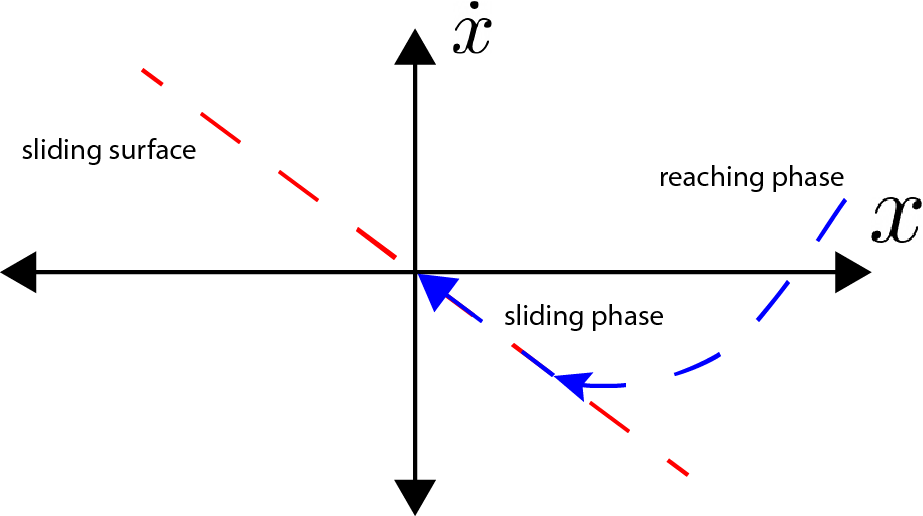
\includegraphics[width=\linewidth]{images/controllers/SMC.png}
    \caption[Illustration of a SMC]{Illustration of a SMC, the two phase of the controller are the reaching phase and the sliding phase. In the reaching phase the sytem drives to the sliding phase. In the sliding phase the controller where the controller attempts to remain on the line by flipping the value of $\sigma$. }
    \label{fig:SMC}
\end{figure}

\subsection{Development of Cooperative Controller and Tuning Methods}

This section will discuss a method of developing a closed-loop assistive controller. First, a simplified system is presented so the controller can be developed. The simplified system consists of two double pendulums connected by a mass-spring dampener at each link. A method of tuning the parameters is presented, along with the effects on effort reduction and system misalignment.

A simplified system was developed to develop the tuning methods. \autoref{fig:double_pend} illustrates the simplified system. Since one set of pendulums is being assisted by the other set, one pendulum is the \textit{assistie} and the other pendulum is the \textit{assisitor} system. The \textit{assisitor} system provides additional torques to help the \textit{assistie} to move through some desired motion. This model and controller are based on the work by Tu \textit{et. al} \cite{tu2020adaptive}, however the system was modified so the \textit{assistie} system is driven by a closed-loop controller. These changes add complexity to the system since the \textit{assistor} system has to handle the errors that arise in the attached closed-loop controller. With two closed-loop systems connected, the controller commands are magnified when handling the errors \cite{tu2020adaptive}. \autoref{fig:controlDiagram} shows the control diagram. The first model has a pendulum that a simple closed-loop PD controller controls. The second model is controlled by an Admittance-Sliding Mode Controller (A-SMC), having useful properties for handling non-linear dynamics and disturbances. Additionally, a gradient descent method auto-tunes the PD controller parameters and the A-SMC. 



\begin{figure}[hbt!]
    \centering
    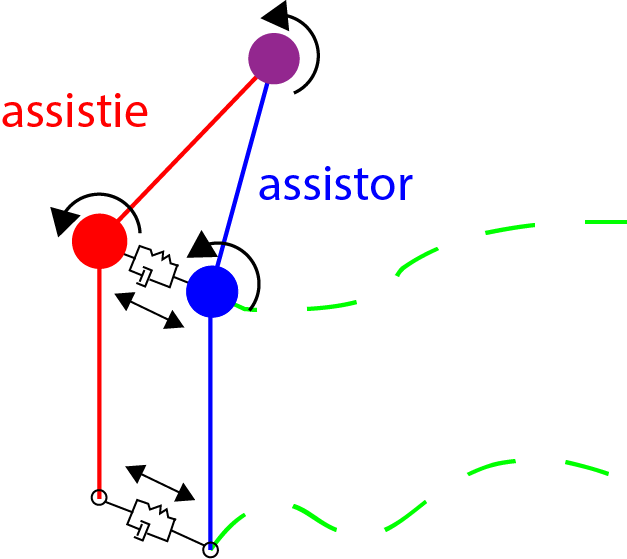
\includegraphics[scale=1.5]{images/controllers/double_pend.png}
    \caption[Double connected pendulum]{Double connected pendulum. Spring-dampeners connect the two pendulum (\textit{assistor} and \textit{assistie}) }
    \label{fig:double_pend}
\end{figure}

\begin{figure}[hbt!]
    \centering
    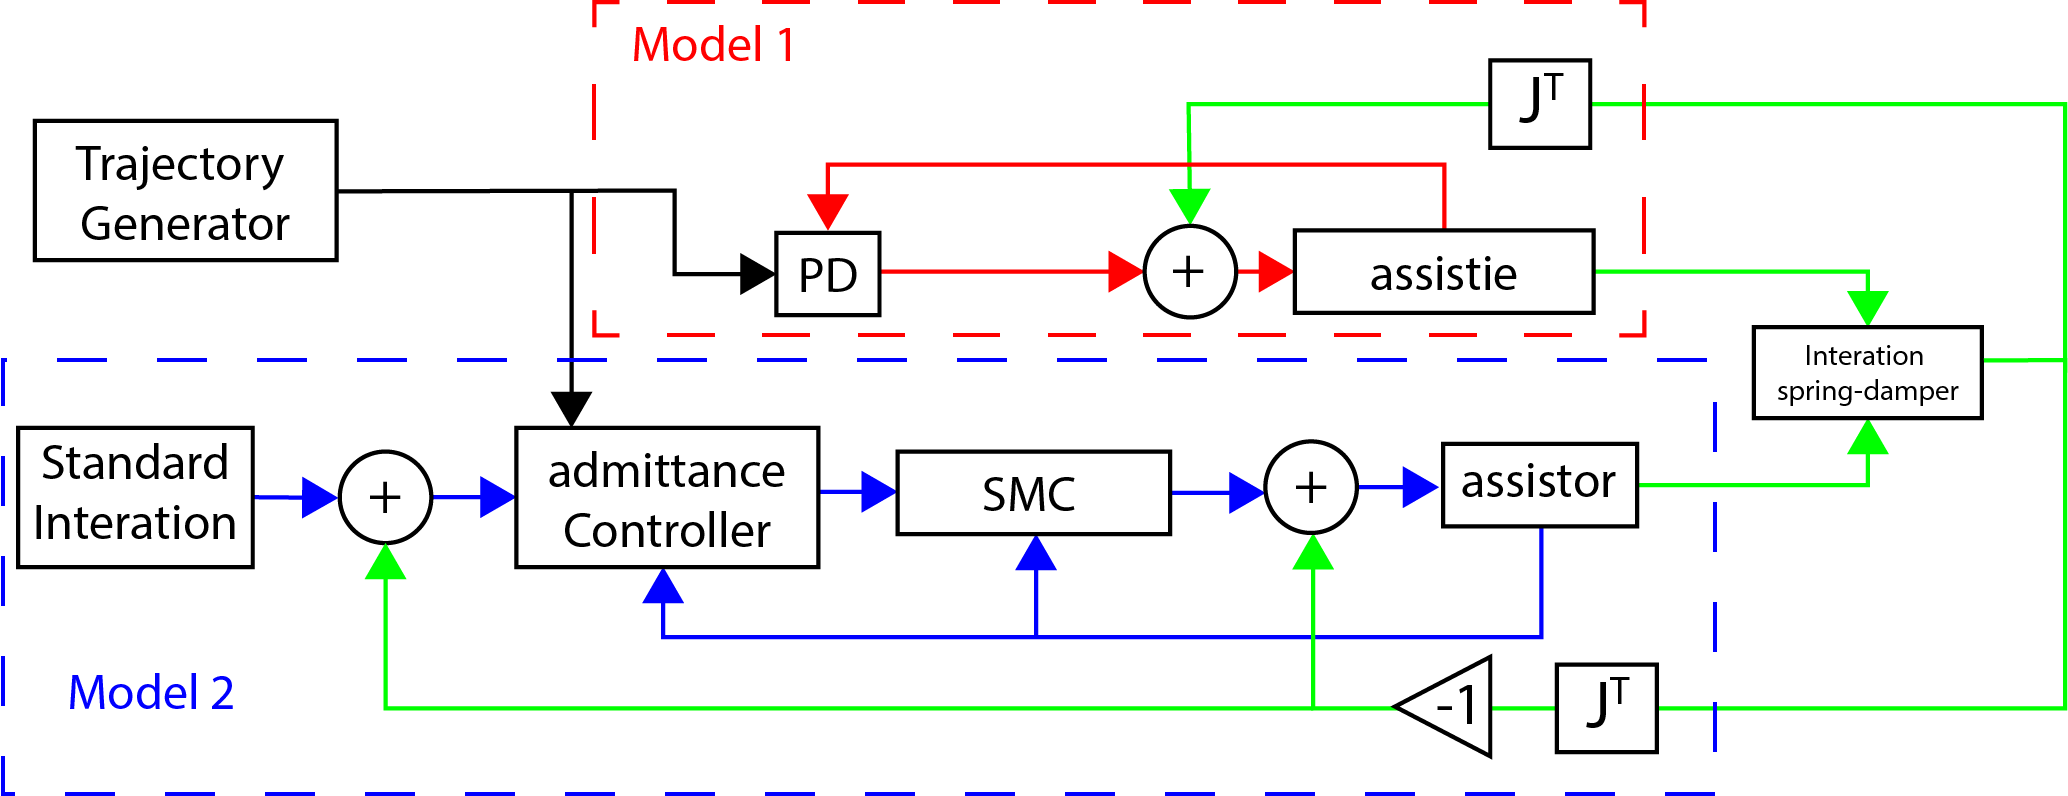
\includegraphics[width=\linewidth]{images/controllers/SMC_control_diagram_overview.png}
    \caption[Control diagram for A-SMC]{Control diagram for A-SMC. Model 1 represents the human model controlled by a simple PD controller and summed with the interaction torques. The Jacobian is used to transform the spring-dampener forces into torques. Model 2 is the exoskeleton controller controlled by the A-SMC. The standard interaction torque is the iLQR controller. The interaction torque is subtracted to lower the applied exoskeleton torque. }
    \label{fig:controlDiagram}
\end{figure}


The problem with A-SMC controllers is the large number of parameters that need to be tuned. These parameters can have non-linear and hard-to-determine effects on the response of the system \cite{slotine1983tracking}. These parameters include SMC parameters and the variable admittance model parameters. Both of which scale with the dimensions of the system. Having a comprehensive method to determine these parameters allows the system to be tuned automatically.  

\autoref{eq:CooPdyn} describes the dynamics for the \textit{assistor} (abbreviated has \textit{tor}) and \textit{assistie} (abbreviated has \textit{tie}) respectively.  It should be noted that $q$ is the joint state for the respective model that they describe. The $F$ terms are the forces generated as a result of being coupled by a spring dampener described by \autoref{eq:coupling}. Additionally, $J$ is the Jacobian of each link to the connection point of the spring dampener system, although any point on the link could be used to calculate the Jacobian matrix, the connection point is at the end of each link. This assumption does not change the process, only the calculation of the Jacobian matrix. It can later be adjusted to the location of the straps of the exoskeleton.

\begin{equation} 
\begin{aligned}
    M_{tor}(q) \ddot{q} + C_{tor} (q,\dot{q}) + G_{tor}(q) &= \tau_{tor} - J_{tor}^T F \\
    M_{tie}(q) \ddot{q} + C_{tie} (q,\dot{q}) + G_{tie}(q) &= \tau_{tie} + J_{tie}^T F
\end{aligned}
    \label{eq:CooPdyn}
\end{equation}

\begin{equation}
    F = K ( \vec{x}_{tor} - \vec{x}_{tie} ) + B (\dot{ \vec{x}}_{tor} - \dot{ \vec{x}}_{tie} ) 
    \label{eq:coupling}
\end{equation}


The \textit{assisitie} system was controlled by \autoref{eq:PDcnrl}; this is a simple PD controller framework. $K_p$ and $K_d$ are gain matrixes and $\vec{q}_d$ is the desired position. This closed-loop controller is intended to be a black-boxed system that could be replaced by an FES or similar systems as discussed above. In this case, we assume that the controller uses the positional feedback from the sensors and fatigue estimation to modulate the applied stimulation. This torque was capped to not exceed an absolute max torque value by using the following method, $ sign(\vec{\tau}_{tie})* min( | \vec{\tau}_{tie}|, \vec{\tau}_{max}) \rightarrow \vec{\tau}_{tie} $ which prevented the controller from generating too high torque. 

\begin{equation}
        \tau_{tie} = K_p( \vec{q}_d - \vec{q}_{tie} ) + K_d ( \dot{\vec{q}}_d - \dot{\vec{q}}_{tie} ) 
    \label{eq:PDcnrl}
\end{equation}

The admittance controls the virtual dynamics of the system and how the systems interact \cite{faulring2005haptic}. If the \textit{assistie} system is capable of following the desired motion, the \textit{assisitor} system will be less aggressive. This interaction is controlled by \autoref{eq:addmittance}, where $x_a$ is the location of the virtual system and $x_d$ is the location of the point on the pendulum link. A separate spring-dampener system is on each of the links of the system. The virtual system is defined by the following terms $M_d$, $B_d$, and $K_d$ are inertia, dampening, and stiffness, respectively. As previously stated, it is desirable to have these parameters adjust on the fly to the intention and ability of the \textit{assistie} system. The variability is controlled by \autoref{eq:intention} and \autoref{eq:varible}. Here $\gamma_{n,p}$ and $\alpha_{n,p}$ are tuning variables for the damping and stiffness of the admittance controller. The admittance will control how quickly and aggressively the \textit{assistor} system will respond. If the stiffness or dampening is too large, the model will not track the desired motion.   

\begin{equation}
    \begin{aligned}
        \tau_{int} &= M_d^{-1}( K_d e_a + B_d \dot{e}_a)  \\
        e_a &= x_a - x_d 
    \end{aligned}
    \label{eq:addmittance}
\end{equation}

\begin{equation}
    \begin{aligned}
         intent &= bool ( sign(T_h) == sign(\dot{q}_d) ) \\
         \mu &= \Big|\frac{T_h}{T_{id}} \Big|
    \end{aligned}
    \label{eq:intention}
\end{equation}



\begin{equation}
    \begin{bmatrix} K_d \\ B_d \end{bmatrix} = \begin{cases}
        \begin{bmatrix} K_{p} \\ B_{p} \end{bmatrix} + \mu  \begin{bmatrix} \alpha_p  \\ \gamma_p \end{bmatrix}, intent = 1 \\
        \begin{bmatrix} K_{n} \\ B_{n} \end{bmatrix} - \mu  \begin{bmatrix} \alpha_n  \\ \gamma_n \end{bmatrix}, intent = 0
  \end{cases}
  \label{eq:varible}
\end{equation}


The A-SMC controller suffers from an abundance of tunable parameters. The admittance controller and SMC have parameters requiring synergistic tuning since these systems are connected. A gradient descent method is used to find optimal parameters based on various cost functions and constraints for the controller. Gradient descent is used since it should arrive quickly to a solution  \cite{piltan2012performance} \cite{wang1996course}. The goal is to minimize the objective function by updating parameters. This method will iterate until the objective function converges to a locally optimal location. The tunable parameters for this controller are the variable admittance parameters ($K_{n,p}$, $B_{n,p}$, $\alpha_{n,p}$, $\gamma_{n,p}$) and the sliding mode controller variables ($\rho$, $\Lambda$, $\beta$).  Another important variable is the limit of the torque that the \textit{assistor} system can provide, and this limitation is important since real physical systems cannot produce infinite torque. Motors and gearboxes present real limitations on the system. This method allows for the maximum torque to be used, has a hard limitation, and allows for the minimal limit to be found.


The optimization was calculated using Simulink Response Optimization\footnote{https://www.mathworks.com/help/sldo/response-optimization.html}. Several cost functions were tested to find the optimal performance, and the model was trained to follow a polynomial trajectory. Root mean squared error (RMSE) was used for the cost function shown in \autoref{eq:RMSE} of the \textit{assistor} system, where $x$ is the observation and $\hat{x}$ is the reference, either position or velocity. The error is summed along both the trajectory and the joints to get a scalar value. If both the position and velocity RMSE are used, they are summed.

The gain parameters $K_p$ and $K_d$ in \autoref{eq:PDcnrl} were also tuned using the same method. The controller assumed that no assistance was provided by the \textit{assistor} system. These gains were set for the \textit{assistie} controller in the closed-loop system.

\begin{equation}
    e = \sqrt{ \frac{ \sum_i=1^N ( \hat{x}_i - x_i )^2 }{N}  }
    \label{eq:RMSE}
\end{equation}

\subsubsection{Tuning of Cooperative Controller}
Several different cost functions were tested to arrive at a cost function for parameter tuning. It was assumed that the \textit{assistie} system. Three different cost functions were tested, one based on position, another on velocity, and finally, one used both position and velocity.


\autoref{fig:cost_function_optimization} shows the conversions of the cost functions used for optimization. All the cost functions converged to a steady value after approximately ten iterations; this means that the tuned controllers' parameters reached a local point where the system's performance was steady as defined by the cost. The convergence of the cost function is not a direct correlation to the actual system performance. By examining the system's state space, the performance of the controller can be better determined.





\begin{figure}[ht]
    \begin{subfigure}{0.5\textwidth}
        \centering
        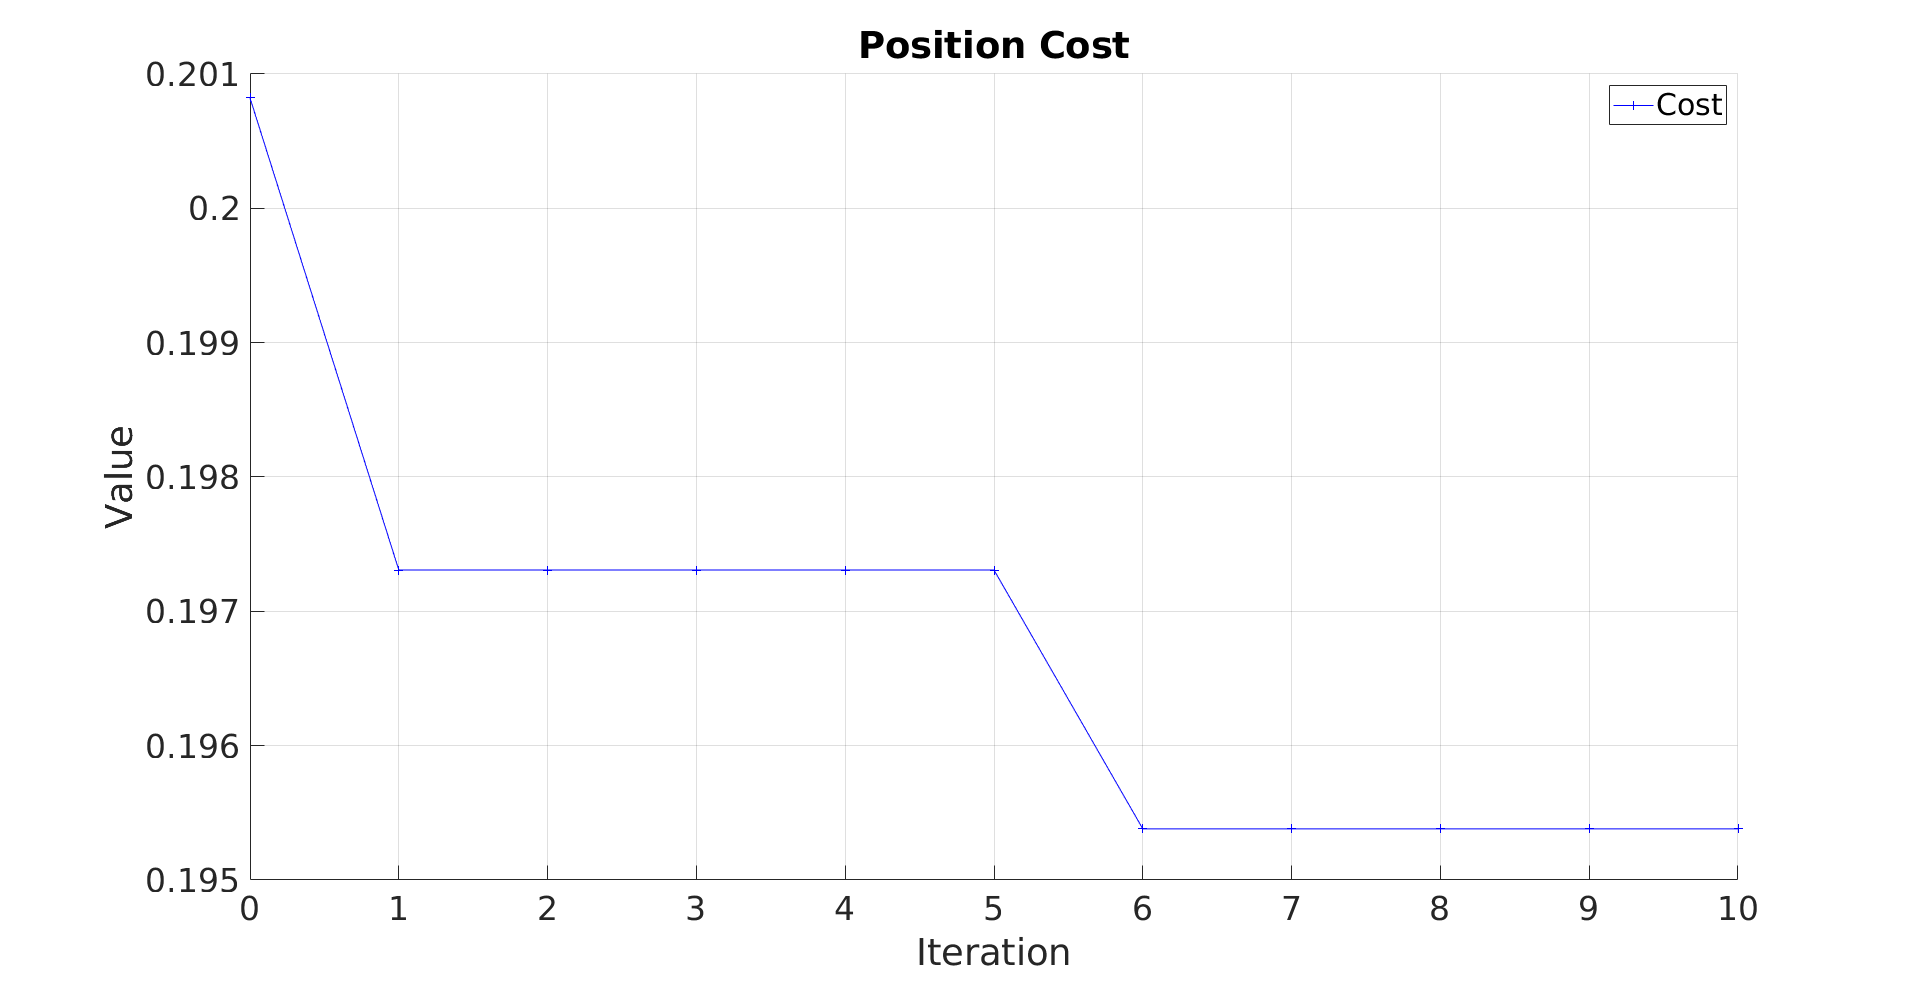
\includegraphics[width=0.9\linewidth]{images/controllers/pos_cost.png}
        \caption[Position cost function]{Convergence of position cost function}
        \label{fig:pos_cost}
    \end{subfigure}
    \begin{subfigure}{0.5\textwidth}
        \centering
        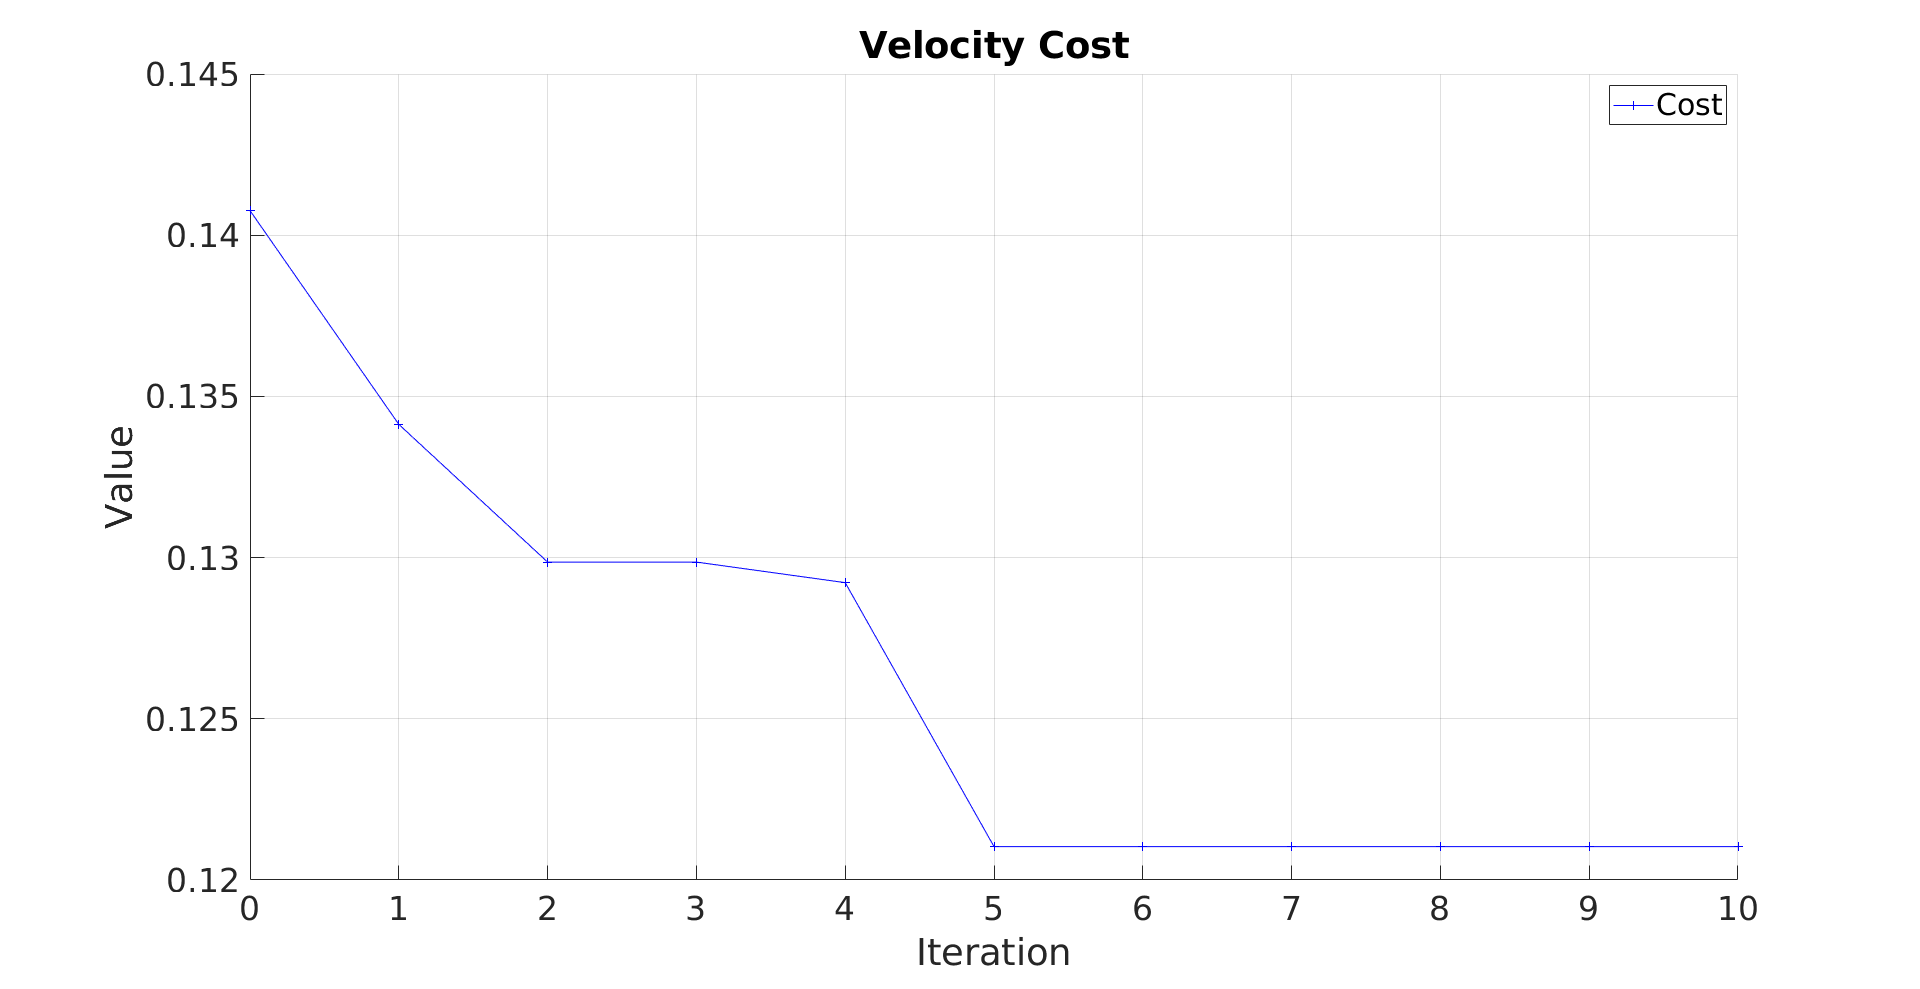
\includegraphics[width=0.9\linewidth]{images/controllers/vel_cost.png}
        \caption[Velocity cost function]{Convergence of velocity cost function}
        \label{fig:vel_cost}
    \end{subfigure}

    \begin{subfigure}{\textwidth}
        \centering
        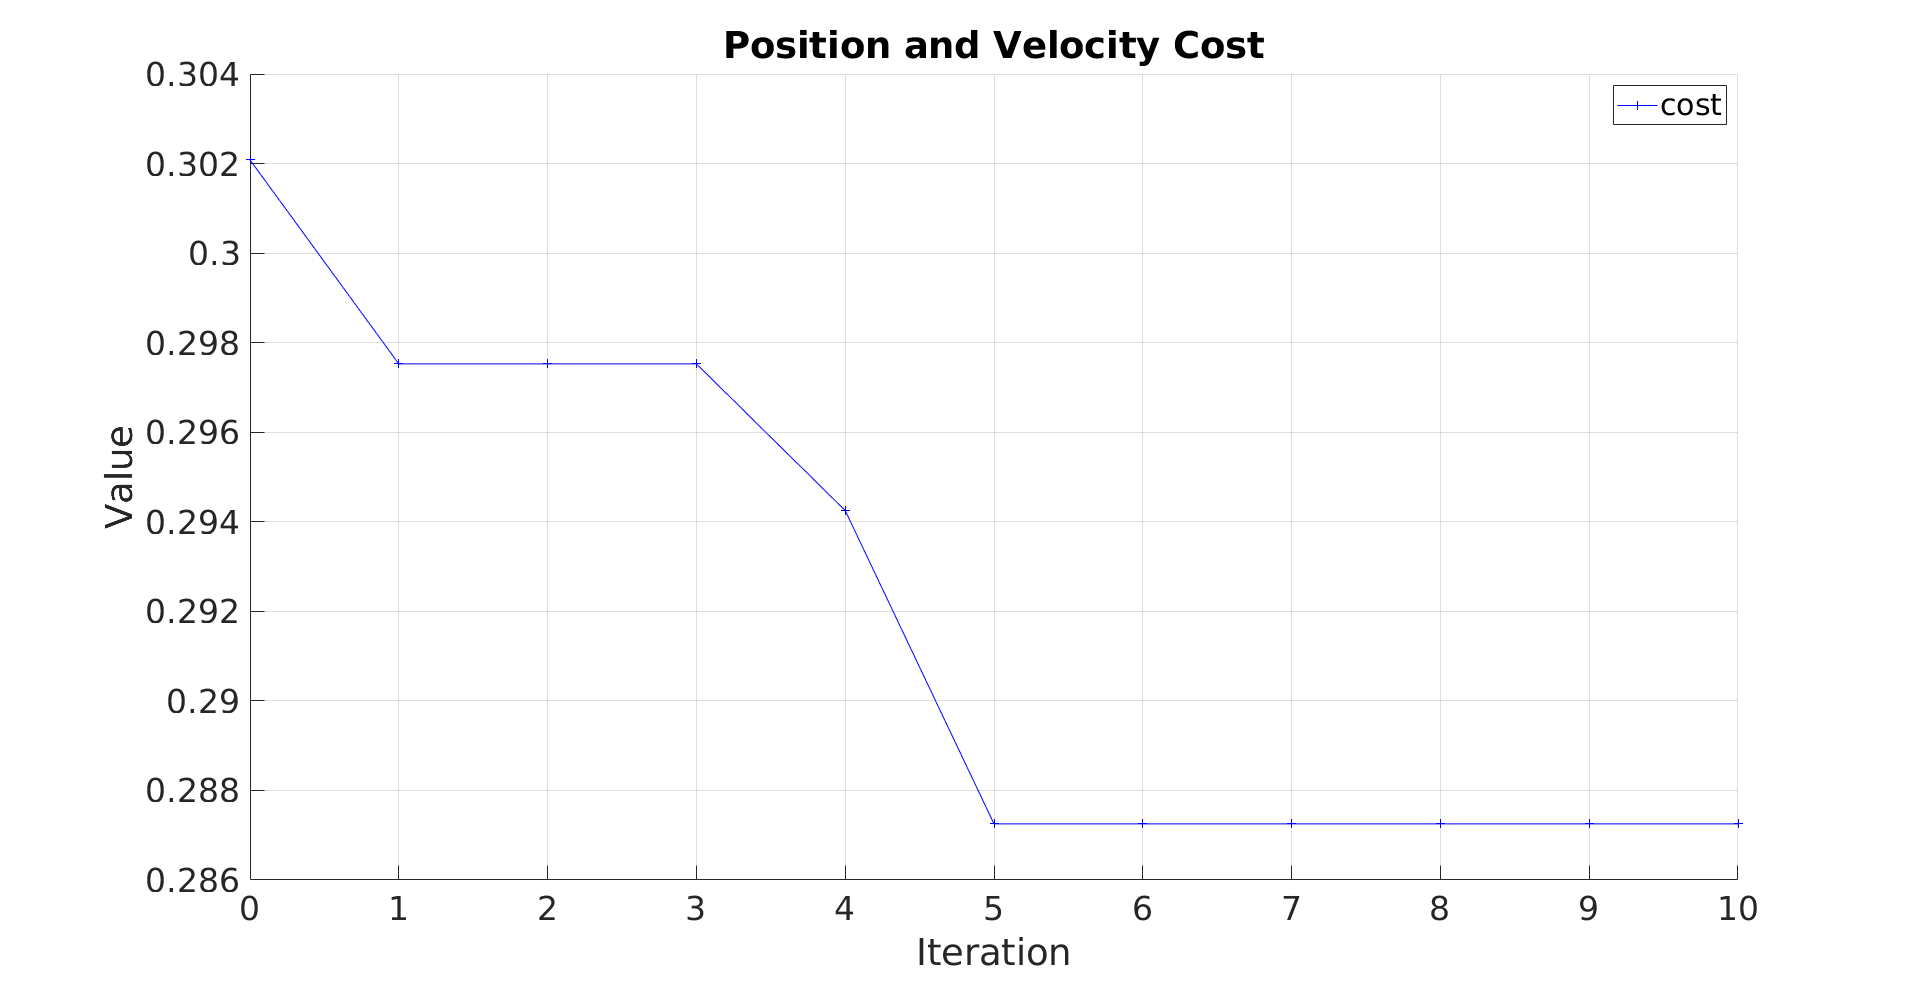
\includegraphics[width=0.45\linewidth]{images/controllers/all_cost.png}
        \caption[Combined cost function]{Convergence of combined cost function}
        \label{fig:all_cost}
    \end{subfigure}
    \caption[Convergence for Different Cost Functions]{Convergence for Different Cost Functions}
    \label{fig:cost_function_optimization}
\end{figure}


The state-space of the system response is shown in  \autoref{fig:statespace}. The output of each of the tuning methods was compared throughout this paper. The untuned gains are also shown for reference to show the improvement of the output. The response optimizer was tuned until the cost function converged. The untuned gains performed poorly and were able to reach the settling point. Using the position tuning caused a significant spike in the sliding surface for both joints. Using position and velocity had similar results as just using velocity to the cost function. 


\begin{figure}[ht!]
    \centering
    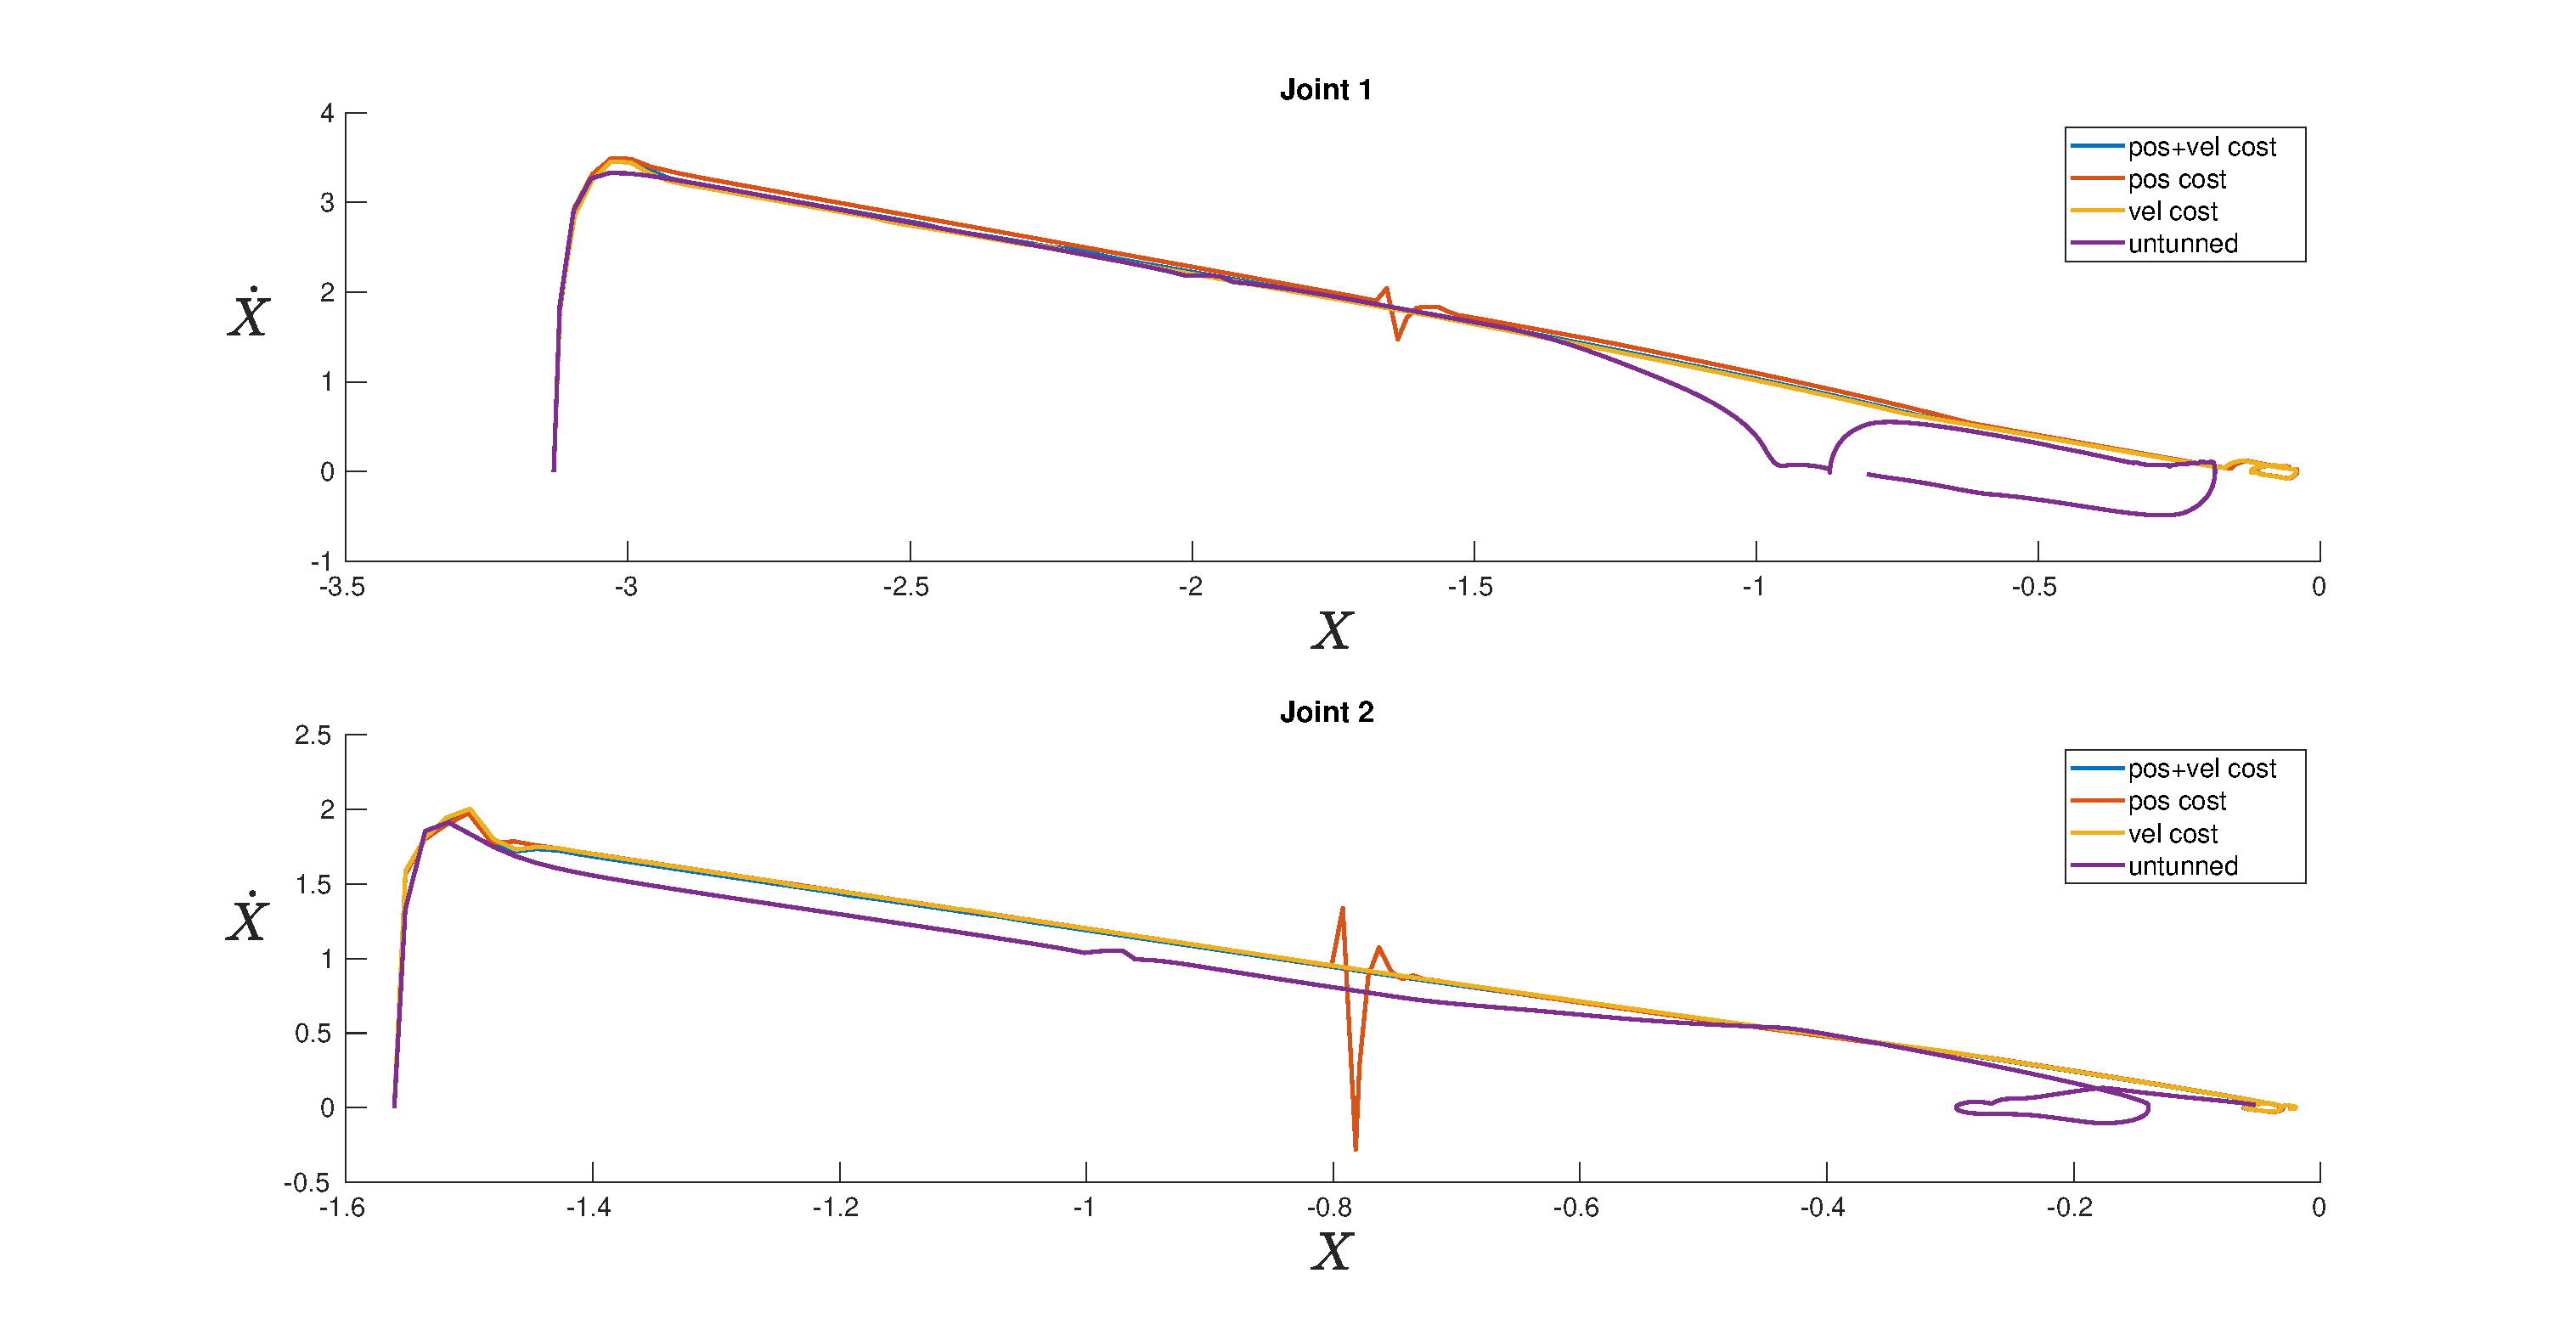
\includegraphics[width=\linewidth]{images/controllers/statespace.eps}
    \caption[A-SMC State Space]{Comparing different cost functions used to tune the A-SMC controller}
    \label{fig:statespace}
\end{figure}

Different involvement of the \textit{assistie}  using the tuned gains, reduced involvement, time-varying, and no involvement were tested. Additional varying alignment methods were tested to show the effect of the systems not being perfectly aligned with the length of the \textit{assistor}; this is important since the joints of the exoskeleton may not be perfectly aligned with the joint of the human. Misalignment can be caused by the exoskeleton not being put on properly or slipping while in motion. This misalignment causes different forces to act on the system that the controller. The controller needs to be able to compensate for these forces and still track the desired motion. The alignment methods included changing the links by $\pm 5\%$ of the \textit{assistie} link lengths. This misalignment simulates the exoskeleton joints being too high and too low along the length of the human leg. \autoref{fig:no_effort} shows the effects with no involvement from the \textit{assistie} system. All the effort is being supplied by the \textit{assistor} system's A-SMC. As shown \autoref{fig:no_effort_traj}, the controller was able to track the desired trajectory. 

\begin{figure*}[h!]
    \centering
    \begin{subfigure}{0.5\textwidth}
        \centering
        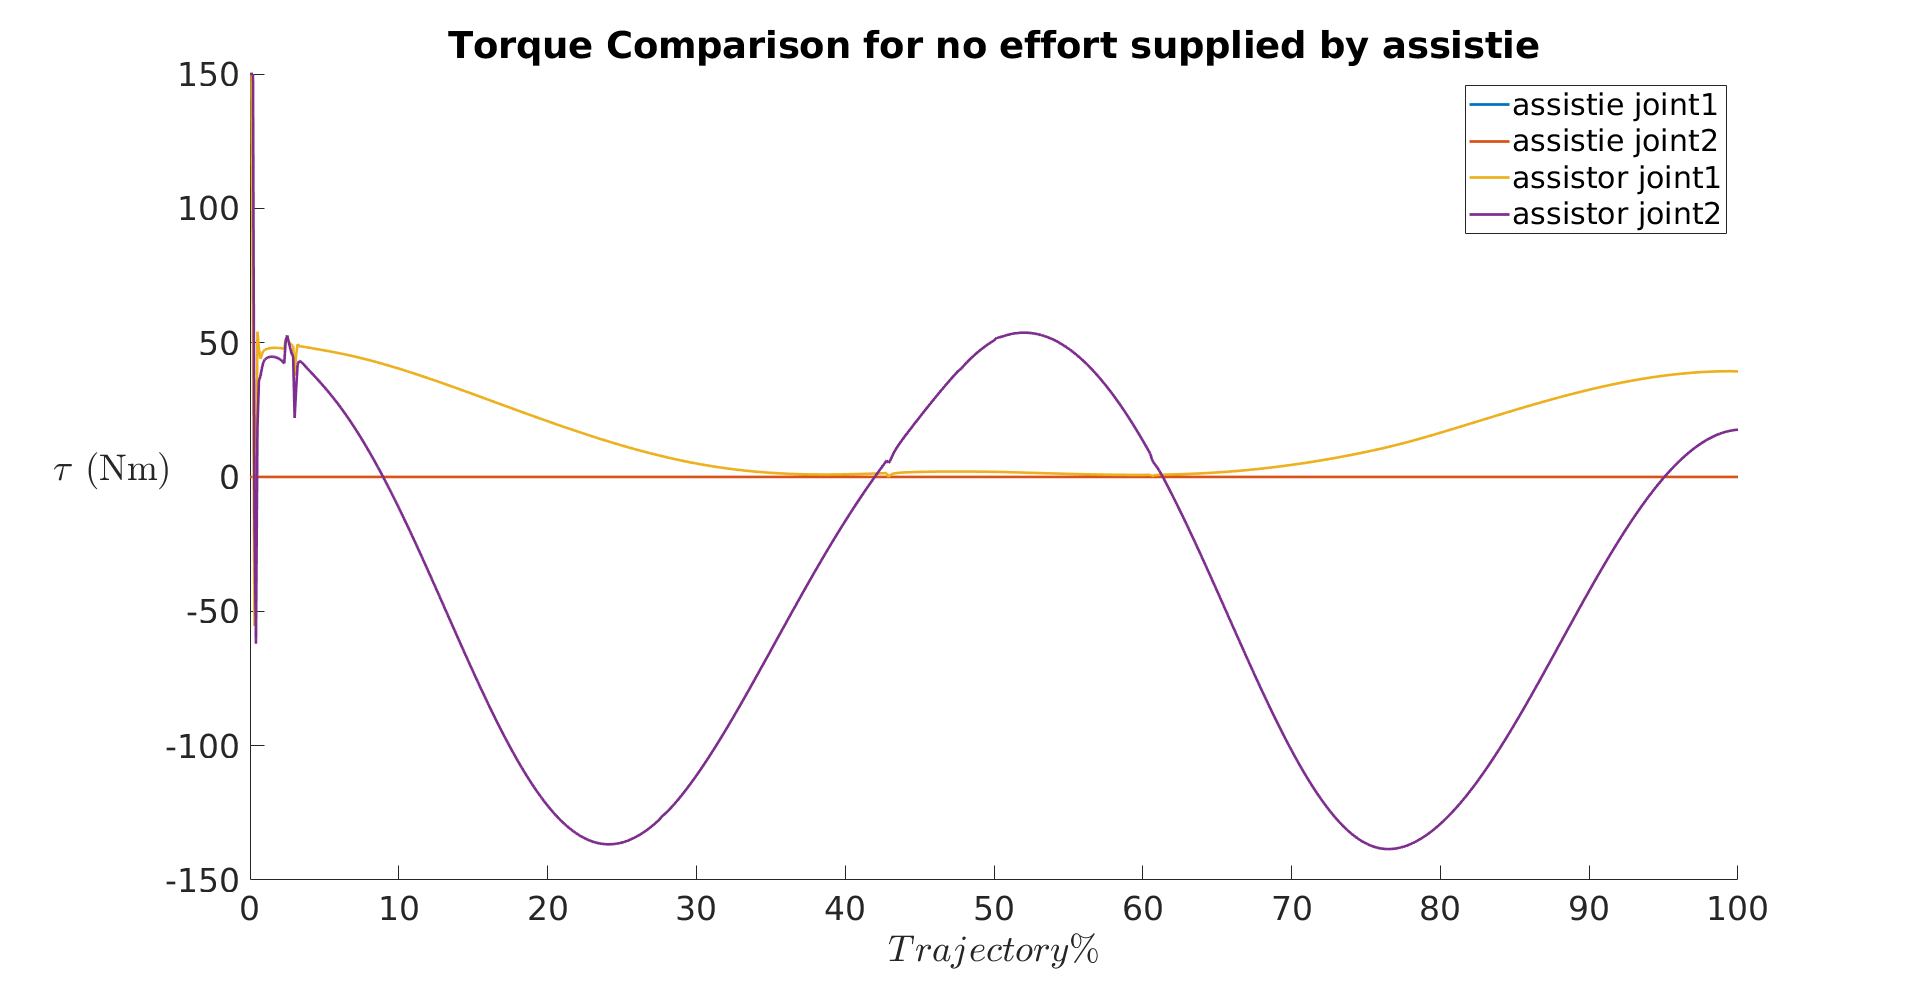
\includegraphics[width=\linewidth]{images/controllers/none_torque.png}
        \caption[Double Pendulum: No Torque-Effort]{Torque applied to the double pendulum}
        \label{fig:no_effort_torque}
    \end{subfigure}%
    ~
    \begin{subfigure}{0.5\textwidth}
        \centering
        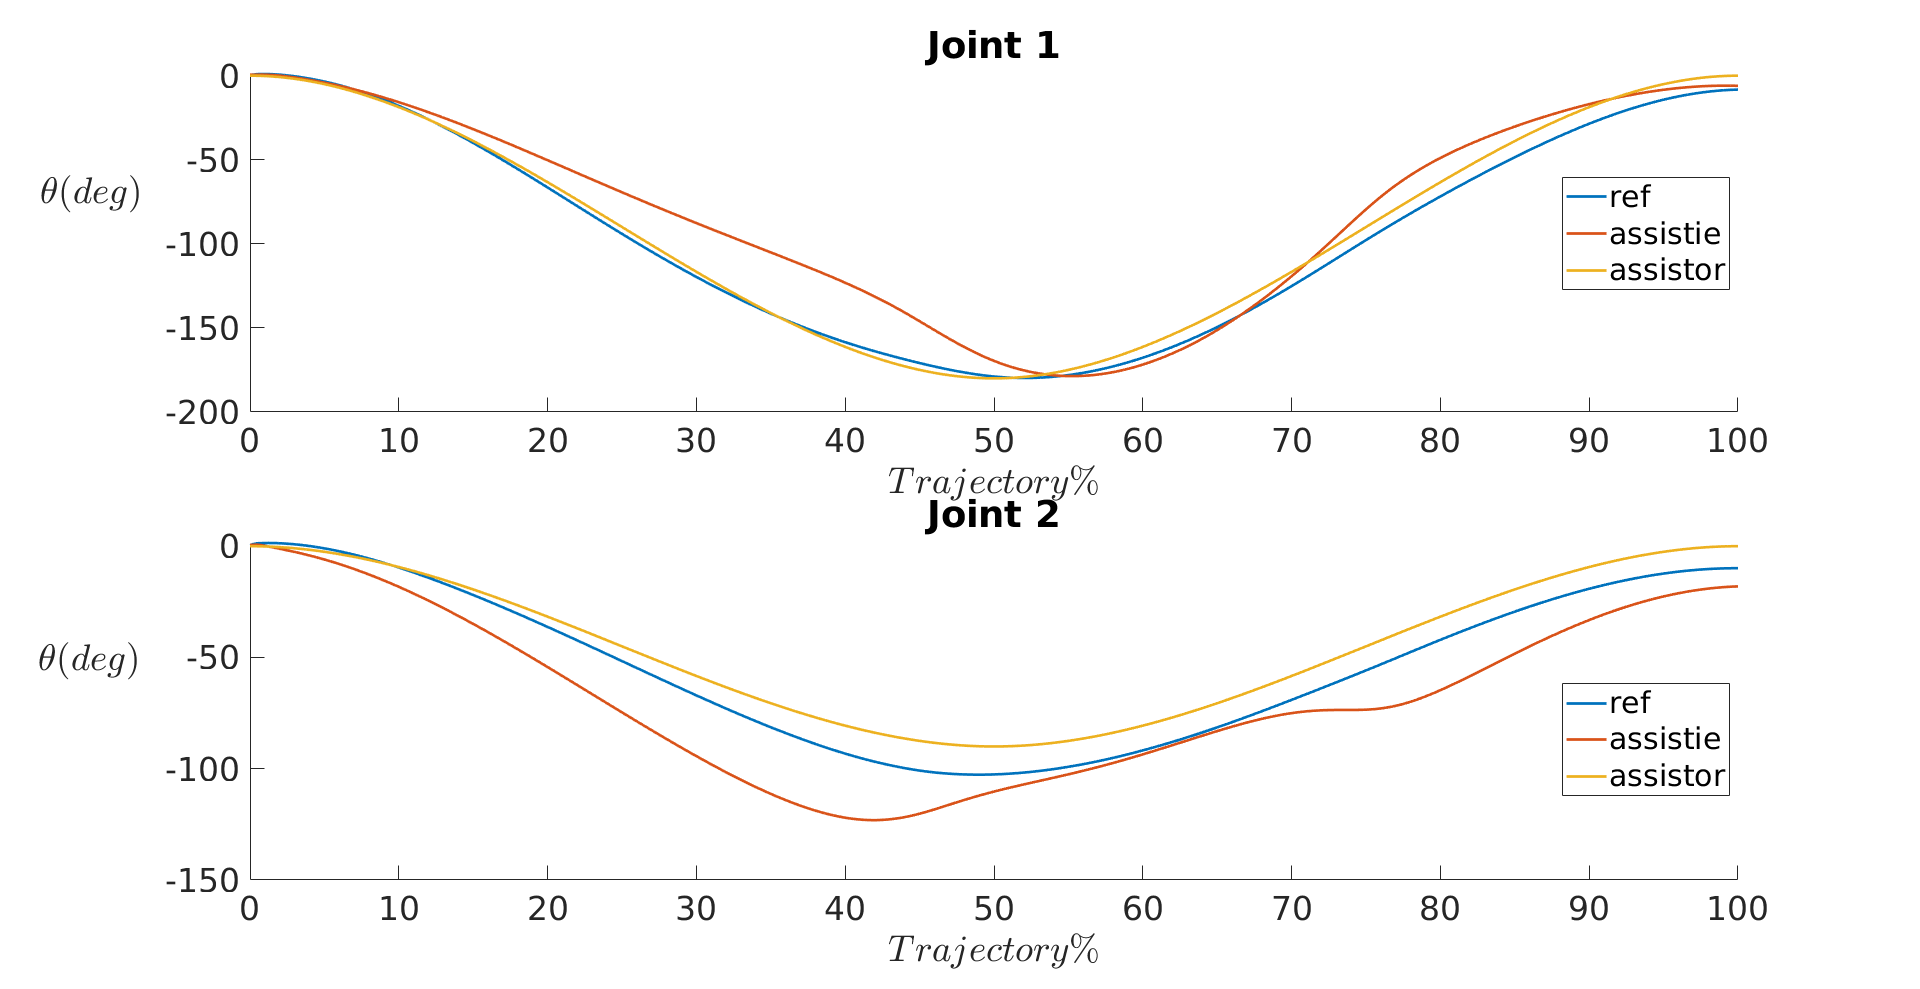
\includegraphics[width=\linewidth]{images/controllers/none_traj.png}
        \caption[Double Pendulum: No Torque-Trajectory]{Trajectories of double pendulum}
        \label{fig:no_effort_traj}
    \end{subfigure}
    \caption[Double Pendulum: No Torque]{Double pendulum model responses with no \textit{assistie} torques.}
    \label{fig:no_effort}
\end{figure*}

\autoref{fig:reduced_effort} shows the effects with a reduced involvement from the \textit{assistie} system. The \textit{assistie} system was only capable of producing approximately 20\%  of the required torque. The PD controller controlling the \textit{assistie} system worked together with the A-SMC controlling the \textit{assistor} to track the desired motions. The controller was not re-tuned for the \textit{assistor} interaction. The same gains found during no \textit{assistor} interaction were used. 

\begin{figure*}[h!]
    \centering
    \begin{subfigure}{0.5\textwidth}
        \centering
        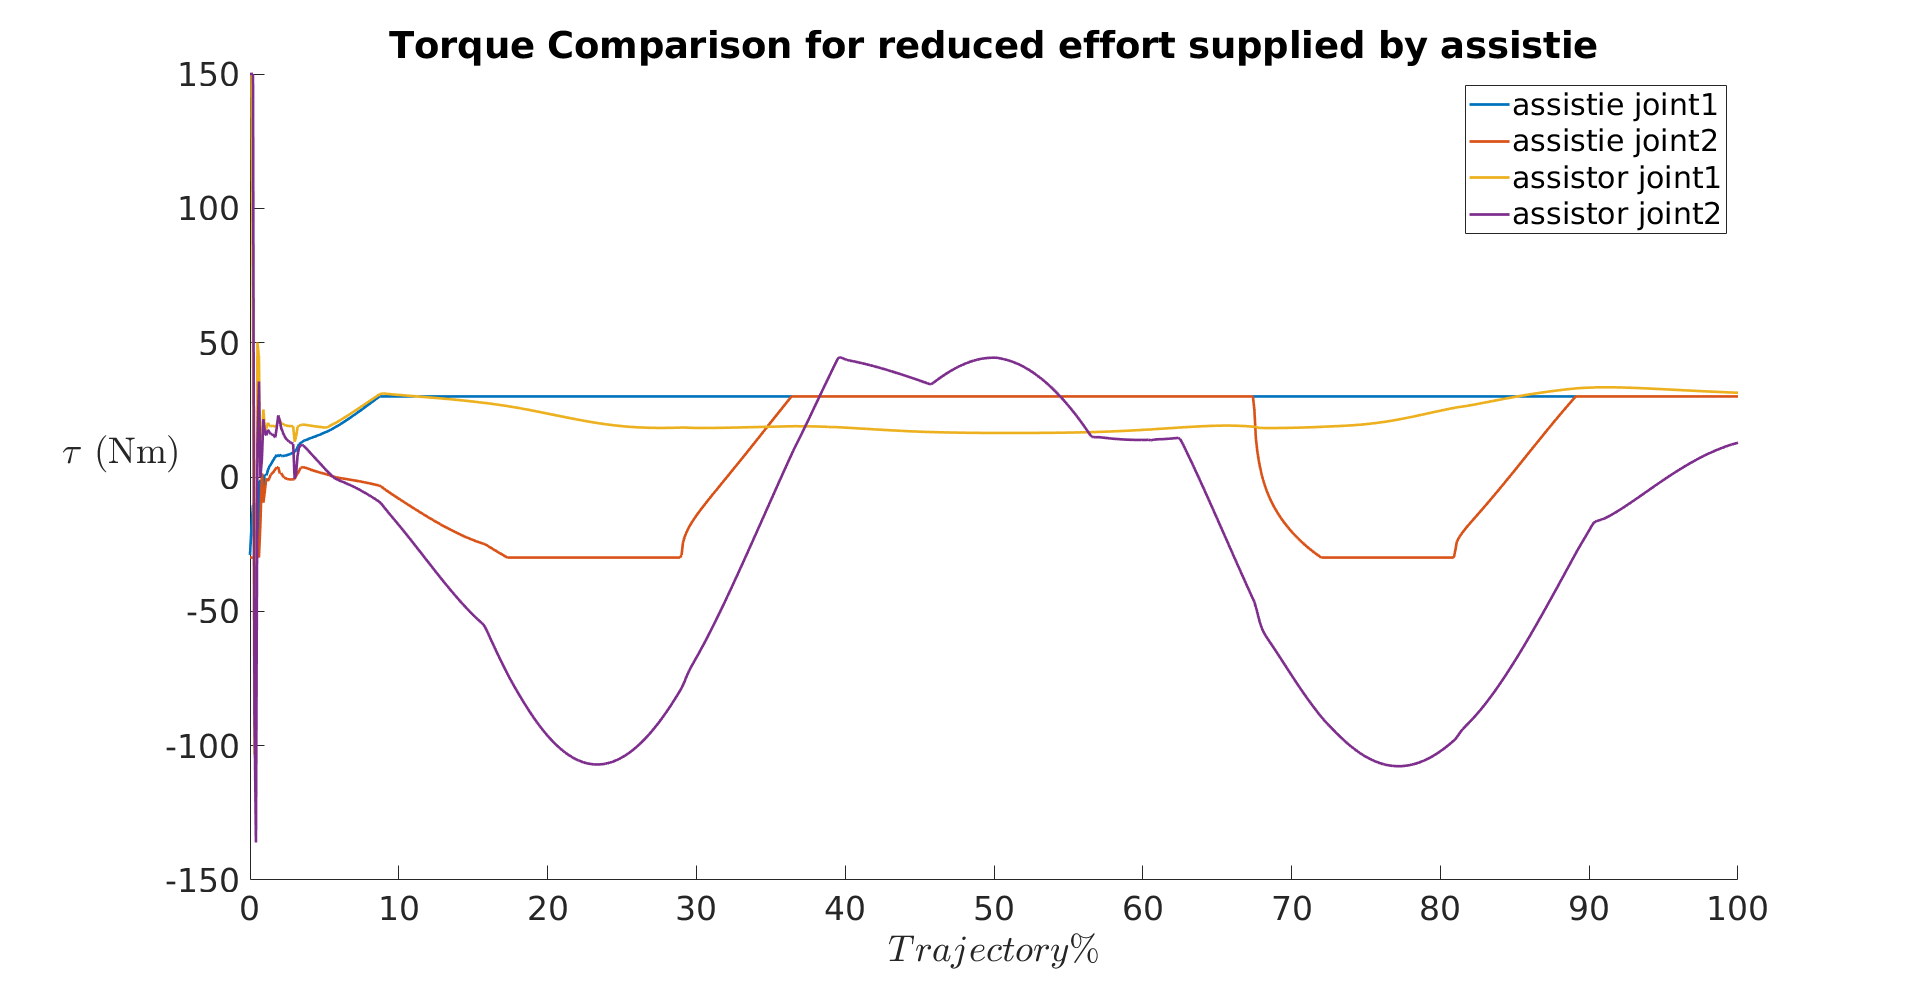
\includegraphics[width=\linewidth]{images/controllers/reduced_torque.png}
        \caption[Double Pendulum: Reduced Torque-Effort]{Torque applied to the double pendulum}
        \label{fig:reduced_effort_torque}
    \end{subfigure}%
    ~
    \begin{subfigure}{0.5\textwidth}
        \centering
        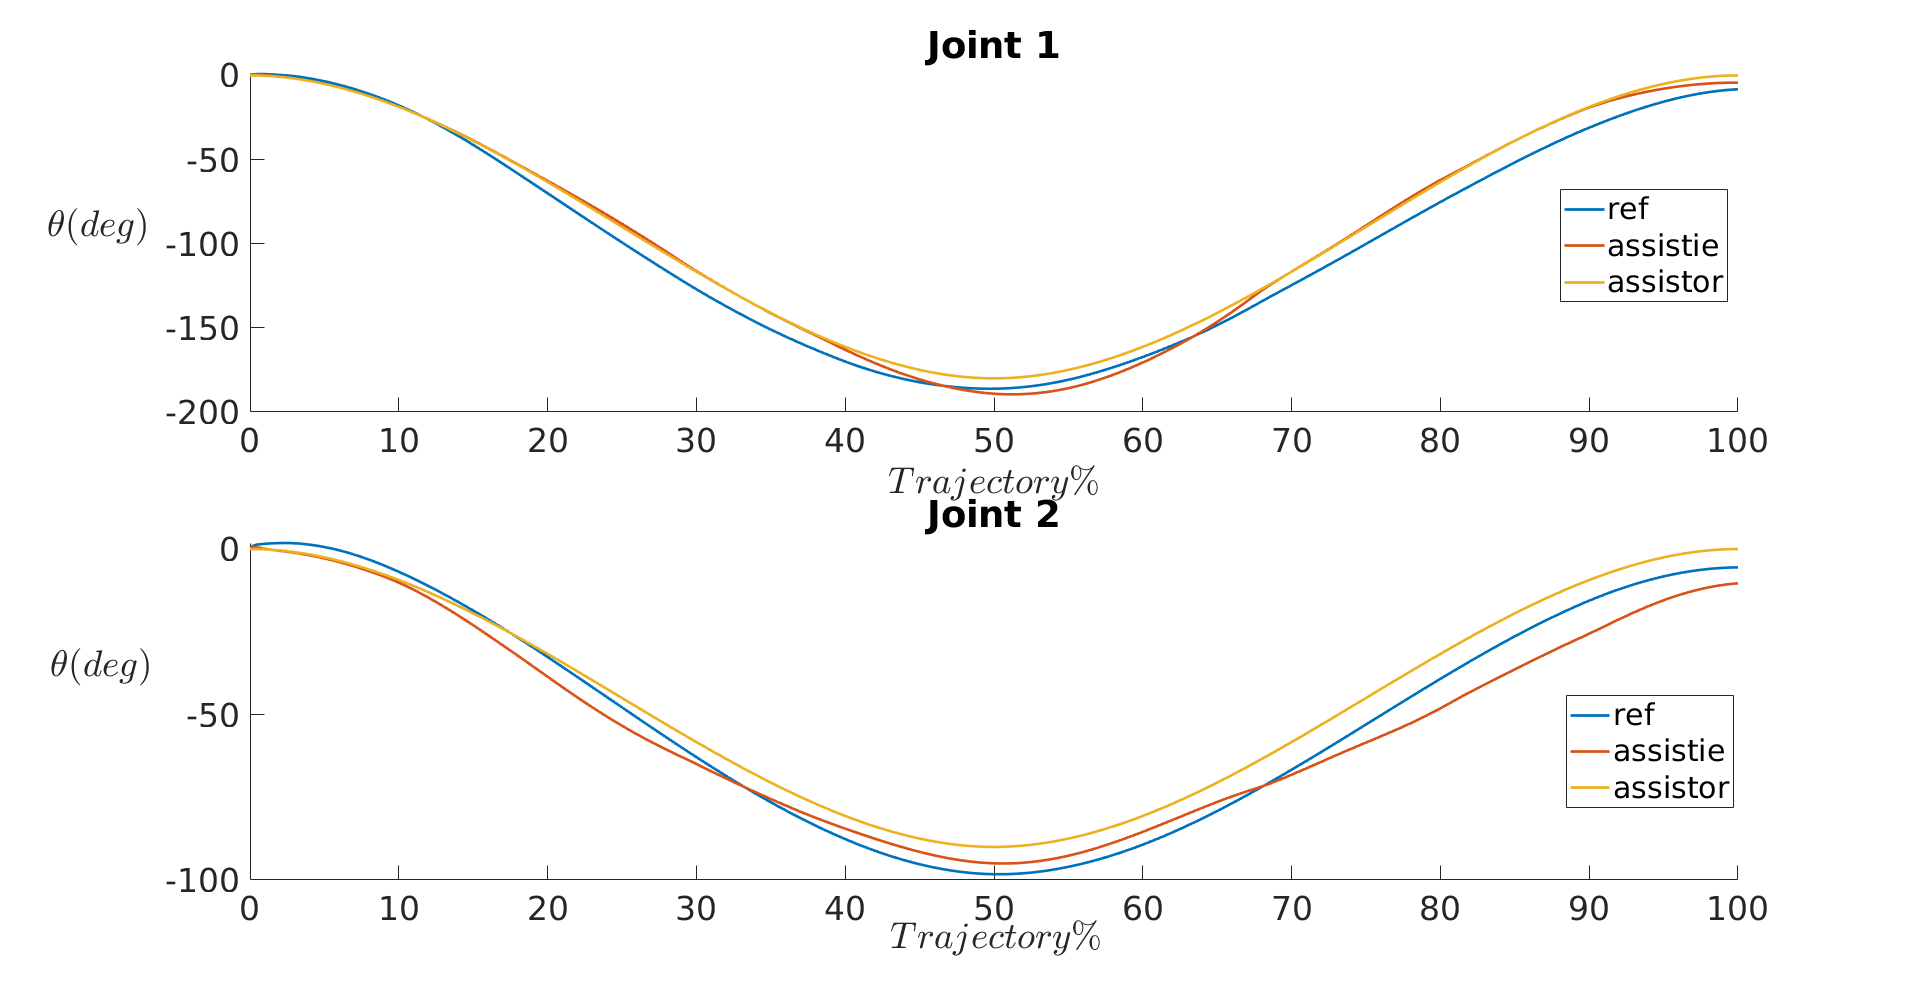
\includegraphics[width=\linewidth]{images/controllers/reduced_traj.png}
        \caption[Double Pendulum: Reduced Torque-Trajectory]{Trajectories of double pendulum}
        \label{fig:reduced_effort_traj}
    \end{subfigure}
    \caption[Double Pendulum: Reduced Torque]{Double pendulum model responses with reduced \textit{assistie} torques.}
    \label{fig:reduced_effort}
\end{figure*}

\autoref{fig:time_varying} shows the effects with a reduced involvement from the \textit{assistie} system. The \textit{assistie} system was only capable of producing approximately 20\%, and it was reduced over time by multiplying it $e^{-\xi t}sin(t)$; this was done to simulate a reduction in torque over time. The A-SMC controlling the \textit{assistor} had to handle the change in involvement over time. 

\begin{figure}[h]
    \centering
    \begin{subfigure}{0.5\textwidth}
        \centering
        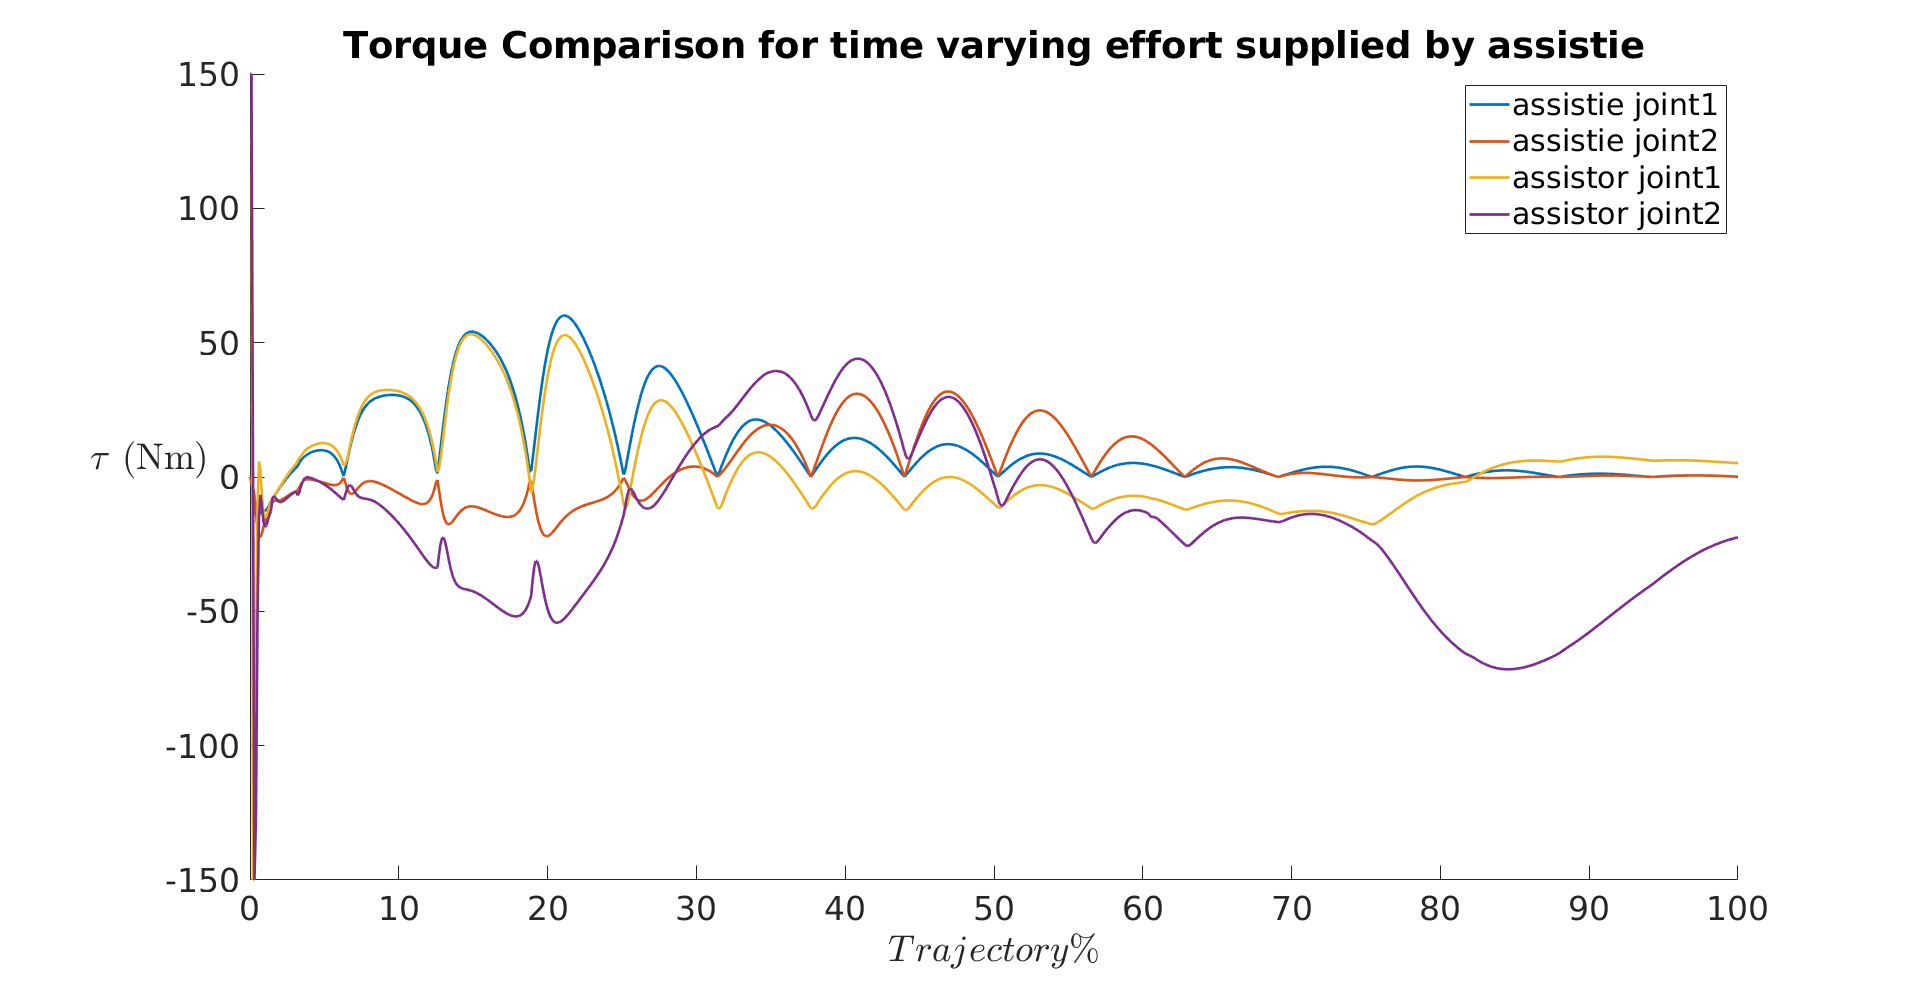
\includegraphics[width=\linewidth]{images/controllers/time_varying_torque.png}
        \caption[Double Pendulum: Time varying Torque-Effort]{Torque applied to the double pendulum}
        \label{fig:time_varying_torque}
    \end{subfigure}%
    ~
    \begin{subfigure}{0.5\textwidth}
        \centering
        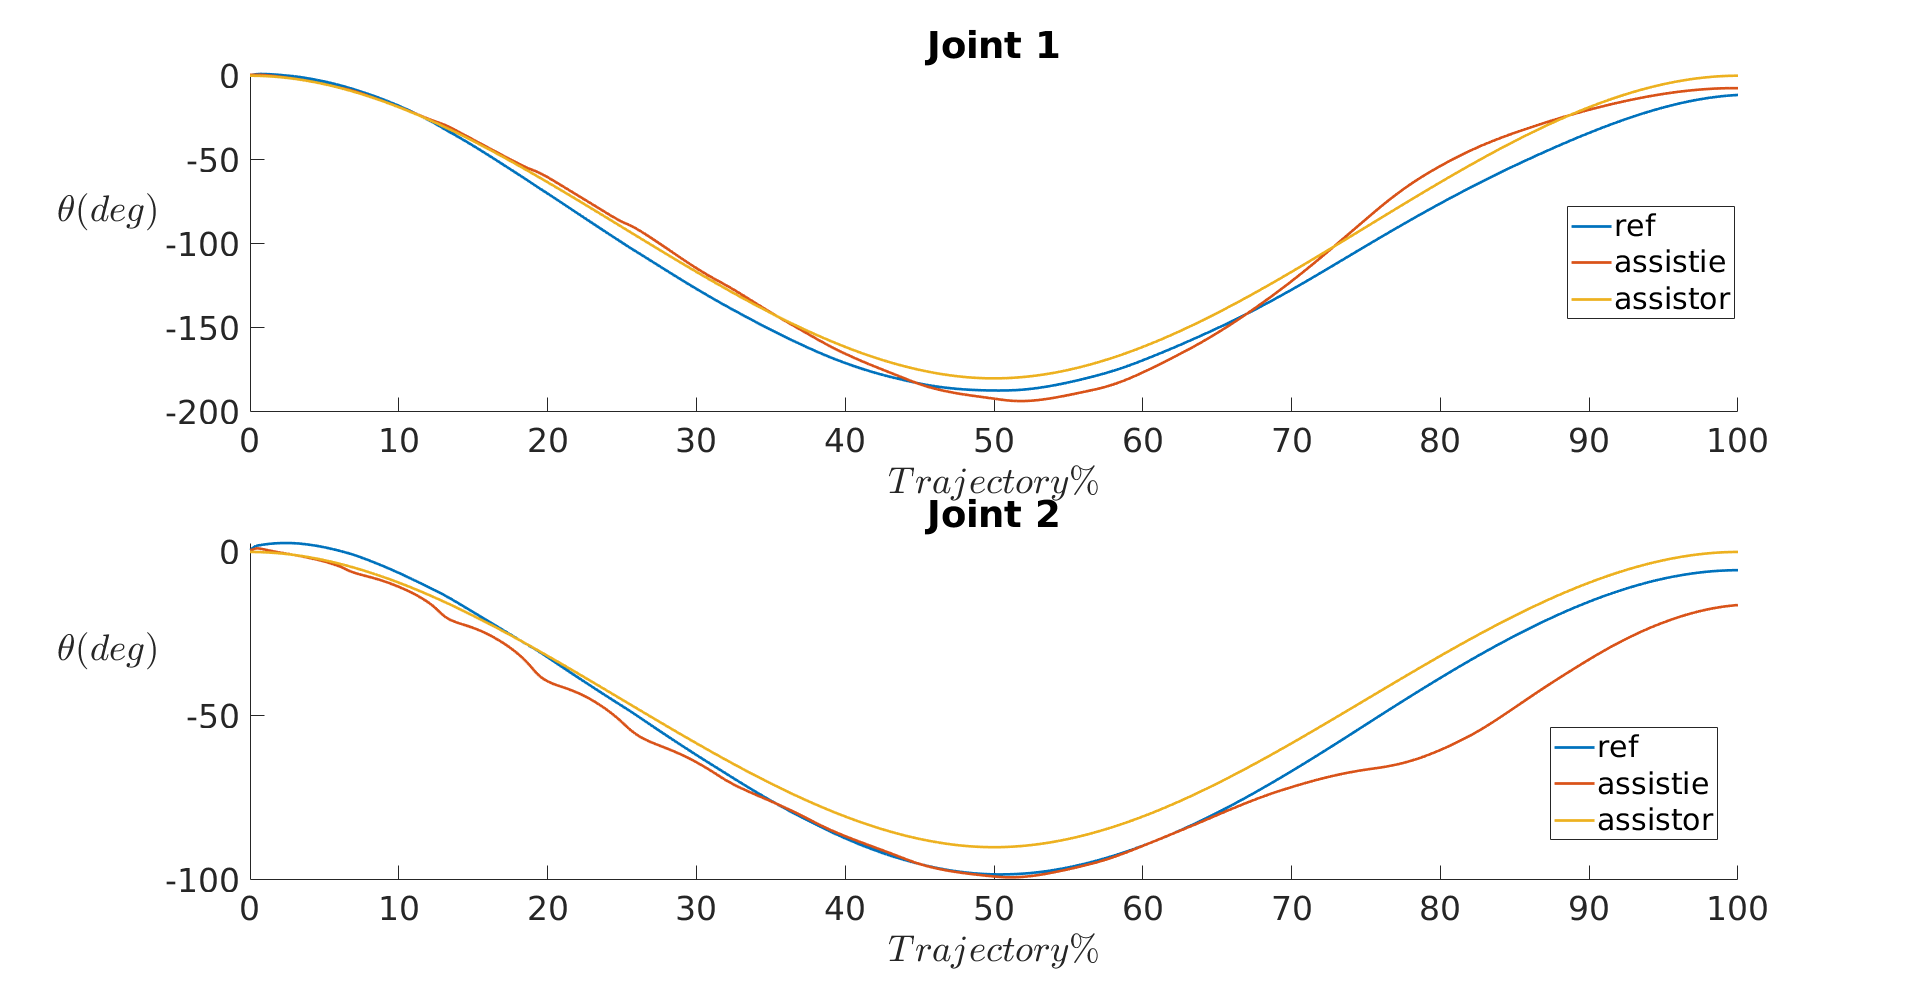
\includegraphics[width=\linewidth]{images/controllers/time_varying_traj.png}
        \caption[Double Pendulum: Time Varying Effort-Trajectory]{Trajectories of double pendulum}
        \label{fig:time_varying_traj}
    \end{subfigure}
    \caption[Double Pendulum: Time Varying Torque]{Double pendulum model responses with time varying reduced \textit{ assistie} torques.}
    \label{fig:time_varying}
\end{figure}


Additionally, the effects of the controller were tested with a misalignment between the \textit{assistie} and \textit{assistor} systems. The time-varying control signal was used for these tests. The length of the \textit{assistor} system was changed by $\pm 5\%$; this would simulate an exoskeleton that does not perfectly align with the person. \autoref{fig:misalignmentIllistration} shows the misalignment between  the \textit{assistor} and \textit{assistie} systems. The dotted circles show the offset locations of the connection points. This misalignment also changes the direction of the interaction forces and will pull the \textit{assistie} system in different directions. The effects are shown in misalignment are shown in \autoref{fig:small_length} and \autoref{fig:larger_length}.


\begin{figure}
    \centering
    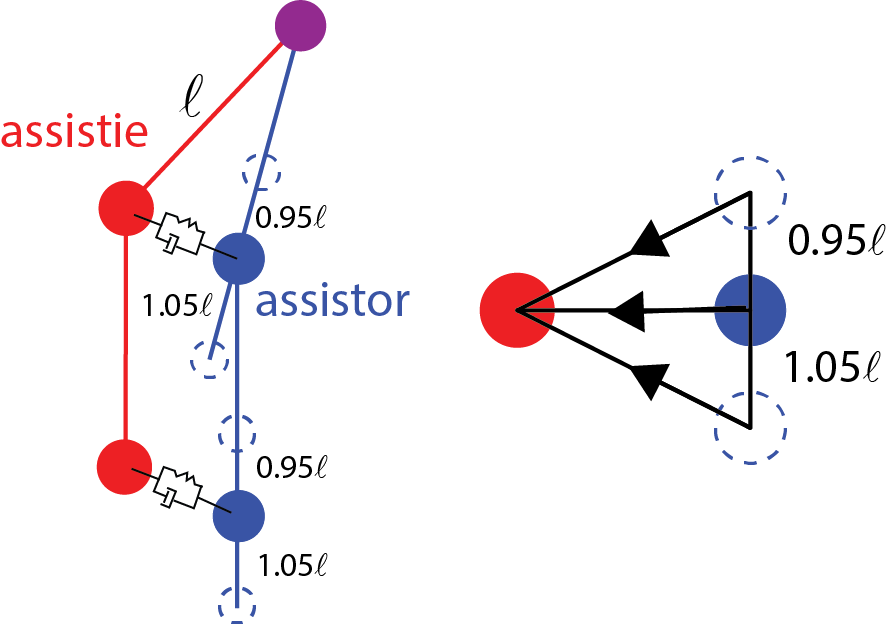
\includegraphics{images/controllers/alignment_comparison.png}
    \caption[Illustration of the pendulum misalignment of ]{Illustration of misalignment between the  \textit{assistor} and  \textit{assistie} systems. The dotted circles represents the misalignment location of the system. This also changes the location of the spring-dampener connection point.  }
    \label{fig:misalignmentIllistration}
\end{figure}

\begin{figure}[h!]
    \centering
    \begin{subfigure}{0.5\textwidth}
        \centering
        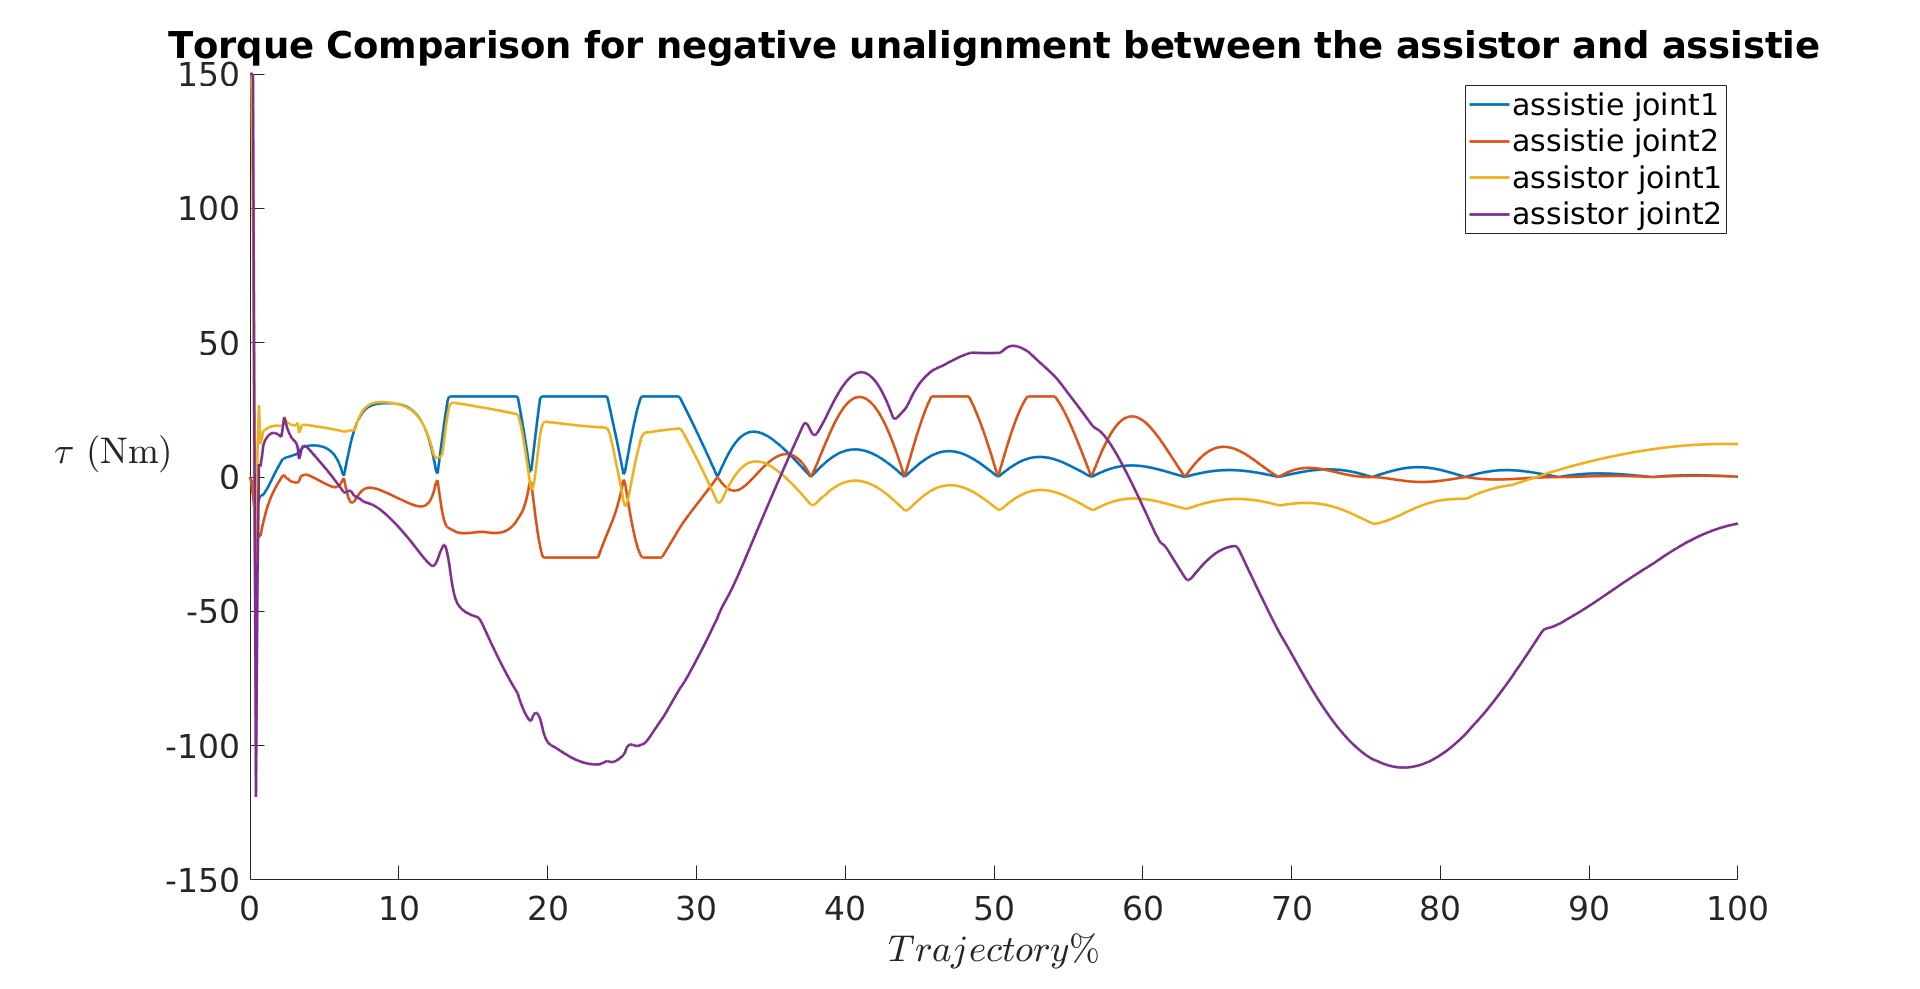
\includegraphics[width=\linewidth]{images/controllers/small_length_torque.png}
        \caption[Double Pendulum: Negative Alignment-Effort]{Torque applied to the double pendulum}
        \label{fig:small_length_torque}
    \end{subfigure}%
    ~
    \begin{subfigure}{0.5\textwidth}
        \centering
        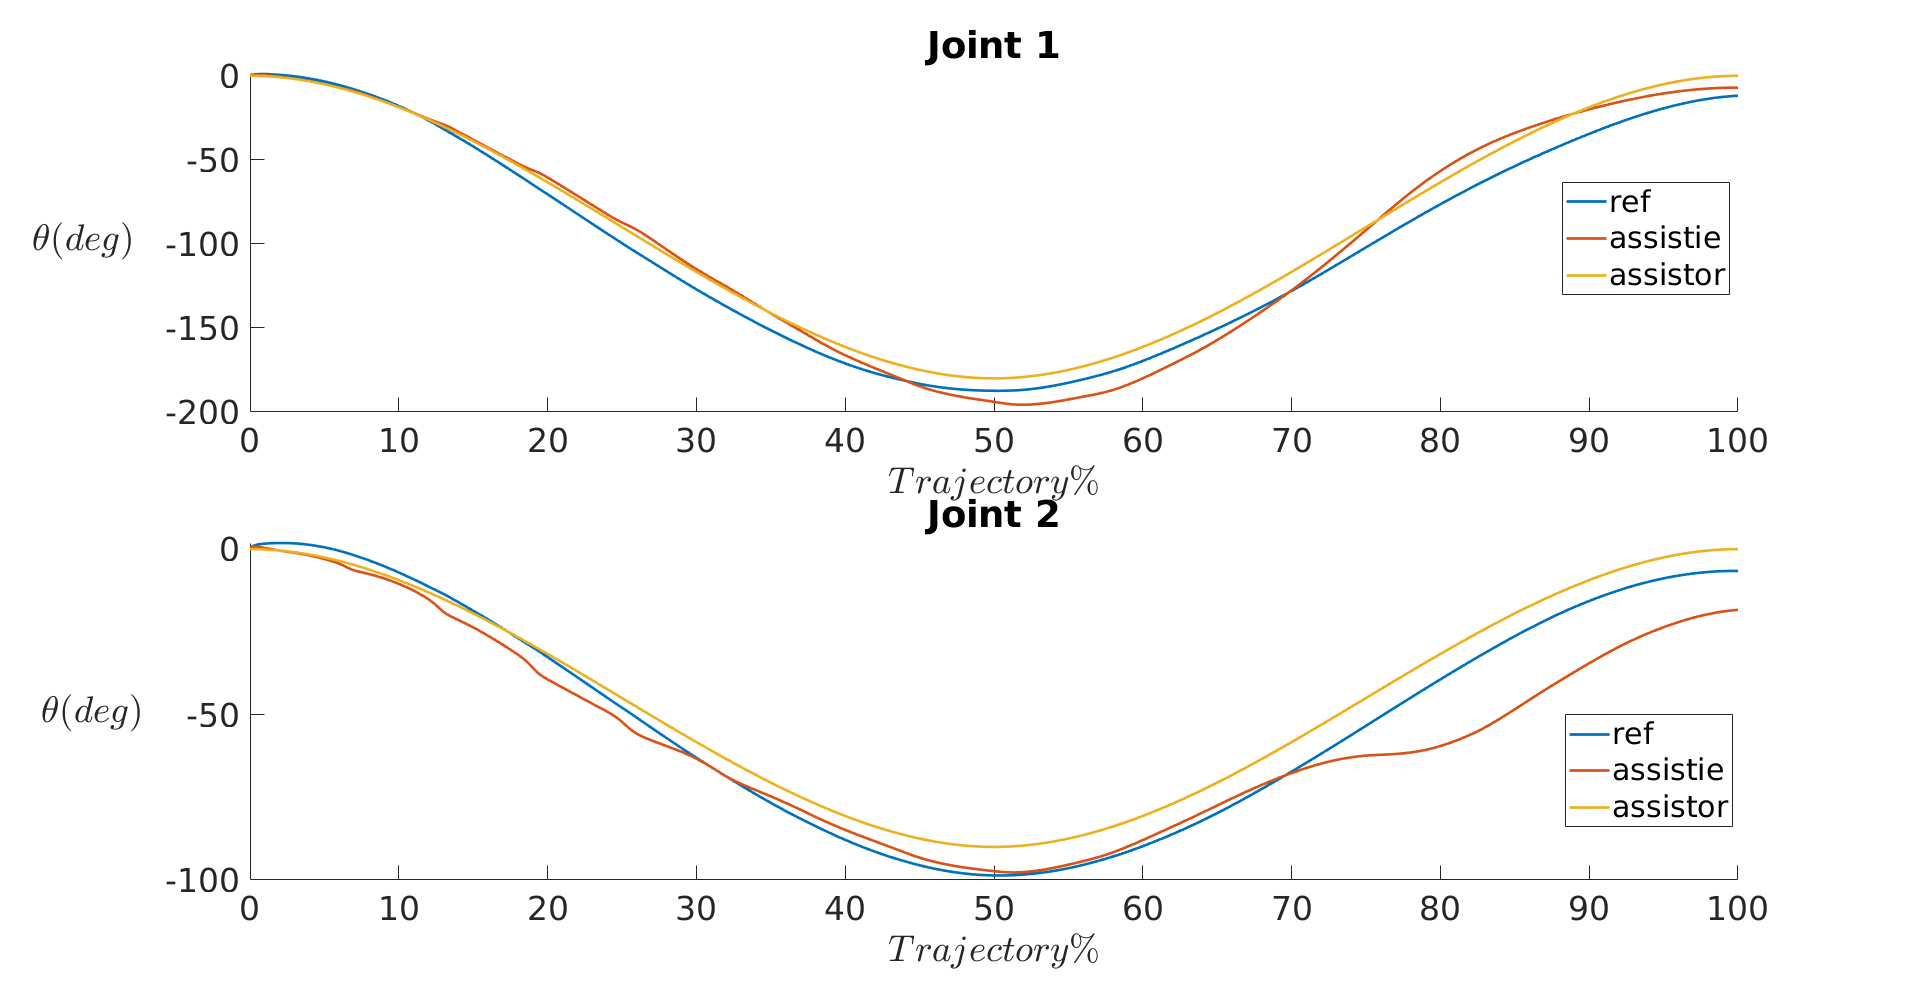
\includegraphics[width=\linewidth]{images/controllers/small_length_traj.png}
        \caption[Double Pendulum: Negative Alignment-Trajectory]{Trajectories of double pendulum}
        \label{fig:small_length_traj}
    \end{subfigure}
    \caption[Double Pendulum: Negative Alignment]{Double Pendulum model responses with at 0.95x of the human length \textit{assistie} torques.}
    \label{fig:small_length}
\end{figure}

\begin{figure}[h]
    \centering
    \begin{subfigure}{0.5\textwidth}
        \centering
        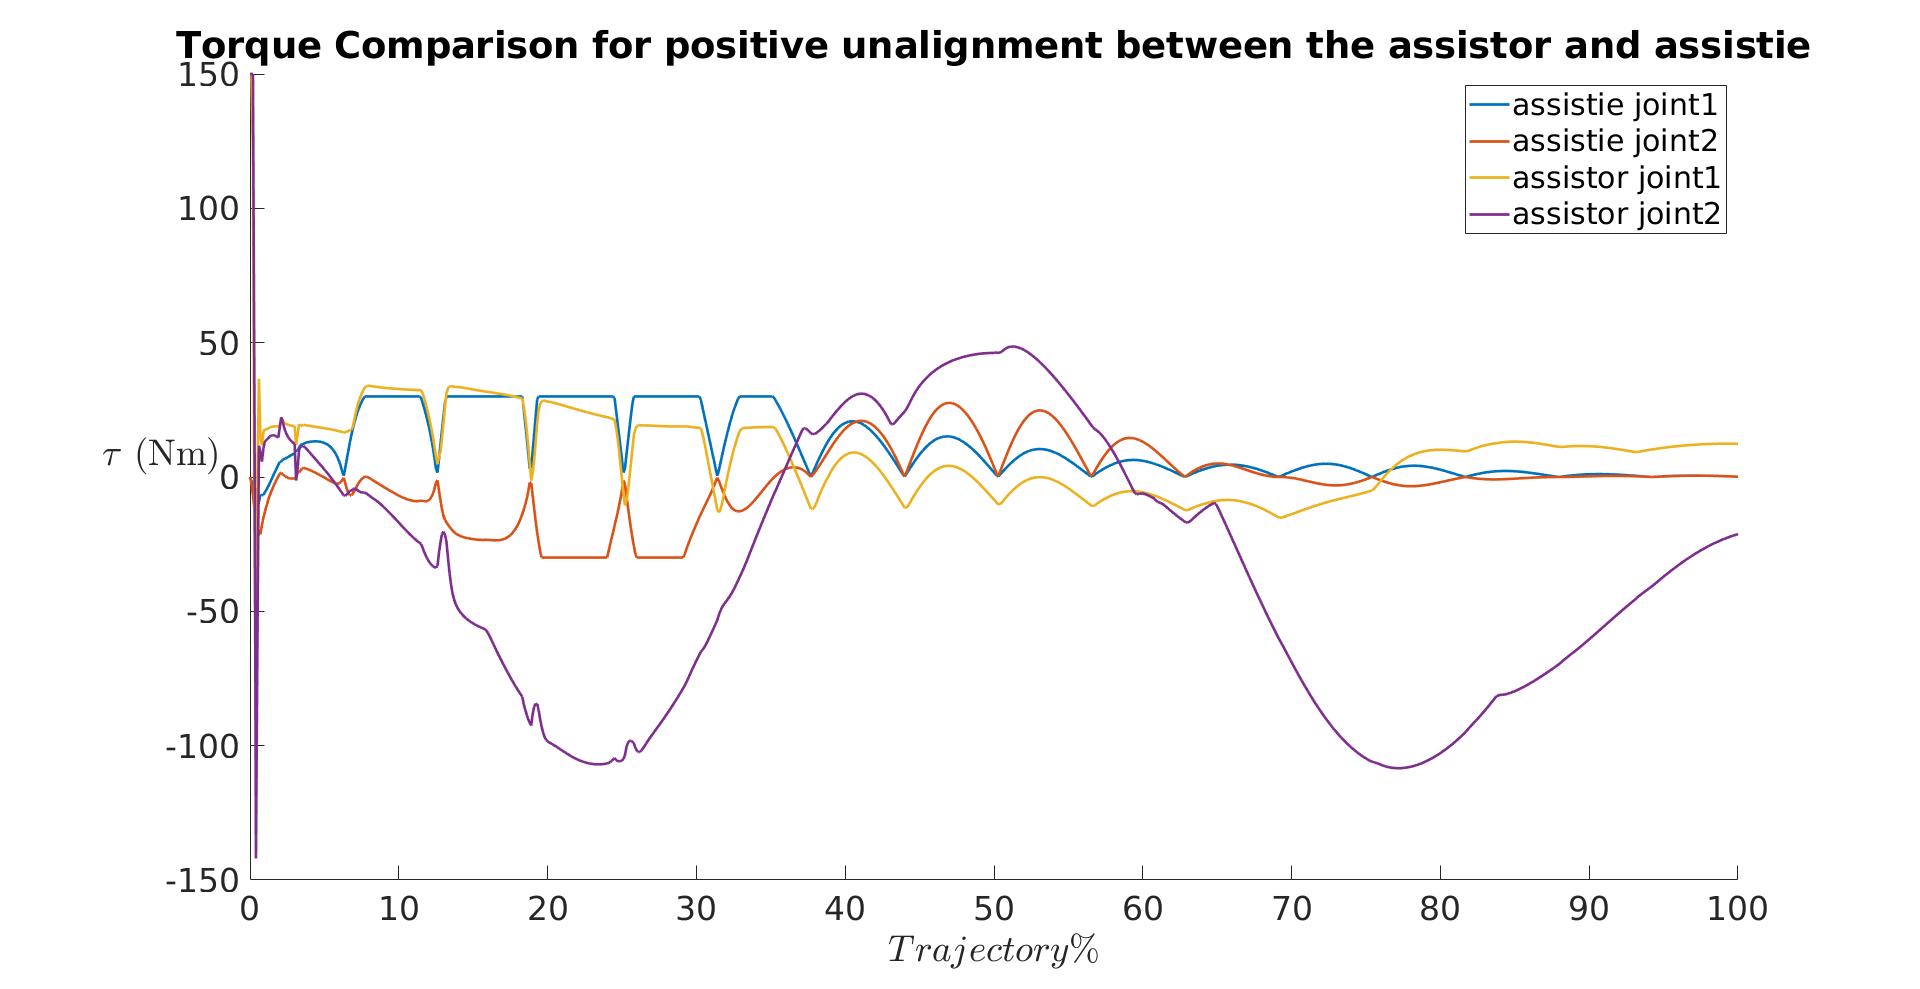
\includegraphics[width=\linewidth]{images/controllers/larger_length_torque.png}
        \caption[Double Pendulum: Positive Alignment-Effort]{Torque applied to the double pendulum}
        \label{fig:small_length_torque}
    \end{subfigure}%
    ~
    \begin{subfigure}{0.5\textwidth}
        \centering
        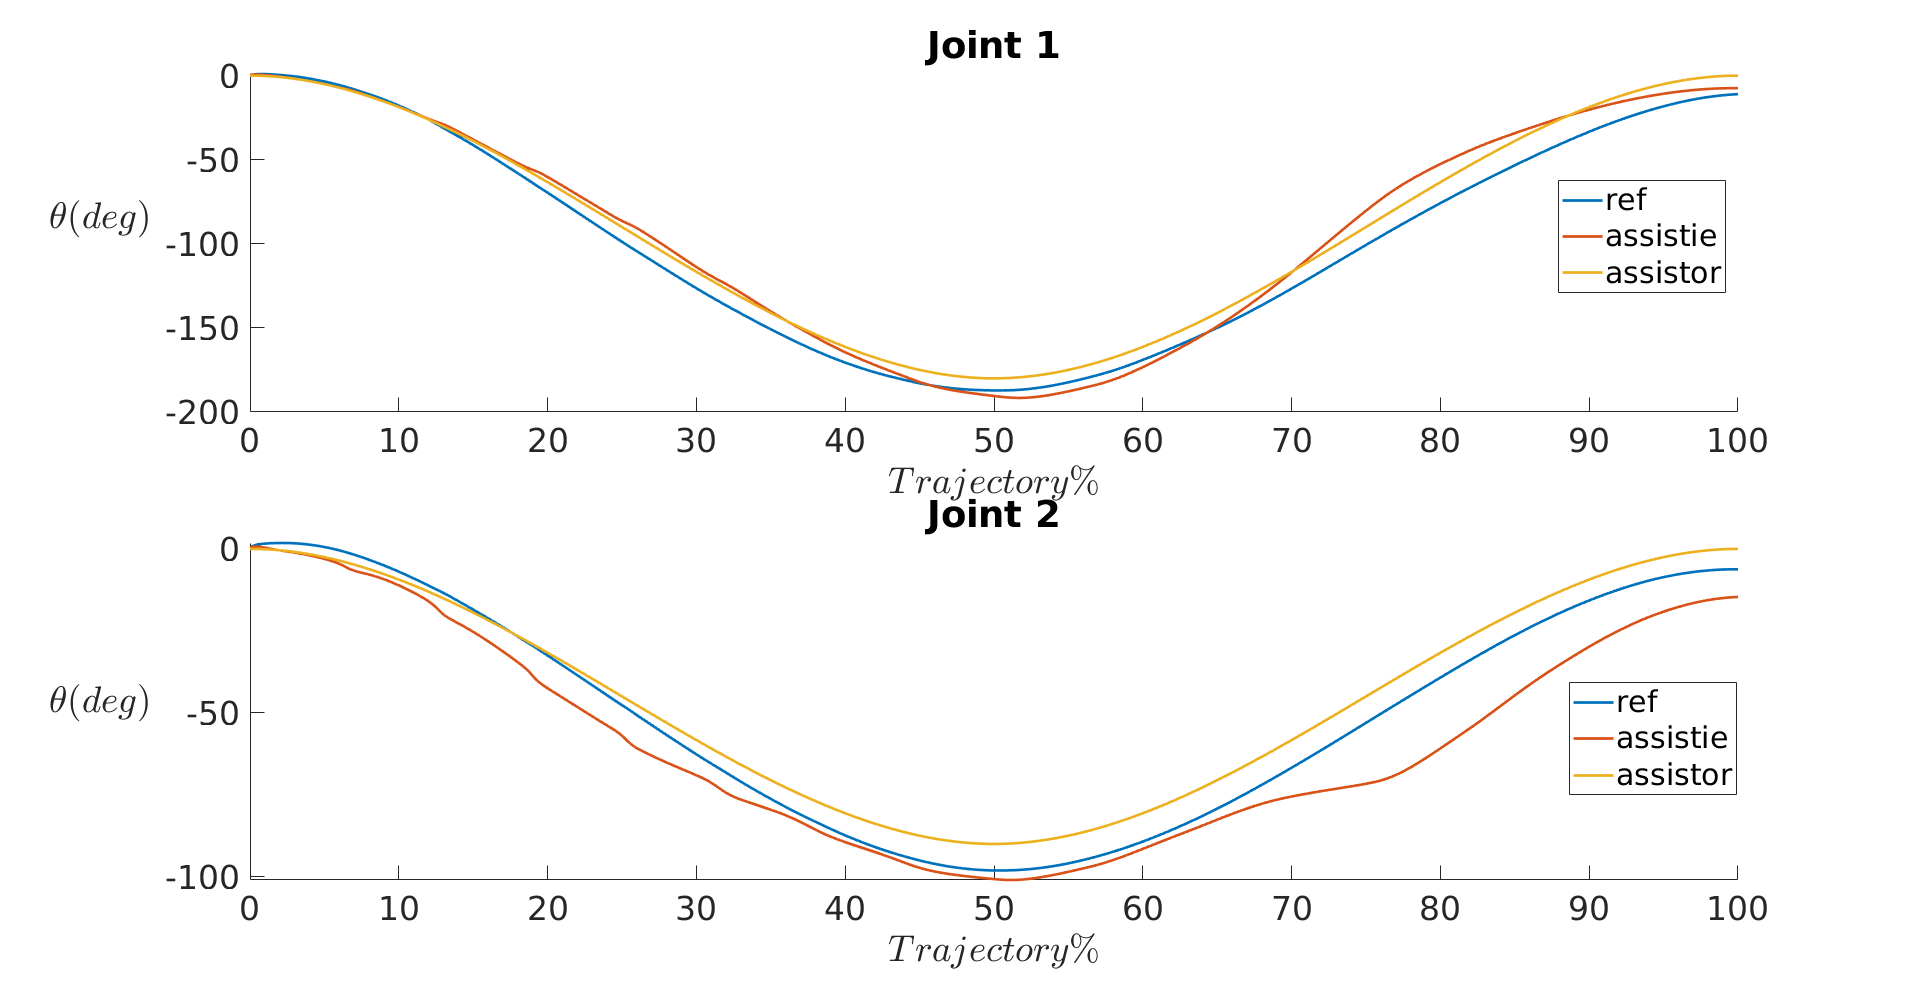
\includegraphics[width=\linewidth]{images/controllers/larger_length_traj.png}
        \caption[Double Pendulum: Positive Alignment-Trajectory]{Trajectories of double pendulum}
        \label{fig:small_length_traj}
    \end{subfigure}
    \caption[Double Pendulum: Positive Alignment]{Double pendulum model responses with at 1.05x of the human length \textit{assistie} torques.}
    \label{fig:larger_length}
\end{figure}


The controller performance increased by tuning the parameters of the SMC controller. The non-optimal parameters should have a significant deviation from the sliding surface. Using a cost function that considers velocity only has nearly the identical performance as the cost function that used both position and velocity; both performed better than the position only cost function. Using these results allows the velocity or the position and velocity to be good metrics for a cost function to tune the parameters of the A-SMC controller. The results show the importance of using the correct cost function to tune the controller gains. By selecting the wrong criteria for the tuning controller parameters, the controller will produce unstable results. It is important to note that the admittance controller parameters must be tuned in addition to the parameters of the SMC. If the variability parameters are too large, the admittance controller will lag/lead aggressively and not track the desired motion. 

\autoref{tab:error} summarizes the RMSE in degrees of the joint angles of the \textit{assistie} and \textit{assistor} systems. The largest error was caused with no  \textit{assistie} involvement. This is presumably caused by the non-rigid connection between the  \textit{assistie} and \textit{assistor} systems. The A-SMC controller does not have an understanding of the current state of the \textit{assistie} system, so it cannot directly control the position. However, since this was done in simulation, the error can be presented for comparison. The Spring-Dampener connection between the systems causes the \textit{assistie} to lag behind the \textit{assistie} system. Despite the \textit{assistie} it still only has an RSME error of $18.2^{\circ}$ on joint 1 and $16.7^{\circ}$ on joint 2; this is confirmed by examining the joint error of the reduced and time-varying simulations. The reduced test had the smallest RMSE, and the time-varying RMSE was between reduced and no-involvement simulations. The RMSE error should be within acceptable margins of error for a gait controller. The errors between the two systems, exoskeleton and human, can be reduced with a more rigid connection between the \textit{assistie} and \textit{assistor} systems which will have two effects on the system. First, the two systems will have smaller differences in position; this means that the \textit{assistie} or \textit{assistor} system will not lag or lead behind each other. Second, this will reduce the interaction force between the two systems. By increasing the stiffness between the two systems, the connection becomes more rigid, making the difference in the pose negligible and thus reducing the interaction force. On a real system, this can be achieved with form-fitted and tighter straps between the exoskeleton and the human.    


Testing the variability in alignment allows for testing of the controller when the systems are not perfectly aligned. This problem arises for real systems where the person's joints may not align perfectly with the exoskeleton joints. As shown \autoref{fig:small_length} and \autoref{fig:larger_length} the tracking signals were close to the time-varying signals with only a slight variation in the tracking RMSE.


\begin{table}[h!]
\centering
 \begin{tabular}{||c |c c c c||} 
 \hline
    involvement  & \textit{assistor J1} & \textit{assistor J2} & \textit{assistie J1} & \textit{assistor J2}\\ [0.5ex] 
 \hline\hline
 None & 5.9^{\circ} & 9.5^{\circ} & 18.2^{\circ} & 16.7^{\circ} \\ 
 Reduced & 8.4^{\circ} & 6.3^{\circ} & 7.8^{\circ}  & 5.2^{\circ}\\
 Time Varying & 9.6^{\circ} & 6.2^{\circ} & 10.3^{\circ}  & 9.6^{\circ}\\ 
 0.95x length & 9.9^{\circ} & 6.6^{\circ} & 10.0^{\circ}  & 9.4^{\circ}\\
 1.05x length & 9.3^{\circ} & 6.3^{\circ}  & 10.7^{\circ}   & 9.8^{\circ}  \\[1ex] 
 \hline
 \end{tabular}
 \caption[Joint RMSE for Double Pendulum]{Joint RSME (Degrees) of the double pendulum system}
  \label{tab:error}
\end{table}





\subsection{Application of Tuning Methodology on a Simple Trajectory}

The tuning methodology discussed above was implemented on a leg of the LARRE using the dynamics server to calculate the inverse and forward dynamics. This new system is illustrated in \autoref{fig:LegModel}. 


\begin{figure}
    \centering
    \begin{subfigure}{0.5\textwidth}
        \centering
        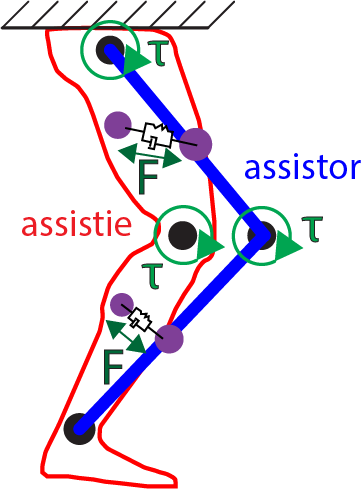
\includegraphics[width=0.75\linewidth]{images/controllers/leg.png}
        \captionsetup{width=.8\linewidth}%
        \caption[Leg Model used for Optimization and Control]{Leg Model used for Optimization and Control. Here the black circle are the joint  location and the purple circle are the center of masses. The shown location does not represent the actual center of mass or joint locations.}
        \label{fig:LegModel}
    \end{subfigure}%
    ~
        \begin{subfigure}{0.5\textwidth}
        \centering
        \includegraphics[width=0.75\linewidth]{images/controllers/strap_springs.png}
        \captionsetup{width=.8\linewidth}%
        \caption[LARRE with strap positions]{Location of the LARRE's straps on the person. The straps allow for slight movement between the exoskeleton and the person.}
        \label{fig:strappositions}
    \end{subfigure}
    \caption[Connection between LARRE and the person]{Connection between the person and the LARRE and the associated dynamic model.}
    \label{fig:my_label}
\end{figure}




The tuning method discussed above was used to tune the controller. Each of the leg joints was commanded to follow a polynomial trajectory; this allowed for the boundary conditions of the path to be controlled for testing. This model added complexity to the tuning process since it added another dimension that needed to be tuned. An assumption was made that while the thigh and shank of the exoskeleton were connected via a spring-dampener system, the foot of the exoskeleton and human were rigidly connected as shown in \autoref{fig:strappositions}. Additionally, the closed-loop PD controller is assumed to be an FES type device that can transform displacement into torque through pulse width and frequency modulation \cite{rouhani2017pid, ha2015approach,Model_Ferrarin}. The hip and knee joints of the exoskeleton controller are assumed to be powered by BLDC motors as discussed in \autoref{chap:mech}.

\autoref{fig:LARRE_TUNING} shows the cost convergence over the optimization. A single leg was tuned to lower the number of parameters needed to be optimized. The optimization lowers the RSME cost from 2.66 to 0.6, a 77.44\% reduction. At each step in the iterations, the parameters are changed in an attempt to lower the cost function. The parameters being tuned have different magnitudes and are thus graphed separately to show the change at each step accurately. \autoref{fig:LARRE_Train_Trajectory} compares the output of the training model to the desired trajectories. As shown, the initial starting position has some wobbling in the ankle position for the training model, which converges to the desired trajectory. The wobbling can be due to the initial conditions in the admittance controller or the value of $\lambda$ being too large, which affects the rise time.  

\begin{figure}
    \centering
    \begin{subfigure}[b]{\textwidth}
        \centering
        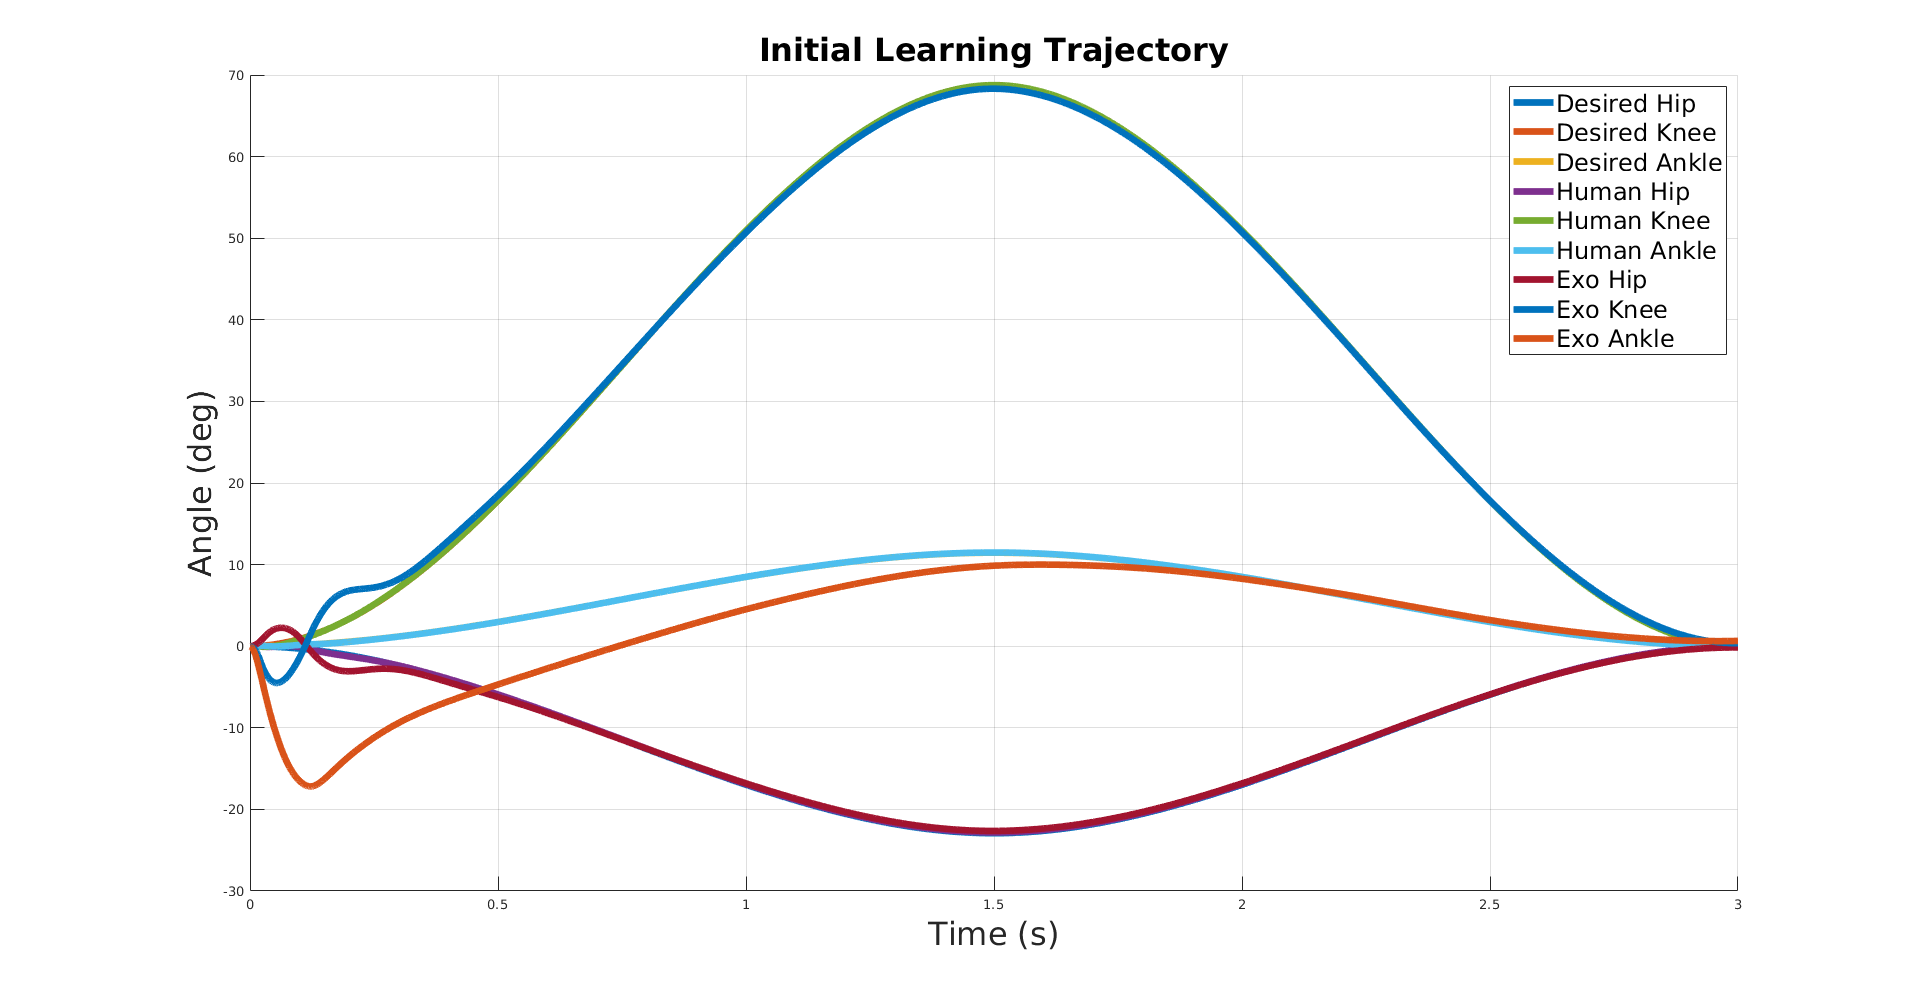
\includegraphics[width=0.75\columnwidth]{images/controllers/trajs/init_traj.png}
        \caption[LARRE Training Trajectory]{A single simple trajectory used as a training trajectory. The dynamic and kinematic model of LARRE was used for training. }
        \label{fig:LARRE_Train_Trajectory}
    \end{subfigure}
    
    \begin{subfigure}[b]{\textwidth}
        \centering
        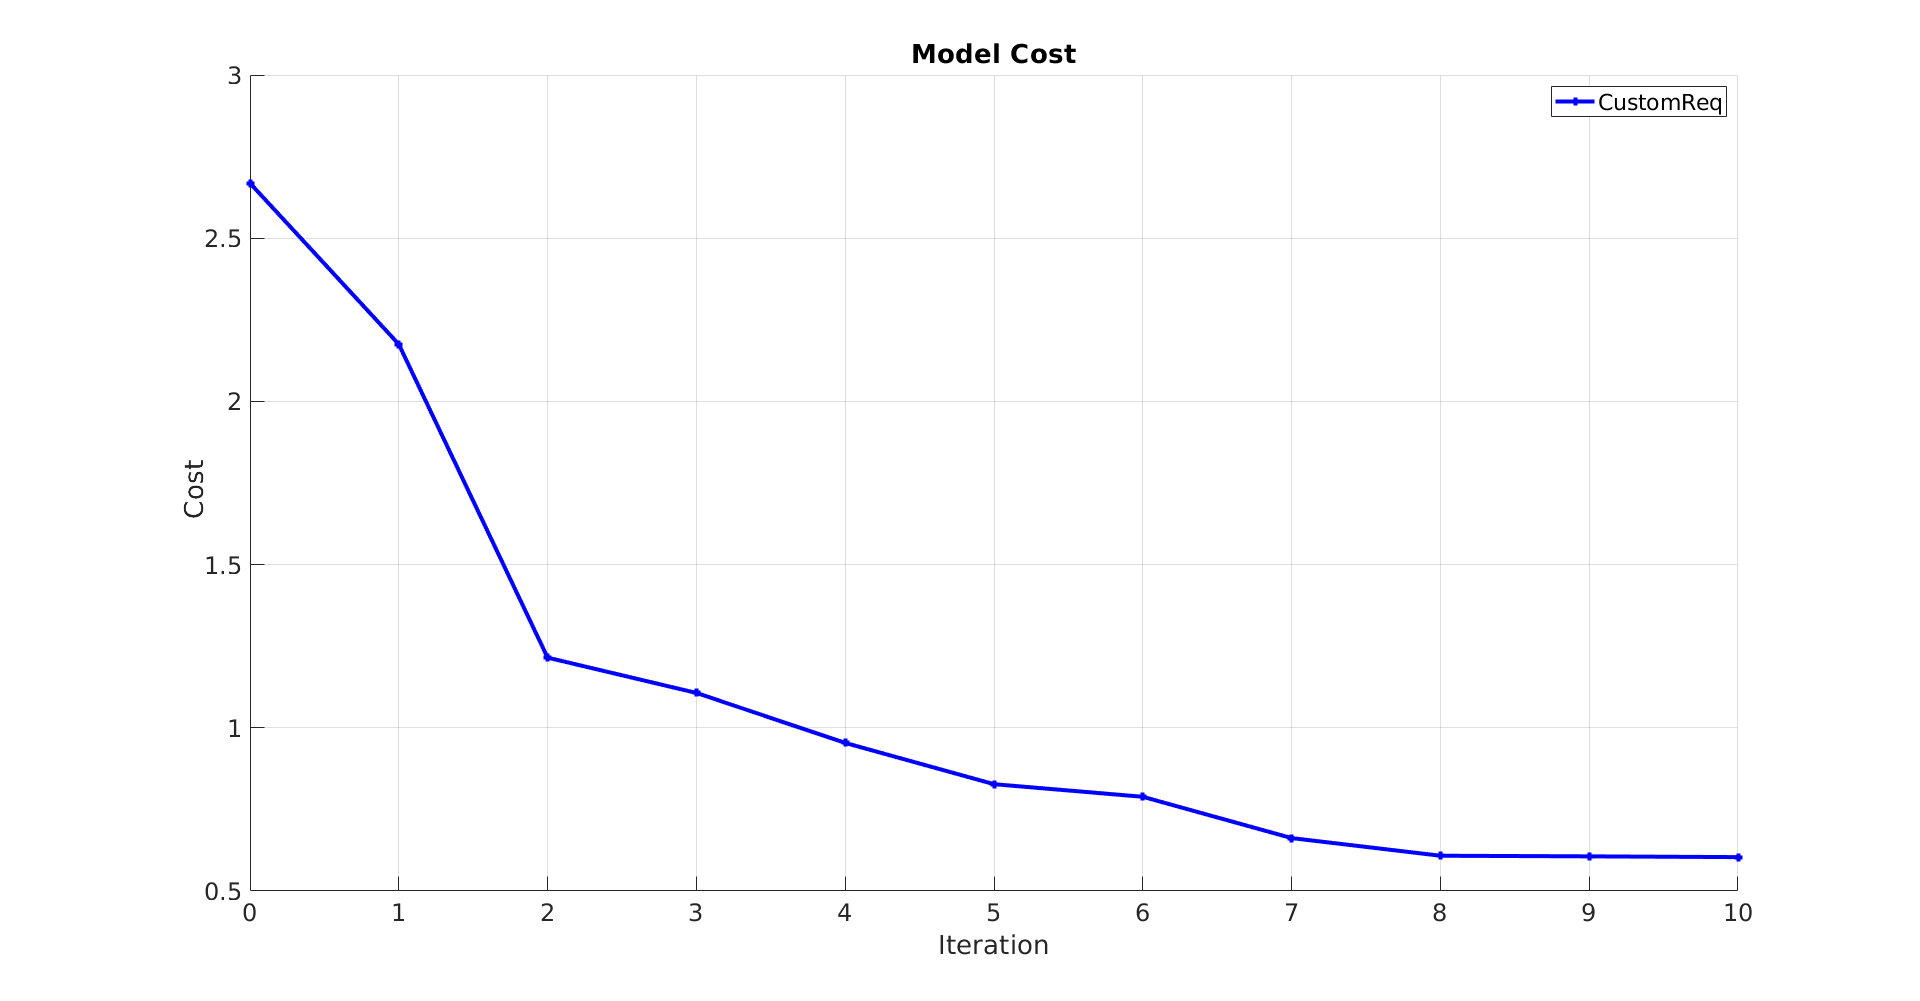
\includegraphics[width=0.75\columnwidth]{images/controllers/trajs/cost.png}
        \caption[LARRE Cost Optimization]{Cost of Tuning a single leg of LARRE. The cost converges after approximate 10 iterations. }
        \label{fig:LARRE_TUNING}
    \end{subfigure}
  
    \begin{subfigure}[b]{\textwidth}
        \centering
        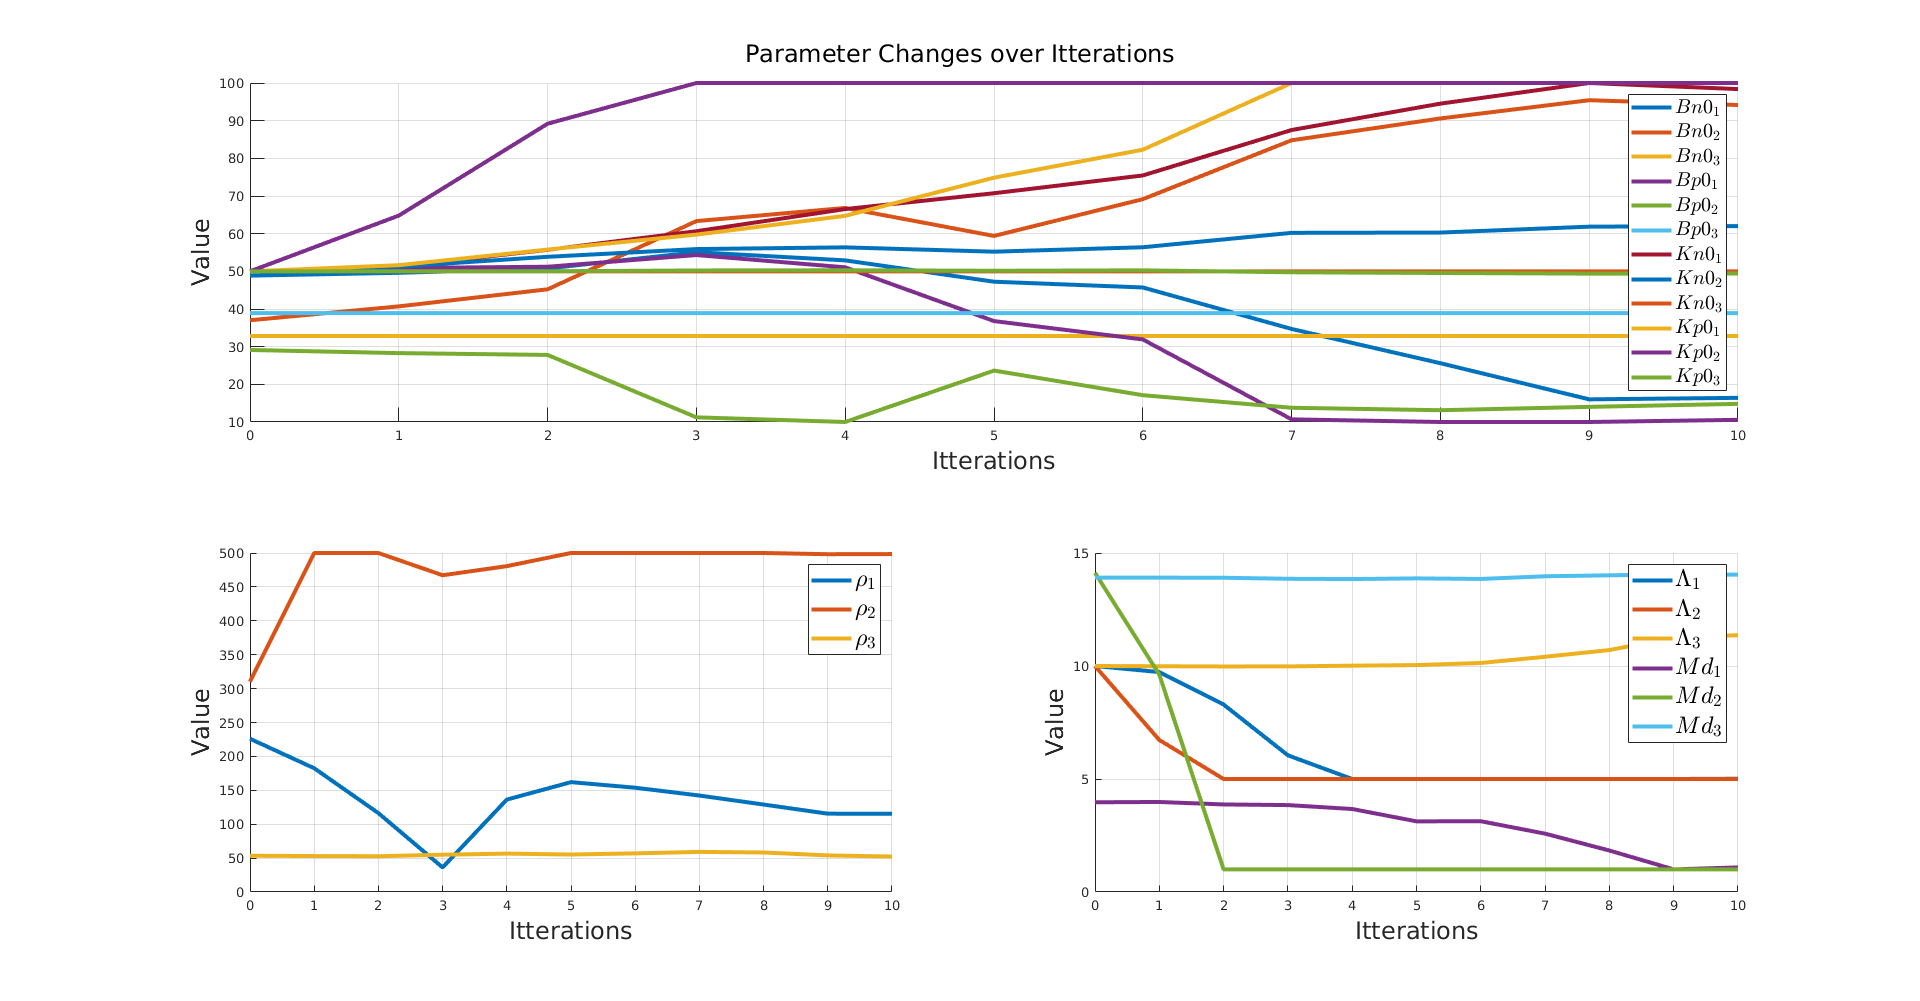
\includegraphics[width=0.75\textwidth]{images/controllers/trajs/params_splite.png}
        \caption[LARRE Parameters Optimization]{Parameters Changing Over Iterations. The values are separated into three graphs due to the different magnitude of the parameters.}
        \label{fig:LARRE_PARAMS}
    \end{subfigure}

    \caption{Output for Training LARRE Graphs}
    \label{fig:traj_training_graph}
\end{figure}


While \autoref{fig:LARRE_PARAMS} shows how the parameters change over time, it does not give insight into the relative importance of the tuning parameters. A global sensitivity analysis was done to examine which parameters have the most significant effect on the cost function. The goal of the analysis is to apportion the uncertainty in outputs to the uncertainty. A global sensitivity analysis is when all the parameters are varied simultaneously over the entire range of the inputs factors \cite{saltelli2008global}; this can be done by examining several different correlation methods listed below. Additionally, these methods can also be examined as \textit{Ranked} methods. A ranked correlation method measures an ordinal association between the different variables. The ranking is the assignment of the ordered labels. 

\begin{itemize}
    \item \textbf{Correlation}: Statistical relationship between two variables. 
    \item \textbf{Kendall}: Measure the ordinal association between two measured quantities \cite{abdi2007kendall}.
    \item \textbf{Standardized Regression}: A regression analysis where the underlying data is standardized so the variance of dependence can be compared \cite{SIEGEL2016355}.  
    \item \textbf{Partial Correlation}: Measures the degree of association between two random variables, with the effect of a set of controlling random variables removed \cite{PARTIALCORRELATION}. 
\end{itemize}




\autoref{fig:paramStats} shows the relative importance of the parameters; here, the graphs are defined between -1 and 1. The closer the value is to $\|1\|$, the higher its sensitivity. As the parameter approaches 1, the cost function will increase; the cost function will decrease as the parameter approaches -1. 

This data can be used to choose the more important parameters when optimizing the system; this is important for systems with many parameters. Examining the results indicates that the variable $M_d$ has little impact on the cost function. This low impact is expected since the $M_d$ variable is a constant post multiplier the $K_d$ and $B_d$ terms (see \autoref{eq:addmittance}-\autoref{eq:varible}). The relatively high importance of $\rho$ can be explained by its effect on the A-SMC. The $\rho$ is with the sliding mode gains, which controls the chattering in the system as shown in \autoref{eq:SMCChattering}, where $T_s$ is the time, and $\Delta$ is the chattering. The $\alpha$ parameter controls how the variable admittance controller reacts. Changes to this variable will impact the value of the $Kn$ and $Kp$ gains, which have relatively high importance controlling the torque to generate a difference in position between the two systems; if the two systems drift apart, the controller increases the gain to align the systems. In contrast, the $Bn$, $Bp$, and $\gamma$ terms have relatively low importance, indicating that the two systems generally had the same velocity, so increasing the gains had little effect on the system. 



\begin{equation}
    \Delta = \rho T_s
    \caption[A-SMC Chattering]{A-SMC Chattering}
    \label{eq:SMCChattering}
\end{equation}


\begin{figure}
    \centering
    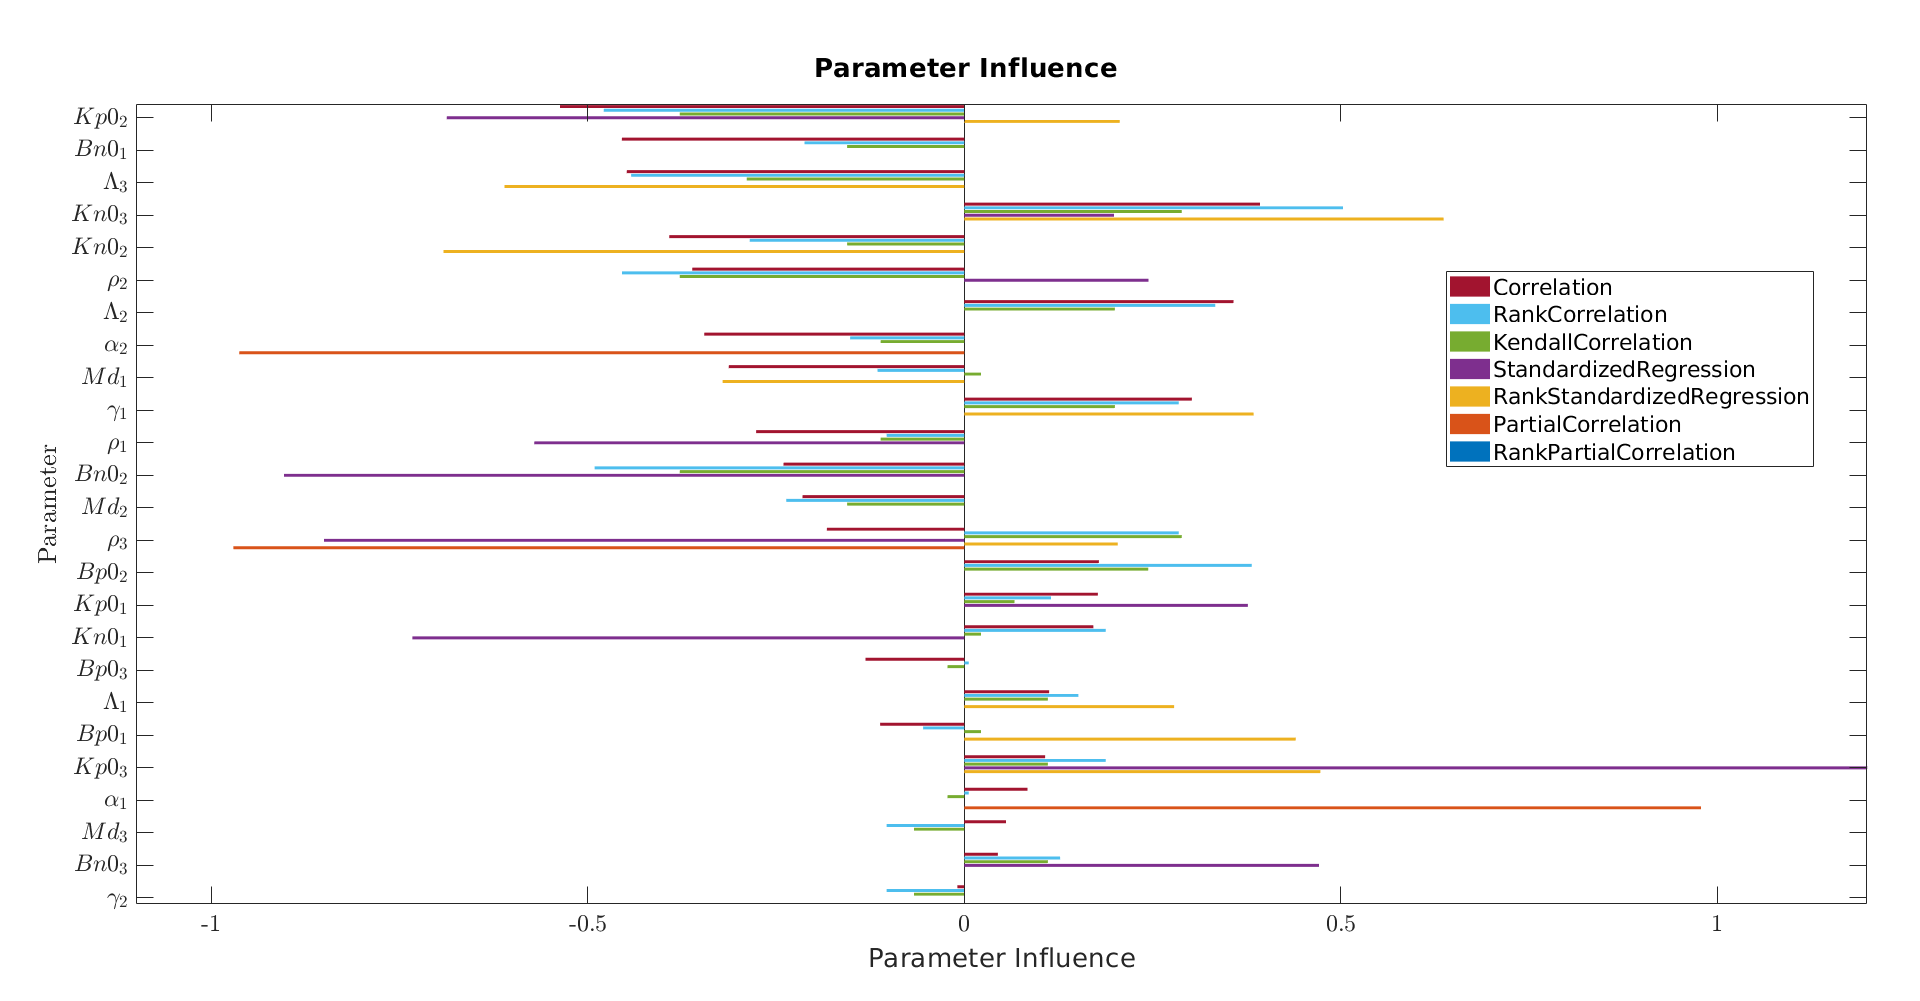
\includegraphics[width=\columnwidth]{images/controllers/trajs/stats.png}
    \caption[Relative Parameters Importance]{Comparison of relative parameters importance of the A-SMC. The larger the line the more sensitivity the parameter as on the cost function. }
    \label{fig:paramStats}
\end{figure}



The effect of the model gains and the controller's ability to adapt to varying human interactions were examined. The same trajectory was repeated three times to show the steady-state behavior of the controller. Additionally, the foot is omitted since it is considered to be rigidly attached to the exoskeleton foot. 
The effects of the human effort were applied to the system from full human interaction to zero human interaction were examined, including 80\% involvement, 50\% involvement, 20\%, and a time decaying involvement. The percentage involvement was defined by examining the torque generated at 100\% involvement, approximate $10Nm$. 

\autoref{fig:StateSpaceTrajectory} shows the state space of the hip and knee joint. They show that the joints move towards the sliding surface and converge towards zero with minimal chattering. As shown in \autoref{fig:TripleTrajectory} the initial start part of the trajectory takes some time to settle to the trajectory. After the initial part of the motion, it settles. The hip motion is slightly off the desired motion. 



\begin{figure}
    \centering
    \begin{subfigure}{\linewidth}
        \centering
        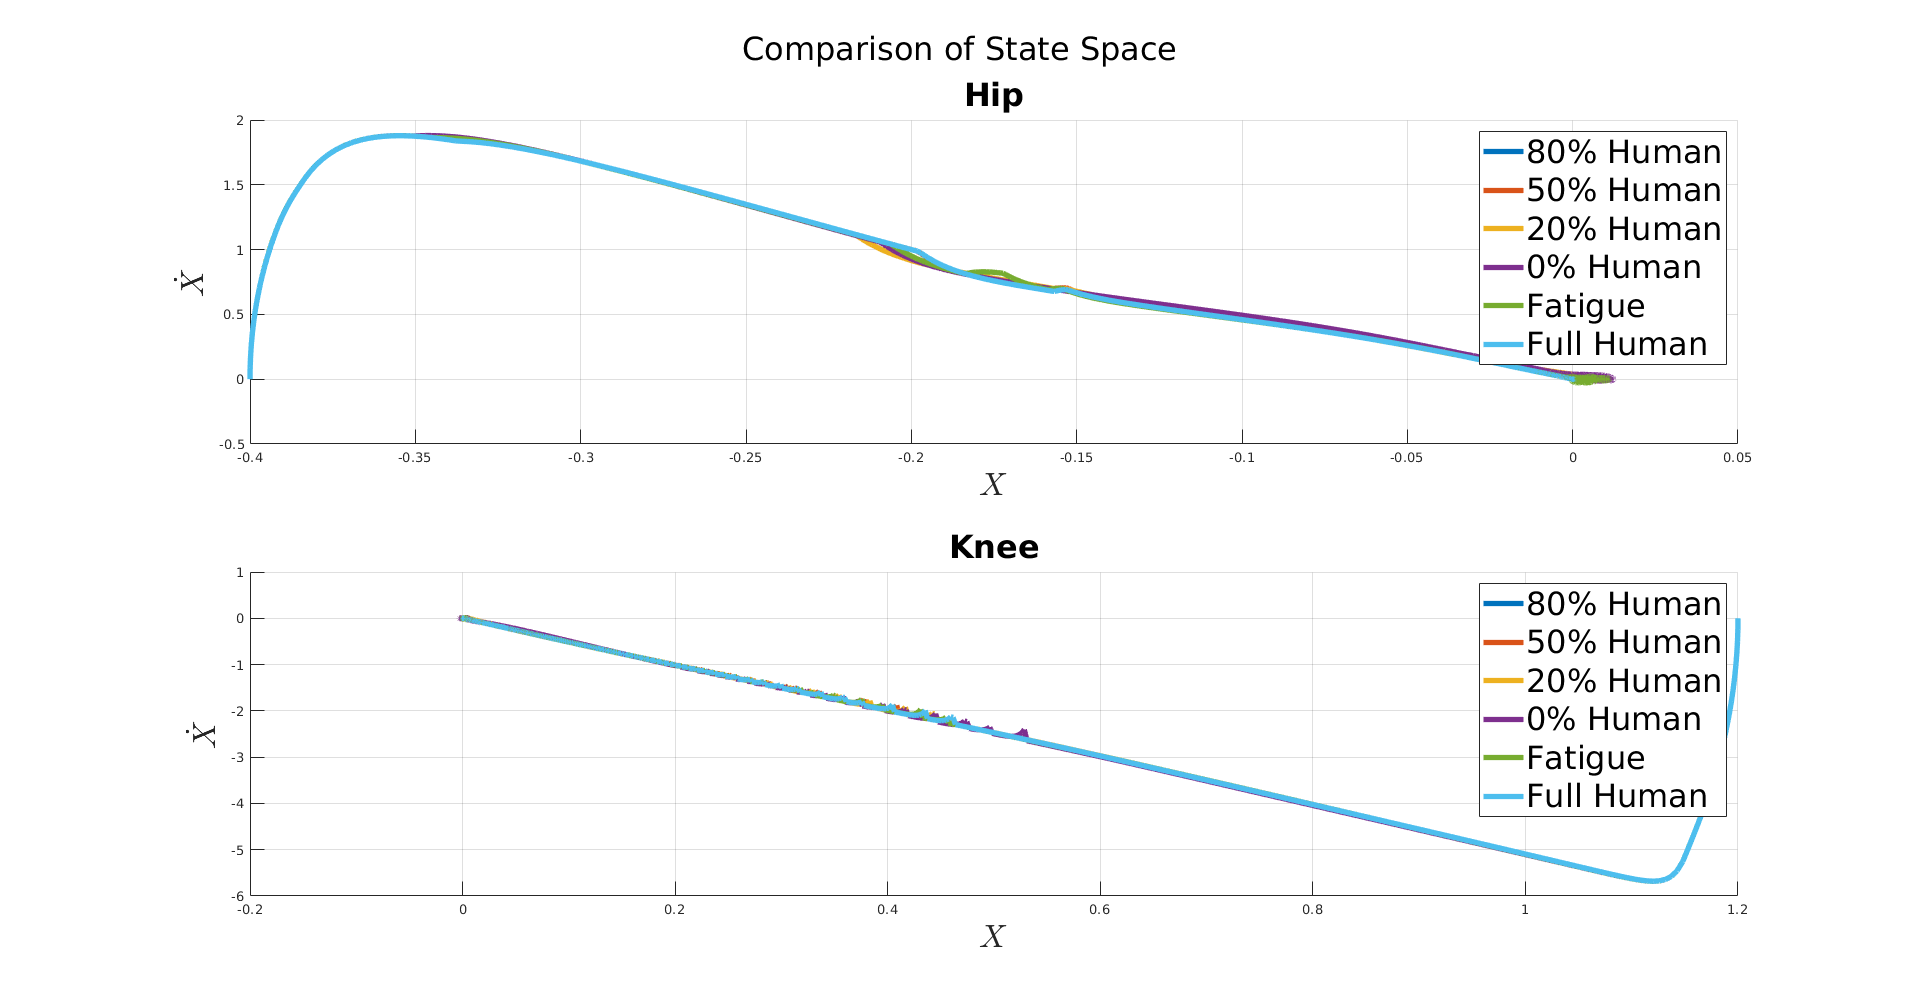
\includegraphics[width=\columnwidth]{images/controllers/trajs/statespace.png}
        \caption[State Space Trajectory]{Comparison of state space trajectory at different engagement levels.}
        \label{fig:StateSpaceTrajectory}
    \end{subfigure}
    \begin{subfigure}{\linewidth}
        \centering
        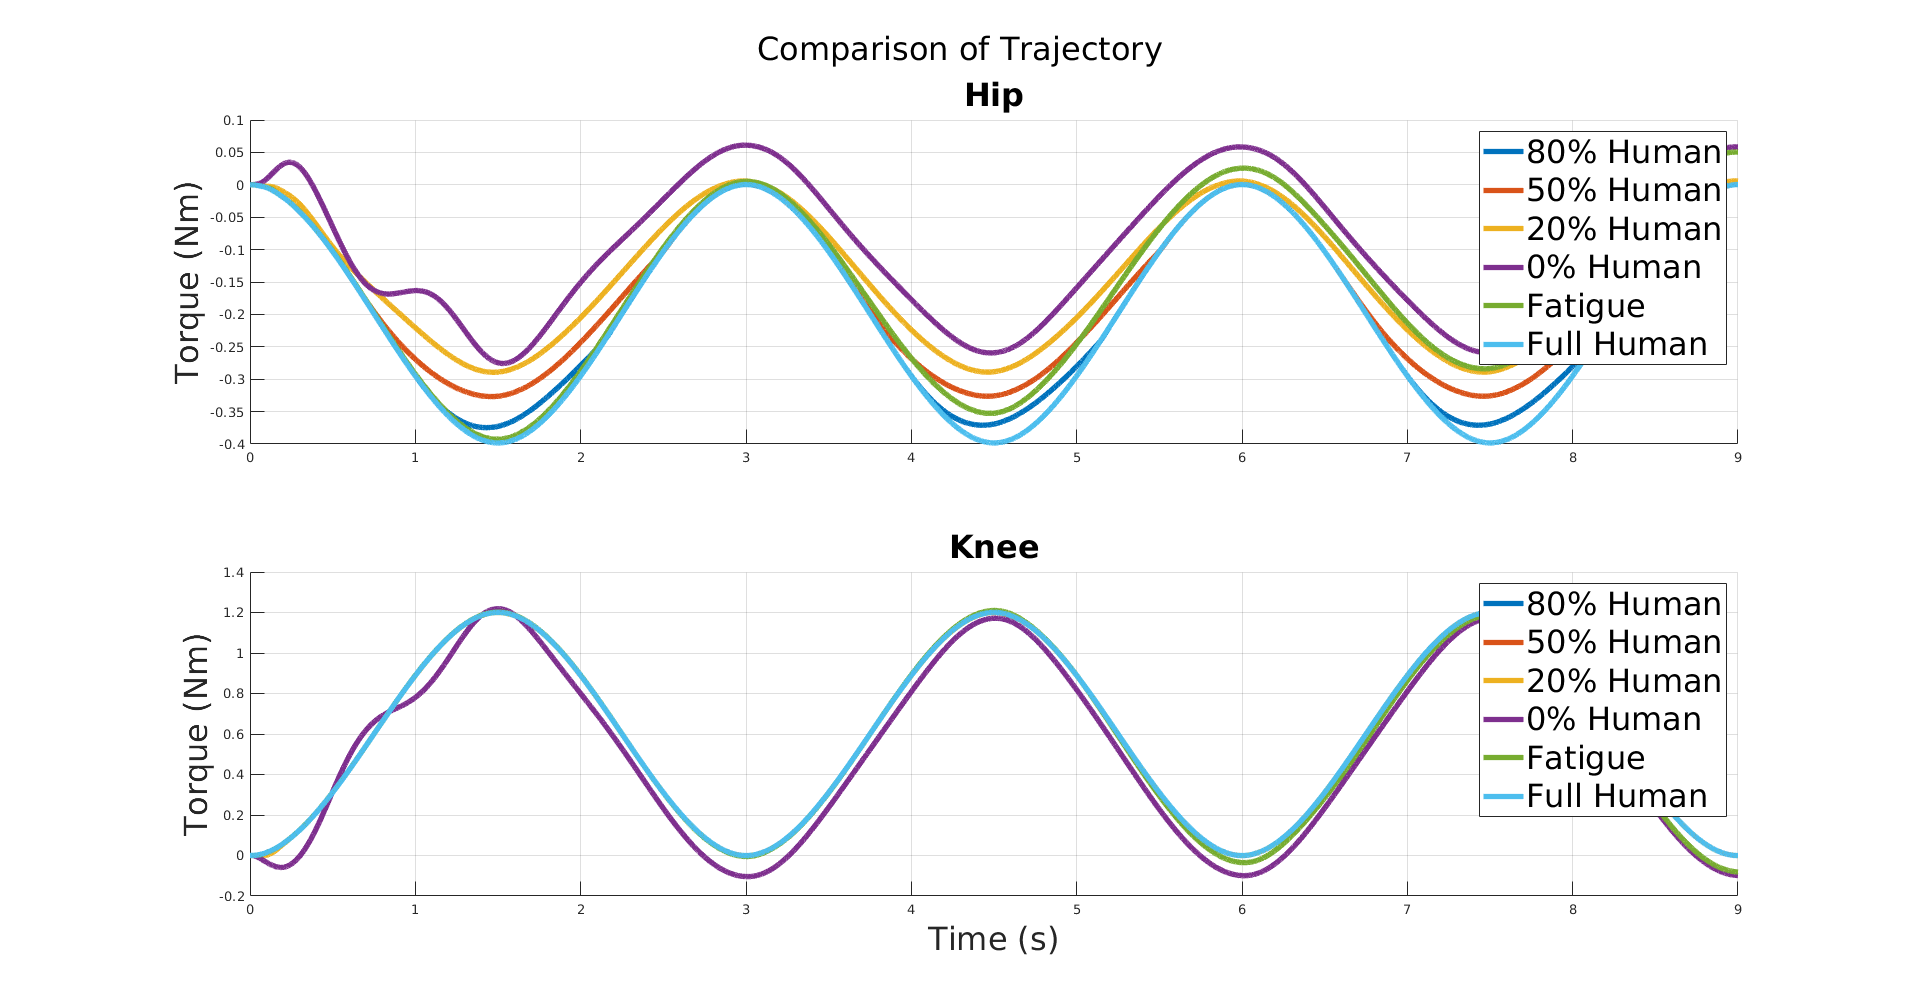
\includegraphics[width=\columnwidth]{images/controllers/trajs/triple_traj.png}
        \caption[Triple Trajectory]{Comparison of a simple triple trajectory at different engagement levels}
        \label{fig:TripleTrajectory}
    \end{subfigure}
    \caption[Triple Trajectory LARRE]{Comparison of a of simple triple trajectories applied to the system at different engagement levels.}
    \label{fig:TripleTraj}
\end{figure}



The human interaction is shown in \autoref{fig:humantripletraj}. The human effort was saturated for the varying interaction levels since the torque cannot exceed the capped value. The fatigue started at 80\% human interaction and reduced as an exponential sine wave to 0\% interaction as shown in \autoref{fig:fatprofile}. While this may not be an accurate model, it represents a decreasing torque over time. Additional fatigue is difficult to model as it depends on the patient's muscle atrophy, the muscle activated, and the pulse width used to activate the muscle \cite{reiner1998patient}. As expected, the fatigue interaction contains a wave-like motion as the PD controller attempts to handle the varying engagement levels. 


\begin{figure}
    \centering
    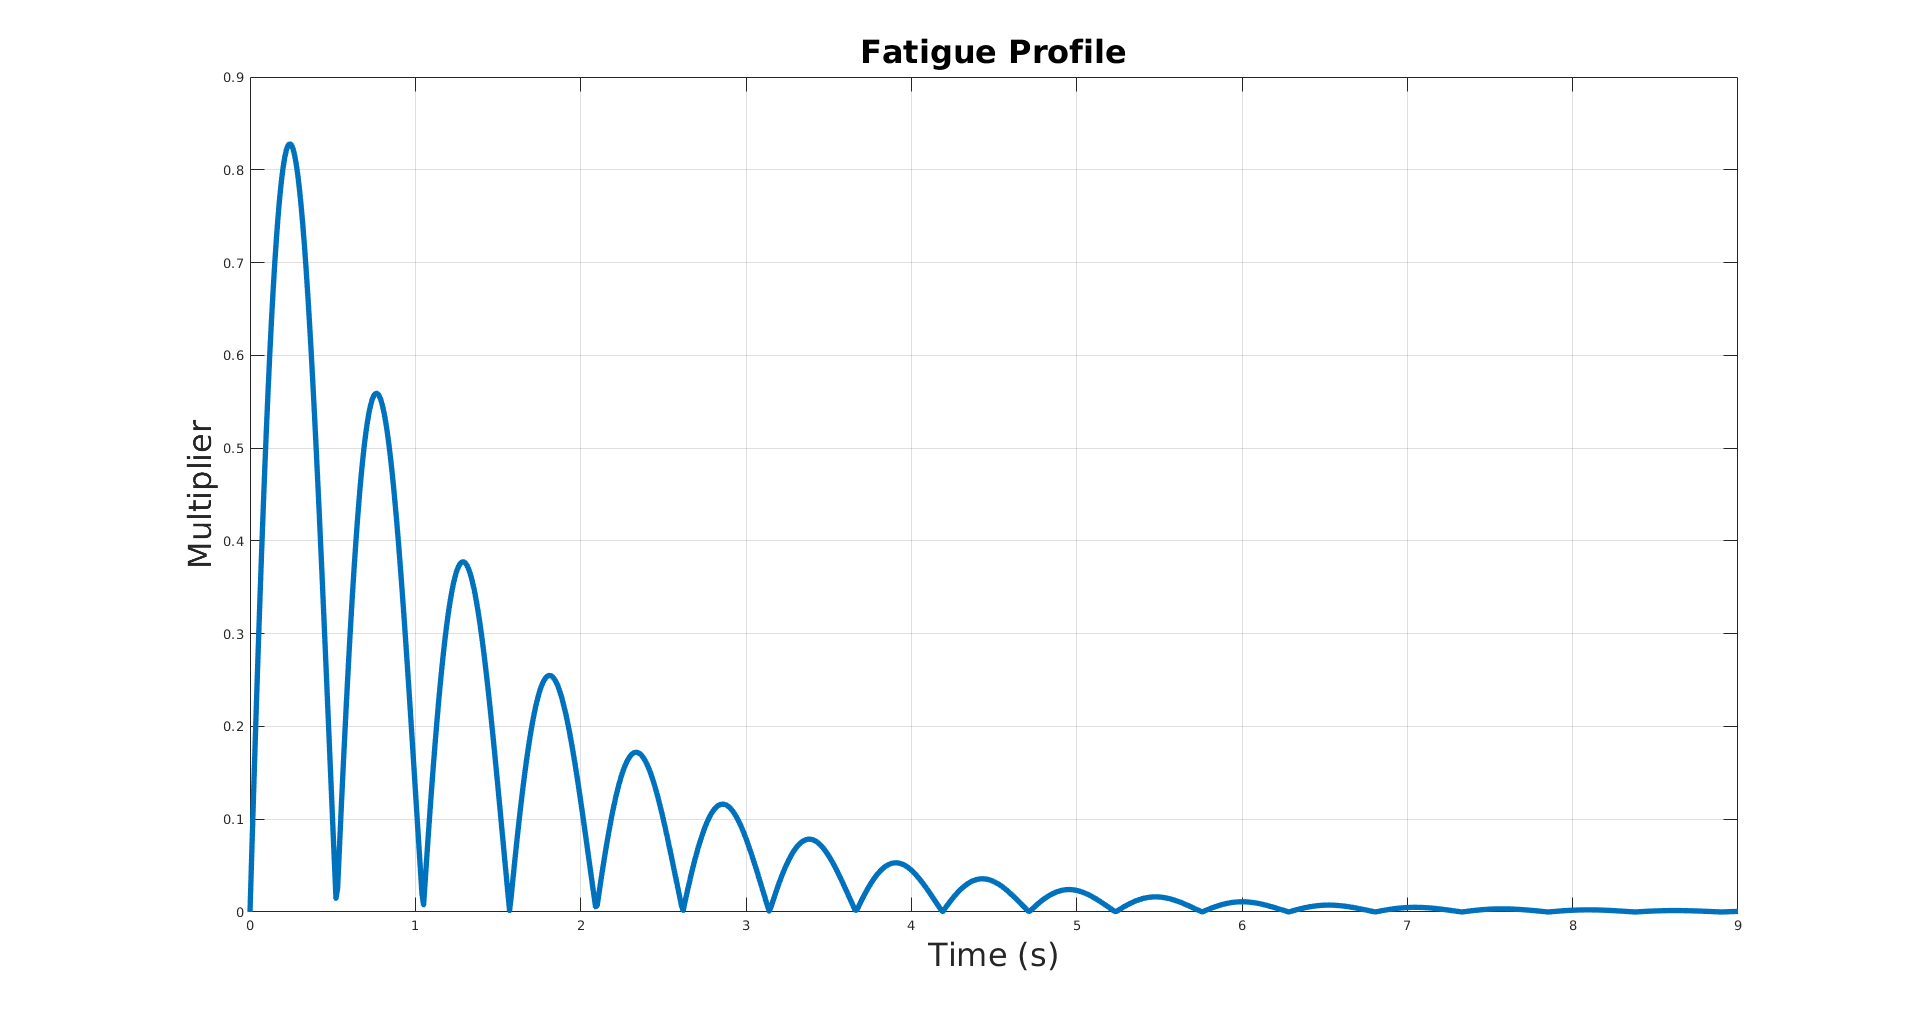
\includegraphics[width=\columnwidth]{images/controllers/gait/fat_profile.png}
    \caption[Fatigue Profile]{Fatigue Profile applied to the \textit{assistie} (human) torque. This is not a realstice fatigue profile but is mearly used to simulate both decay and change in magnitude.}
    \label{fig:fatprofile}
\end{figure}


\begin{figure}
    \centering
    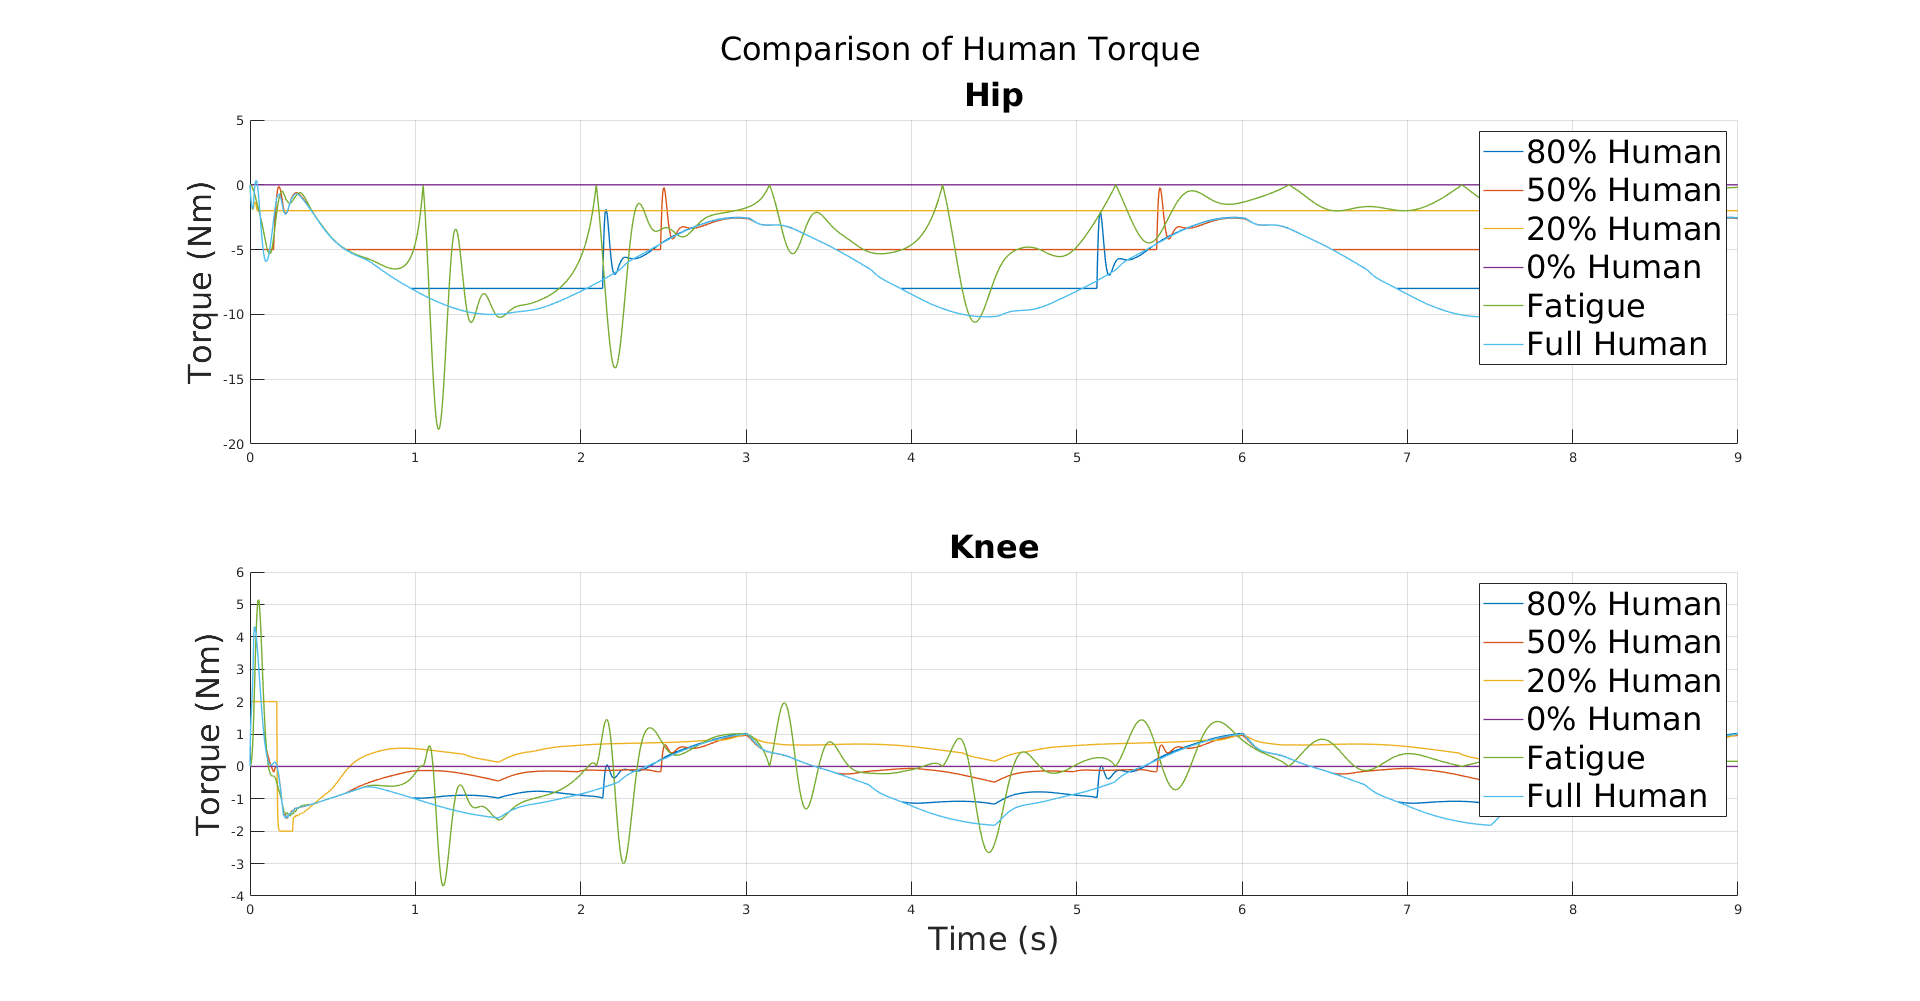
\includegraphics[width=\columnwidth]{images/controllers/trajs/human.png}
    \caption[Human Torque over Triple Trajectory]{Human Torque over Triple Trajectory}
    \label{fig:humantripletraj}
\end{figure}


\autoref{fig:SMCTripleFull} shows the effort supplied by the A-SMC for each of the engagement levels. \autoref{fig:SMCTripleZoom} is a zoom of the same graph. As shown, as the human engagement increased, the A-SMC magnitude of the effort decreased for both hip and knee joints; this shows that the A-SMC controller is adapting the human engagement level. 


\begin{figure}
    \begin{subfigure}{\linewidth}
        \centering
        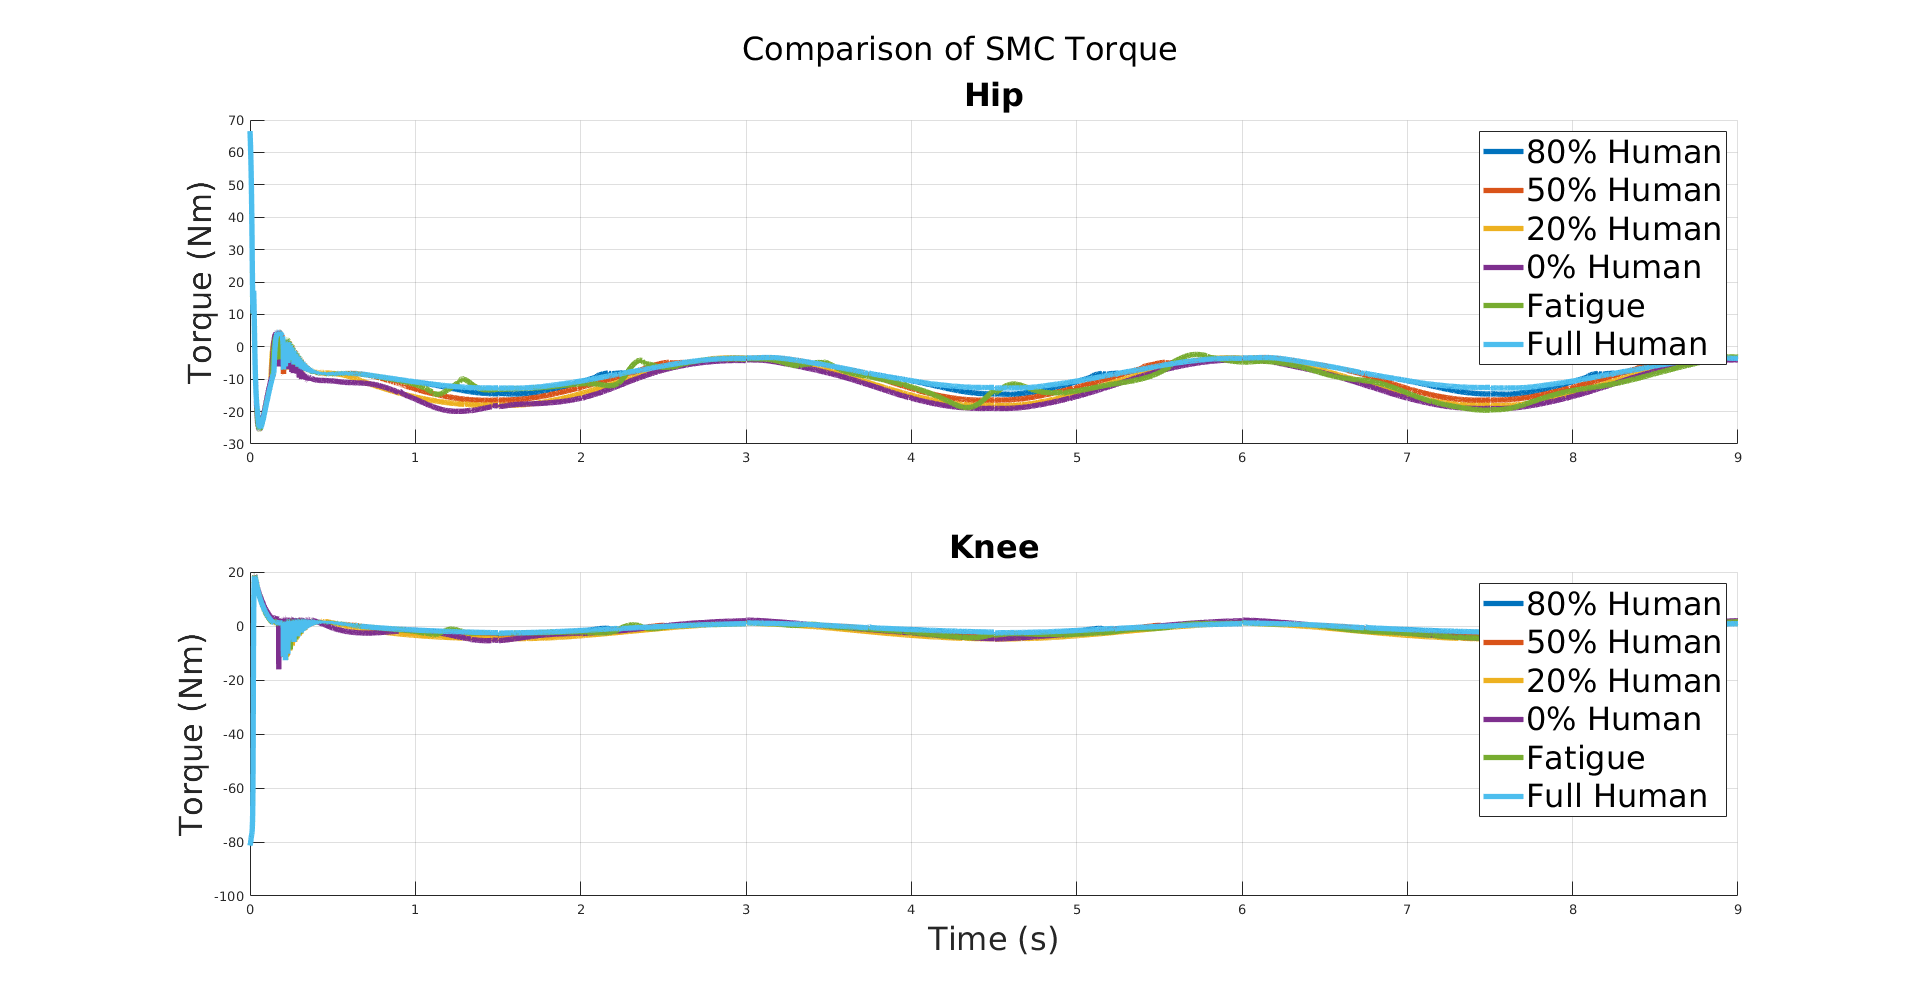
\includegraphics[width=\columnwidth]{images/controllers/trajs/SMC_full.png}
        \caption[A-SMC Torque over Triple Trajectory]{A-SMC Torque over Triple Trajectory}
        \label{fig:SMCTripleFull}
    \end{subfigure}
    \begin{subfigure}{\linewidth}
        \centering
        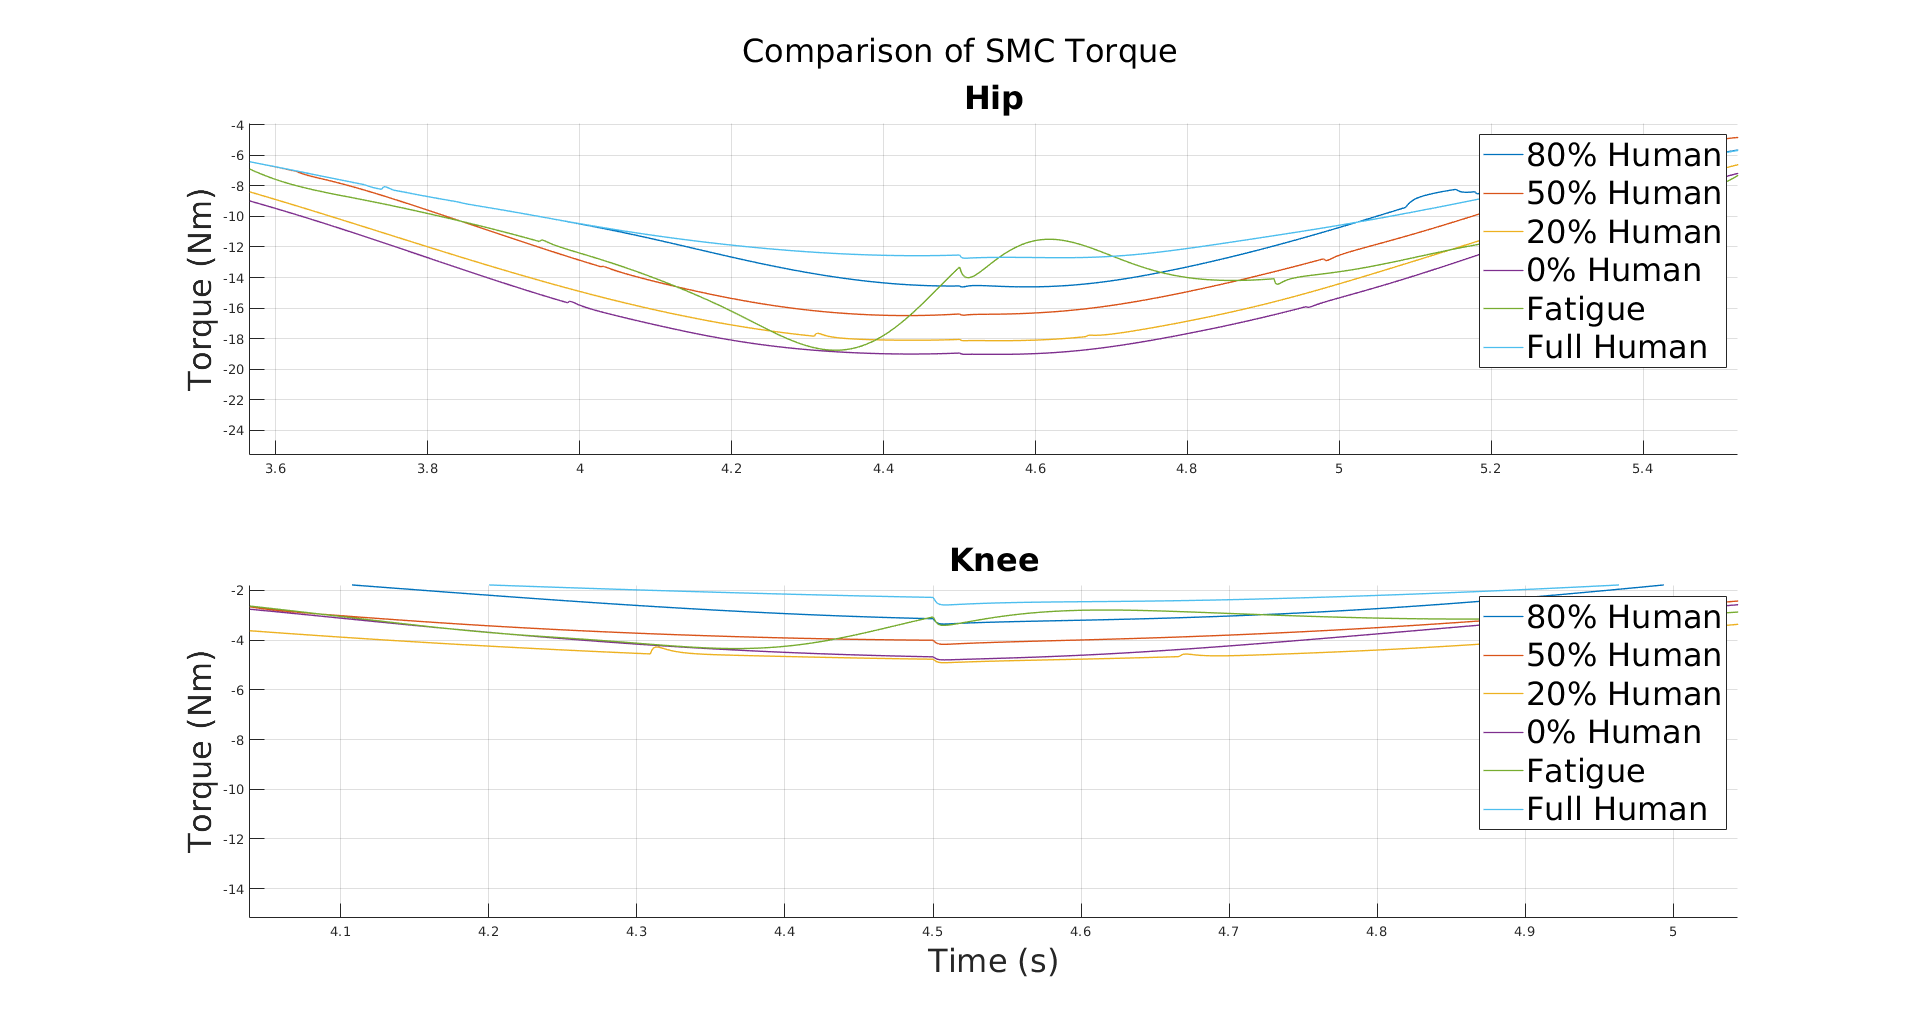
\includegraphics[width=\columnwidth]{images/controllers/trajs/SMC_zoom.png}
        \caption[A-SMC Torque over Triple Trajectory Zoomed]{A-SMC Torque over Triple Trajectory Zoomed In}
        \label{fig:SMCTripleZoom}
    \end{subfigure}
    \caption[A-SMC Effort applied over the Triple Trajectory]{A-SMC Effort applied over the Triple Trajectory. As shown the magnitude of the applied \textit{assistor} (A-SMC) effort decrees as the \textit{assistie} (human) engagement increases. }
    \label{fig:SMCEffortTriple}
\end{figure}

The interaction torques between the LARRE and the human provide the assistive torques. The spring-dampener systems generate the force, which is transformed in the torques. \autoref{fig:InteractionTripleTraj} shows the interaction trajectories, as expected, the magnitude interaction torque increases when then the human involvement decreases; this is because the human motion is lagging behind the location of the exoskeleton, thus generating larger forces. 

\begin{figure}
    \centering
    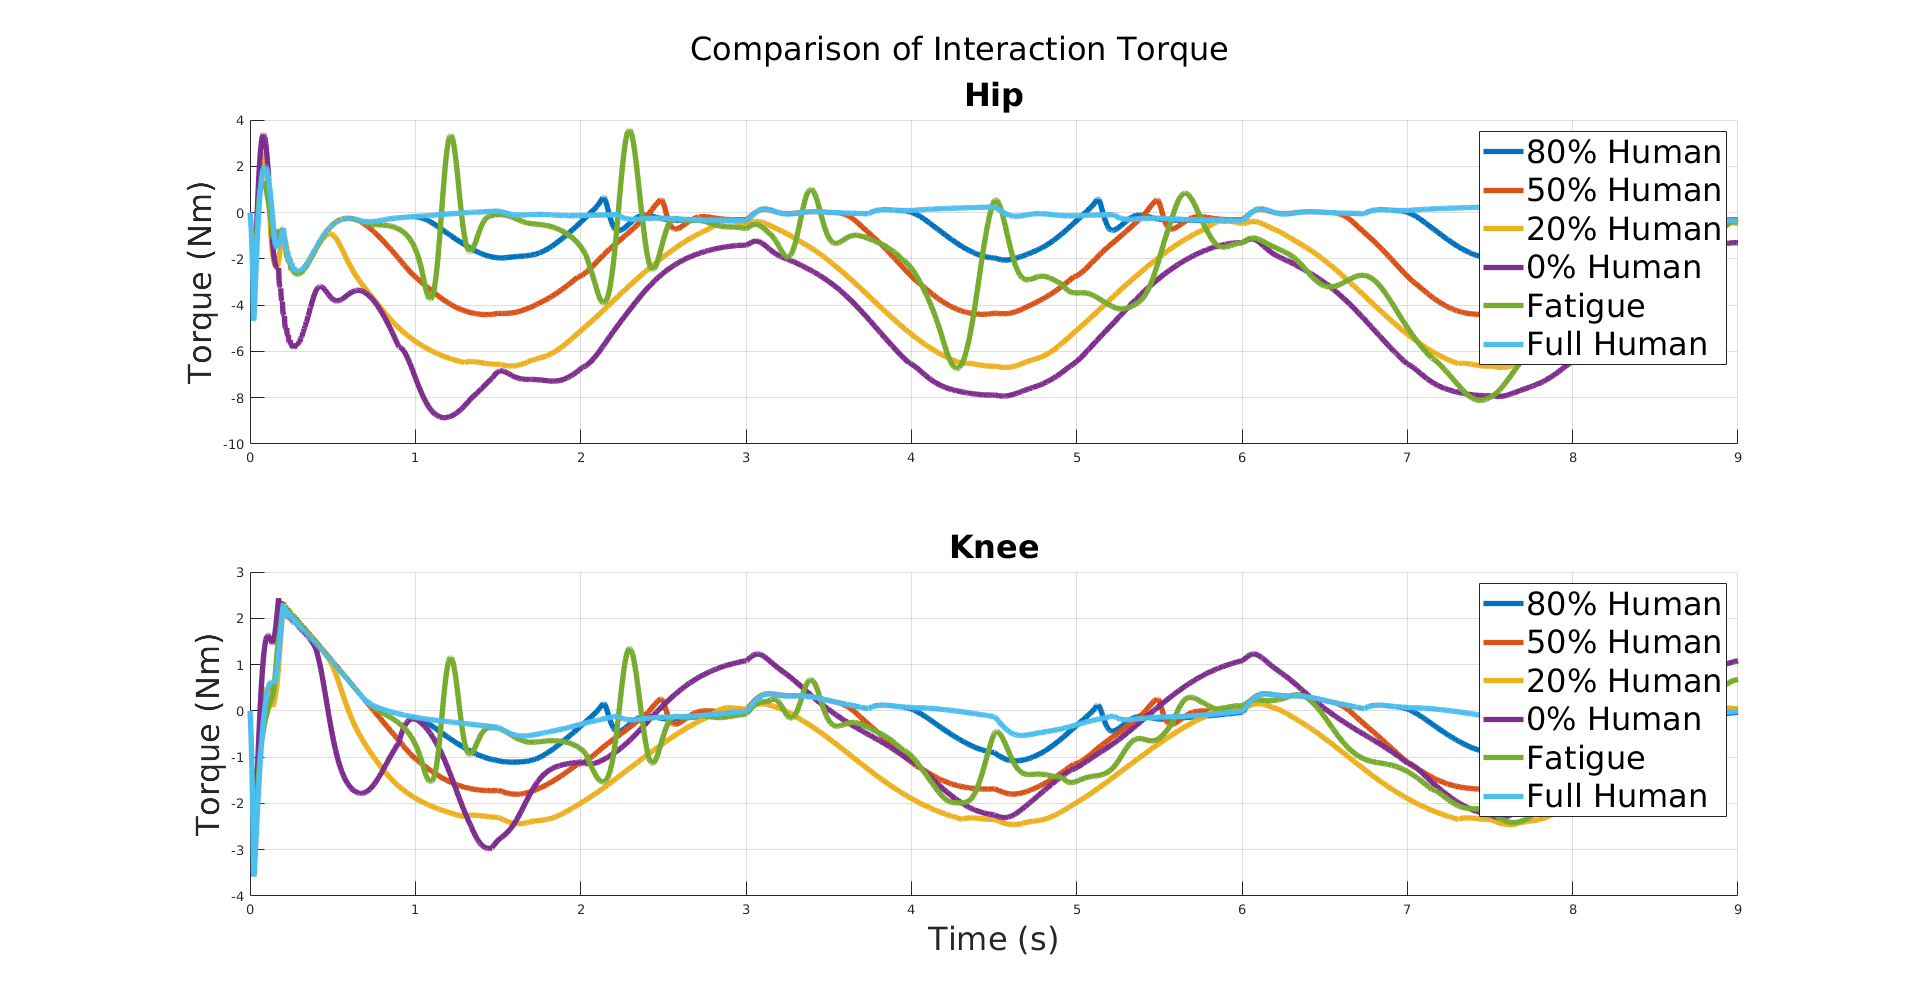
\includegraphics[width=\columnwidth]{images/controllers/trajs/interactions.png}
    \caption[Triple Trajectory Interaction Torques]{Triple Trajectory Interaction Torques}
    \label{fig:InteractionTripleTraj}
\end{figure}


\subsection{Application of Tuning Methodology to Follow a Gait Cycle}


The model was used to follow a three gait cycle to observe the steady-state motion of the controller using the parameters calculated above. The trajectory was auto-generated by combining three gait cycles. One of the key changes to the model was using the torques pre-calculated by the iLQR method (see \autoref{sec:ilqr}) as the standard interaction torques. Instead of using an inverse dynamic model, the iLQR controller should produce optimal torques to follow the gait trajectory. The A-SMC then compensates for the disturbances in the system. \autoref{fig:CoopSimulink} shows the Simulink model used to control the gait following model. The highlighted output torques are sent to the dynamics server, which double integrates the output to get the joint positions and velocity, which are fed back as the input joint states. The interaction dynamics are the spring-dampener equations that calculate the coupled forces.  



\begin{figure}[h!]
    \centering
    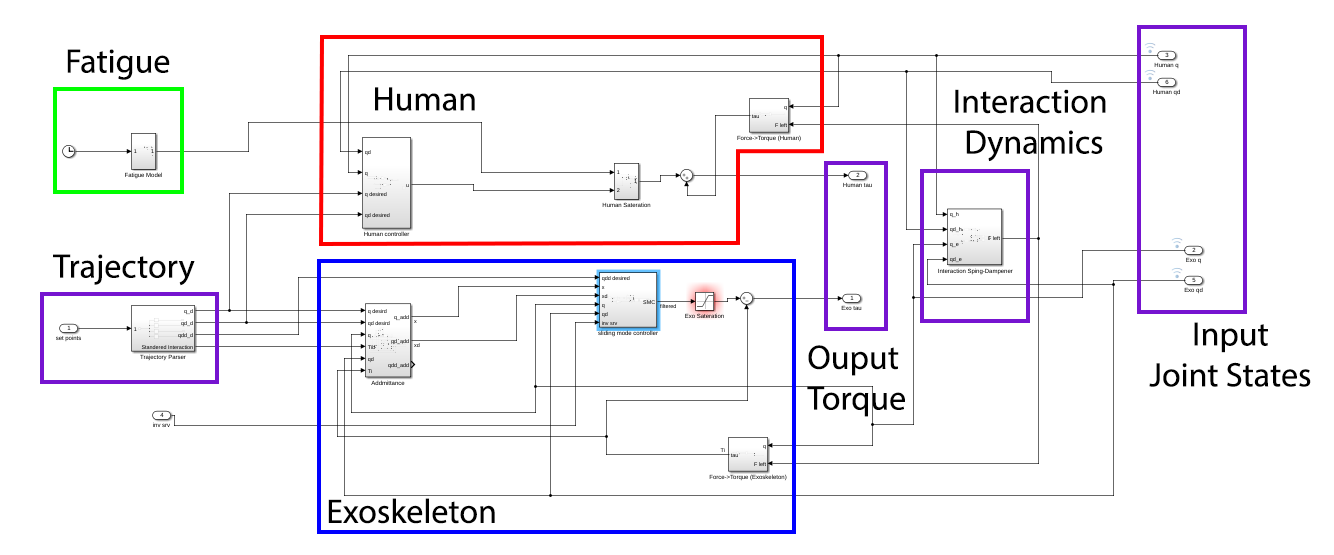
\includegraphics[width=\columnwidth]{images/controllers/upper_model_simulink_edit.png}
    \caption[Simulink Model Cooperative Controller]{Simulink Model of the Cooperative Gait Controller with highlighted subsystems.}
    \label{fig:CoopSimulink}
\end{figure}


\autoref{fig:TripleGaitMotion} shows gait motion with varying human engagement levels. The A-SMC controller compensated for the lack of human involvement and tracked the gait cycle, which is more complex than the previous simple trajectory. The initial start of the controller varies slightly; however, it converges to a steady-state operation and closely tracks the other gait cycles. \autoref{fig:TripleGaitLeg} show how the position of the human leg and the exoskeleton leg differs. There is a slight difference in position, expected since the legs are not rigidly connected but are connected through a spring-dampener system.  




\begin{figure}
    \centering
    \begin{subfigure}{\linewidth}
        \centering
        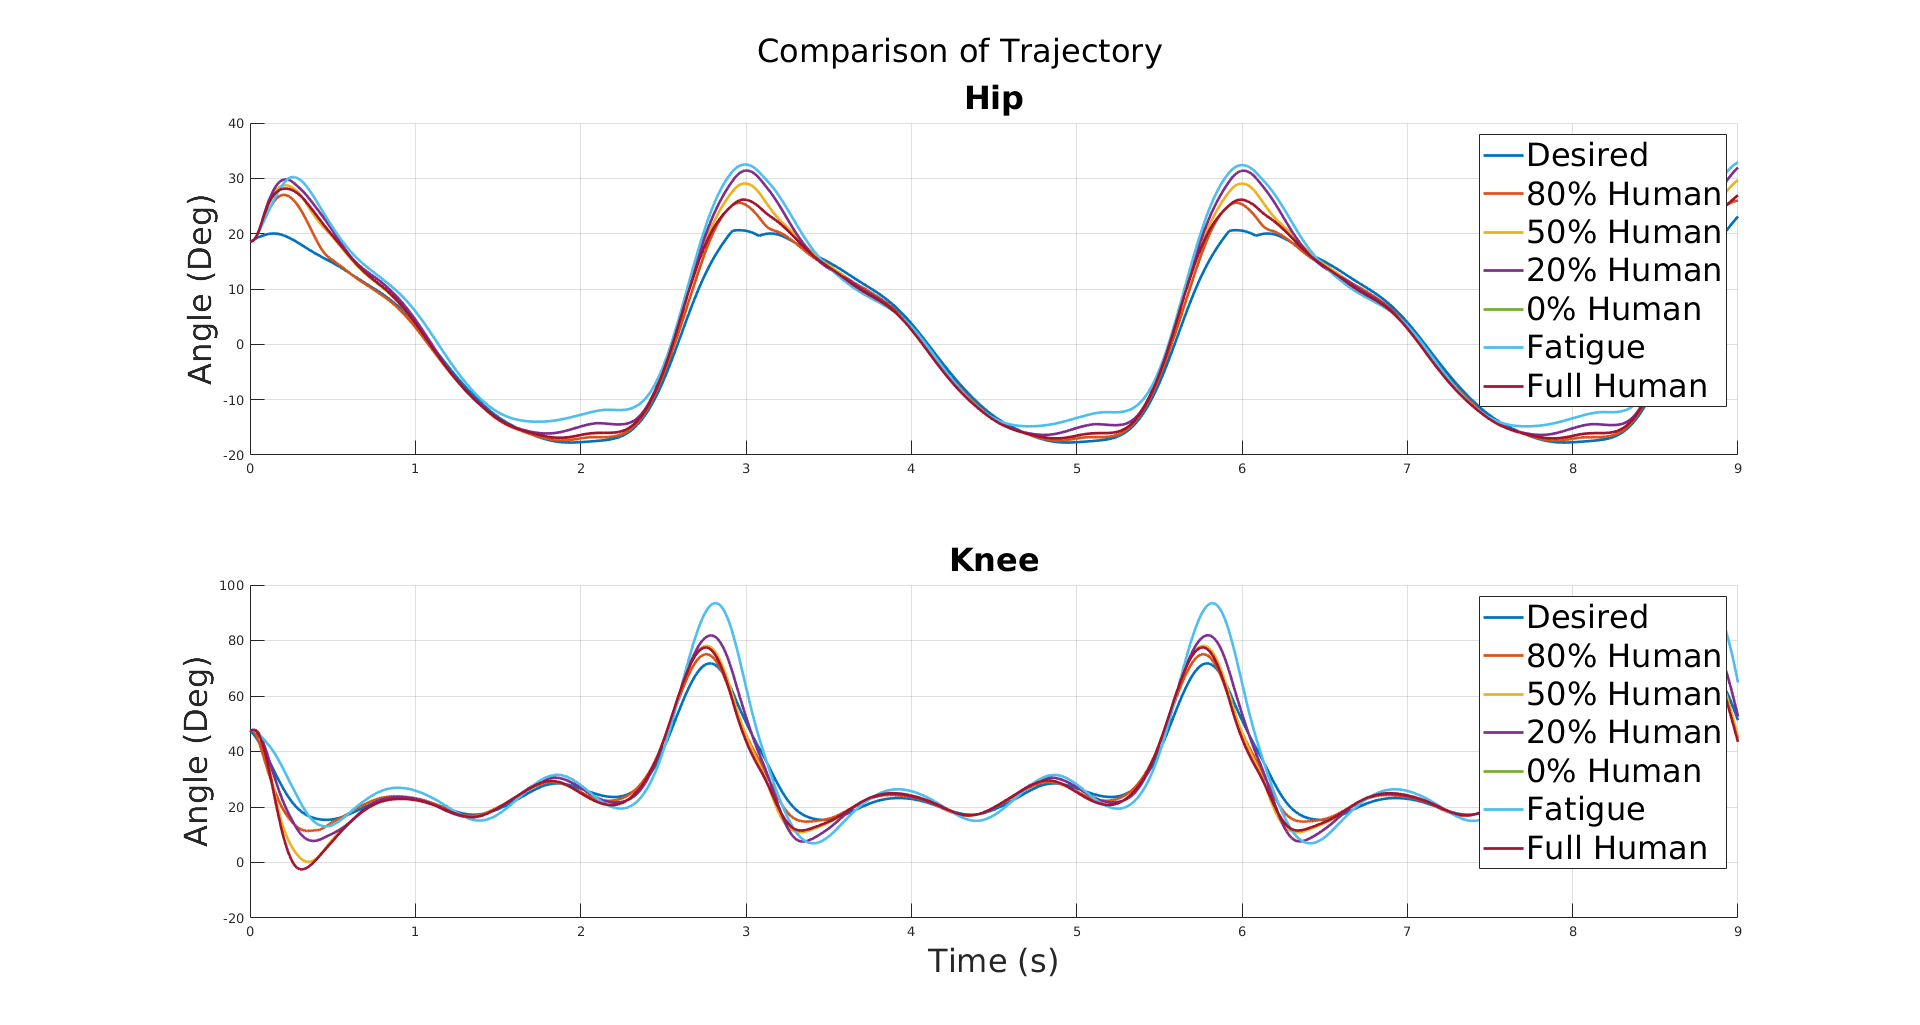
\includegraphics[width=\columnwidth]{images/controllers/gait/traj.png}
        \caption[Comparison of a Triple Gait Cycle]{Comparison of a triple gait cycle at different interaction levels.}
        \label{fig:TripleGaitJoint}
    \end{subfigure}
        \begin{subfigure}{\linewidth}
        \centering
        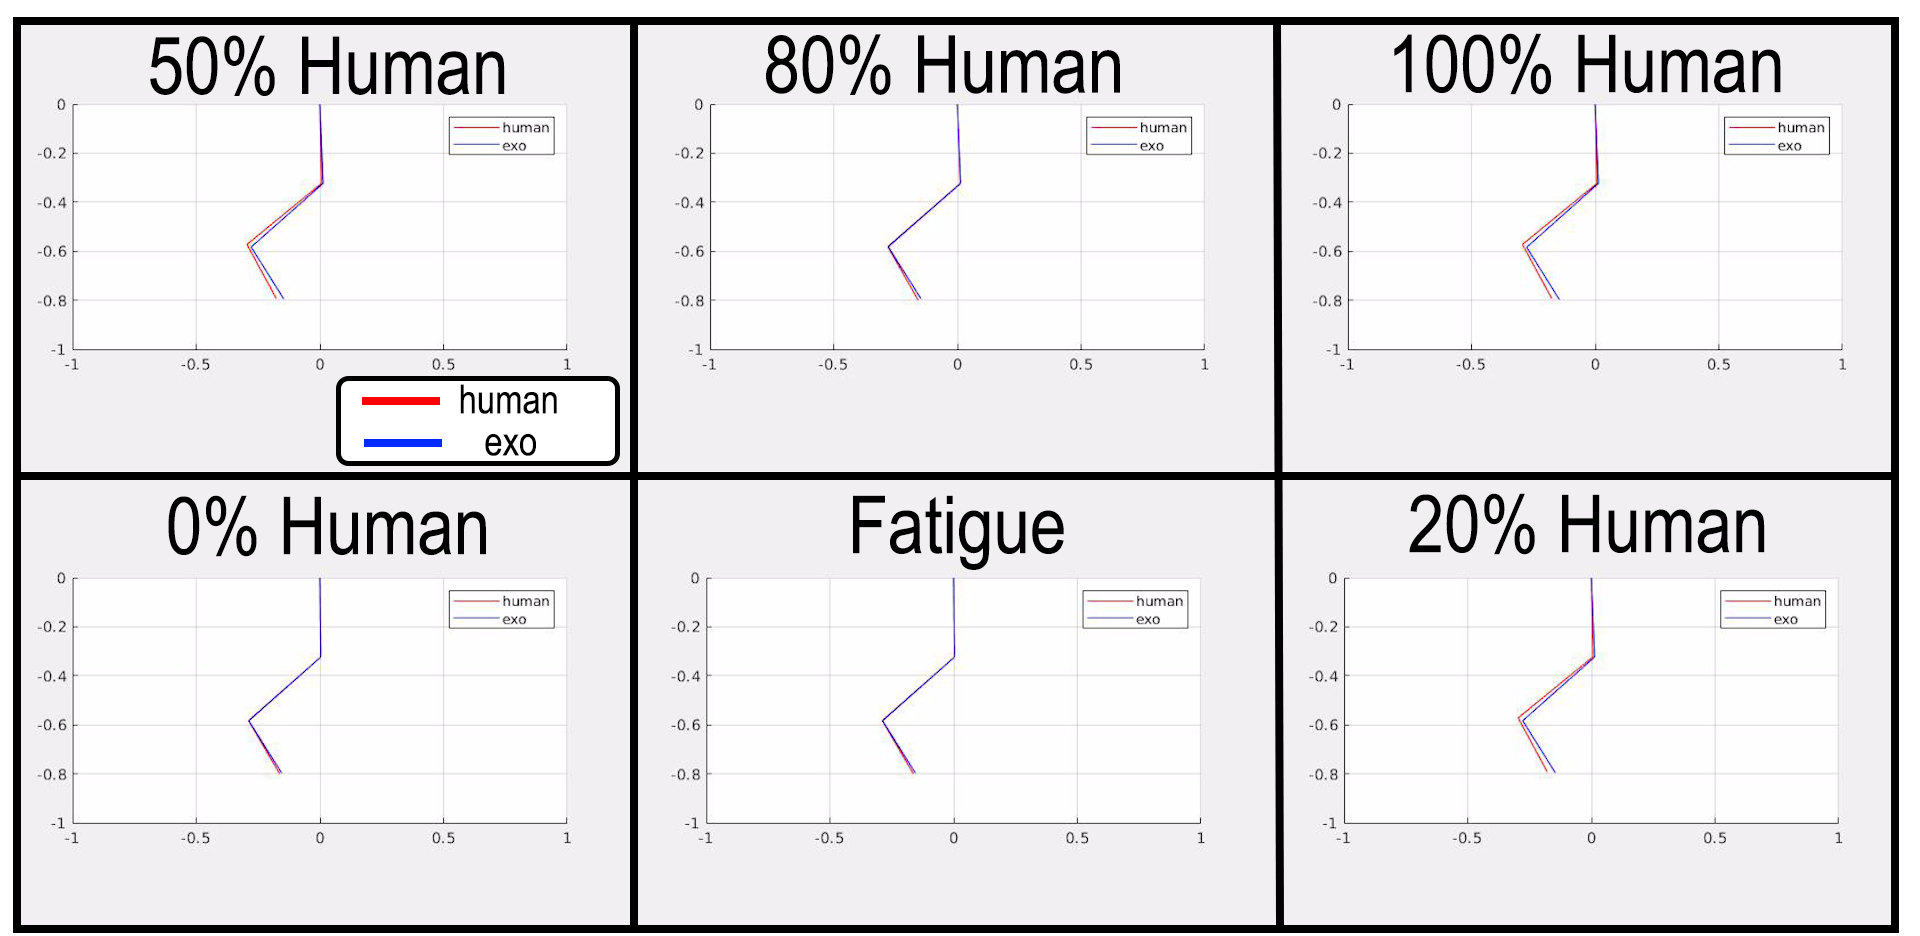
\includegraphics[width=\columnwidth]{images/controllers/gait/leg_frame_annotated.png}
        \caption[Engagement Levels of Leg Motion]{Comparison of the leg motion with the different engagement levels}
        \label{fig:TripleGaitLeg}
    \end{subfigure}
    \caption[Effects of the Different Engagement Levels]{Comparison of the effects of the different engagement levels with a lower limb.}
    \label{fig:TripleGaitMotion}
\end{figure}








\autoref{fig:TorqueOverGaitCycles} shows the torques generated to follow the gait cycles.  \autoref{tab:RMSE} shows the root mean squared error (RSME) of the gait motion. The largest error occurs when there is no human involvement, which is the same as the fatigue involvement. The knee RMSE is slightly larger; this could be due to the knee being the second link that propagates the error down the leg. The RMSE at 100\% error is larger than the error at 80\%; this could be caused since the A-SMC controller handles the interaction as noise, which is larger when there is more human interaction.    

\autoref{fig:HumanTripleGaitMotion} shows the human torques over the gait cycle. The maximum torque is capped at the different levels; this can be seen where the torque does not surpass the maximum activation level. The same fatigue profile shown in \autoref{fig:fatprofile} was used to simulate the muscle fatigue, \autoref{fig:SMCTripleGaitMotion} shows the A-SMC controller torques generated over the gait cycle, and \autoref{fig:InteractionTripleGaitInteration} shows the interaction torques between the human and LARRE. Unlike the simple trajectory model, the human torque profile shown here spikes to the saturation limit. The A-SMC controller torque contains similar profiles observed in the simple trajectory, whereas the human torque decrees, the A-SMC torque increases. Additionally, the controller compensated for the time-varying fatigue, which is critical for operations where the user may not maintain the required torque through the gait cycle. 





\begin{table}
    \centering
    \begin{tabular}{||c || c c c c c c||} 
         \hline
         Joint & 100\% & 80\% & 50\%  & 20\% & 0\% & Fat \\ [0.1ex] 
         \hline\hline
         Hip & 2.7^{\circ} & 2.0^{\circ} & 3.2^{\circ} & 4.1^{\circ} & 5.0^{\circ} & 5.0^{\circ} \\ 
         \hline
         Knee & 4.7^{\circ} & 2.8^{\circ} & 4.4^{\circ}  & 4.2^{\circ} & 7.4^{\circ} & 7.4^{\circ} \\[0.1ex] 
         \hline
    \end{tabular}
    \caption{RMSE (in degrees) of Gait Motion}
    \label{tab:RMSE}
\end{table}

\begin{figure}
    \centering
    \begin{subfigure}{0.8\linewidth}
        \centering
        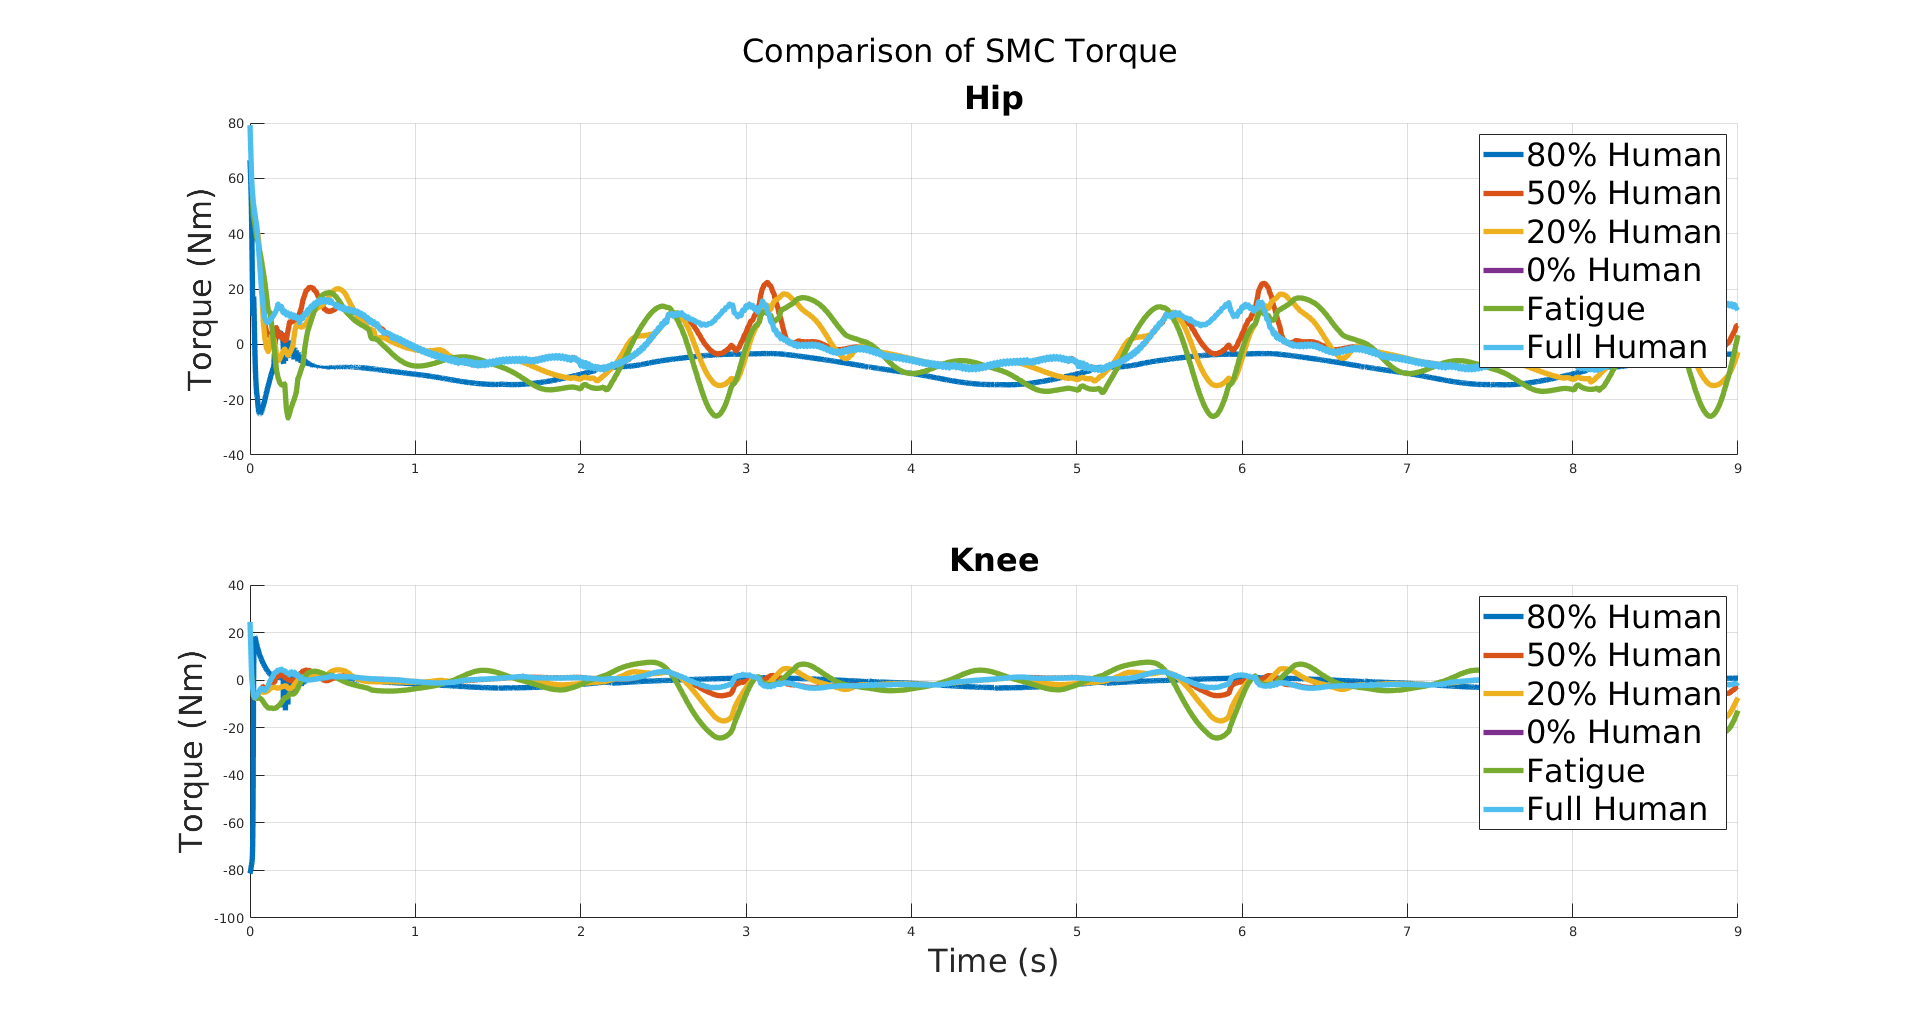
\includegraphics[width=\columnwidth]{images/controllers/gait/SMC.png}
        \caption[A-SMC Torque Over Gait Cycles]{\textit{assistor} (exoskeleton) torque over gait cycles. These torques are generated by the A-SMC controller.}
        \label{fig:SMCTripleGaitMotion}
    \end{subfigure}
    \begin{subfigure}{0.8\linewidth}
        \centering
        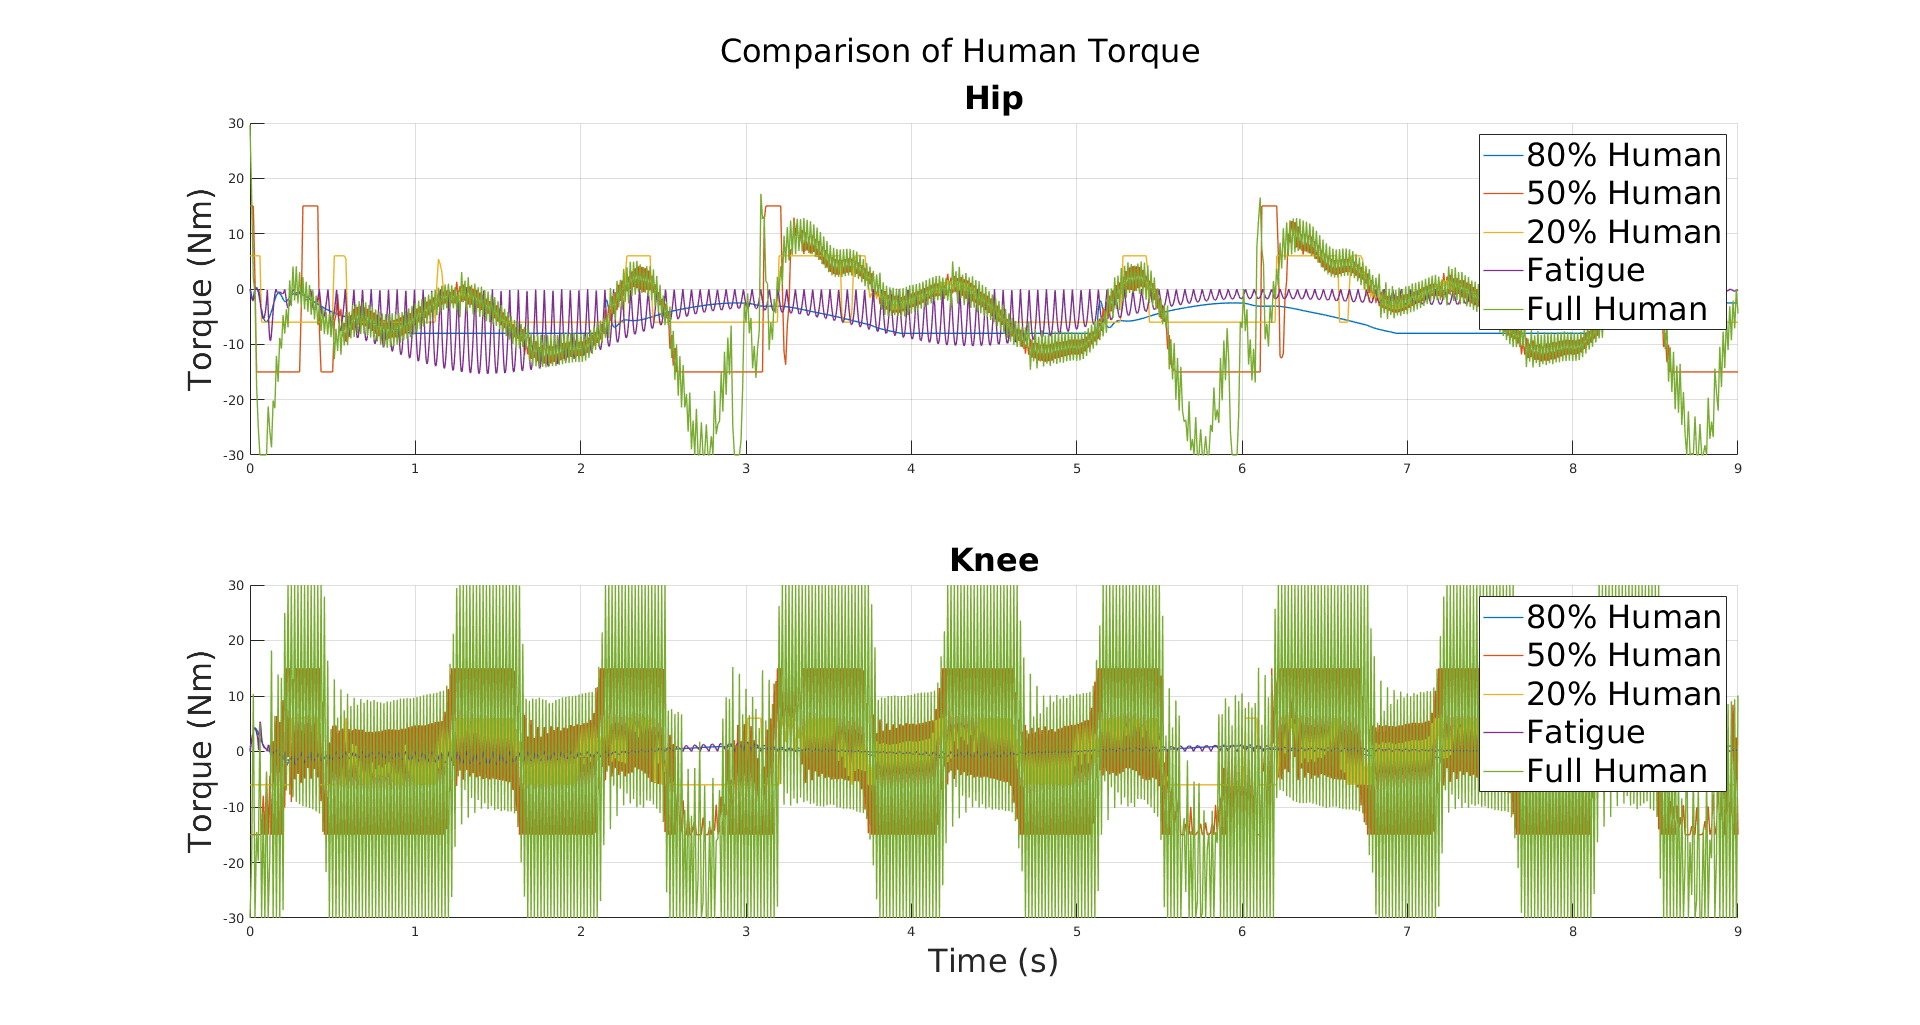
\includegraphics[width=\columnwidth]{images/controllers/gait/human.png}
        \caption[Human Torque Over Gait Cycles]{ \textit{assistie} (Human) torque over gait cycles. These torque are generated by the PD controller.}
        \label{fig:HumanTripleGaitMotion}
    \end{subfigure}
        \begin{subfigure}{0.8\linewidth}
        \centering
        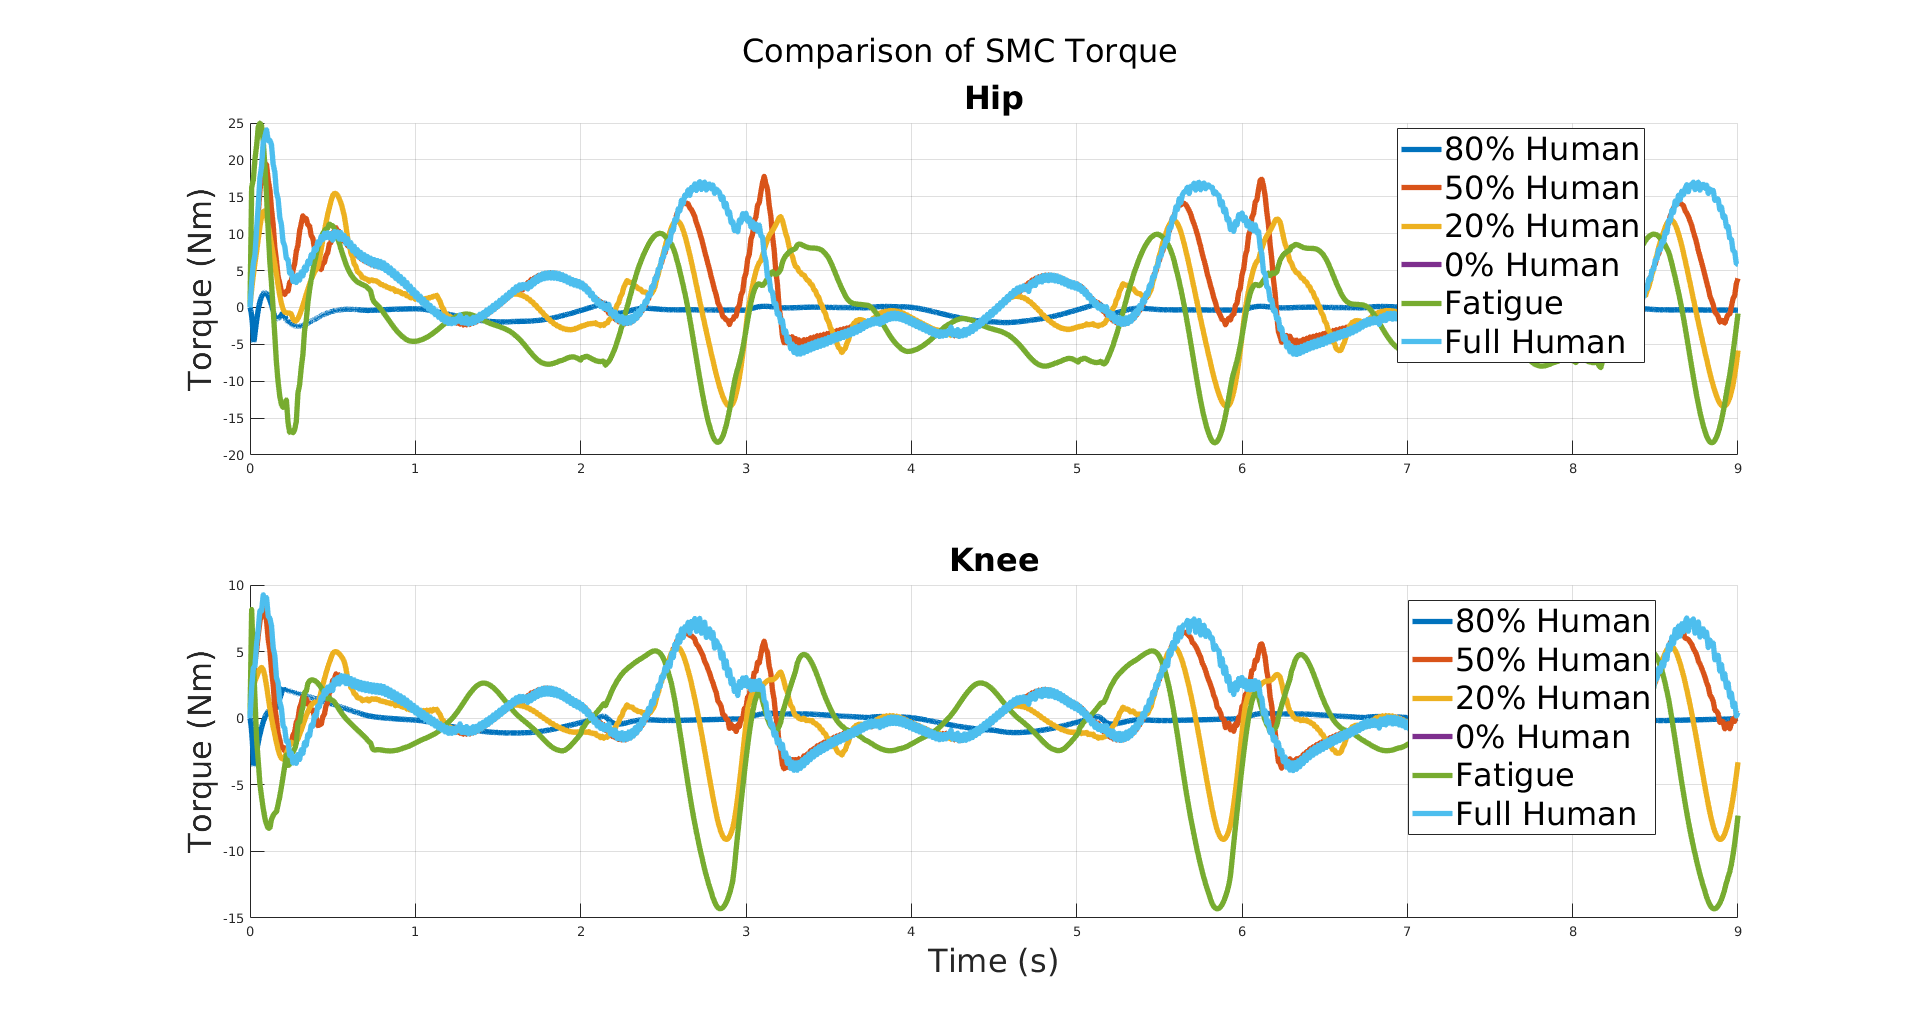
\includegraphics[width=\columnwidth]{images/controllers/gait/feedback.png}
        \caption[Interaction Torque Over Gait Cycles]{Interaction Torque Over Gait Cycles. This is the torque that generated by the displacement between the two systems.}
        \label{fig:InteractionTripleGaitInteration}
    \end{subfigure}
    \caption[Comparison of Torques for Gait Cycle]{Torques generated by the \textit{assistie} (human) and  \textit{assistor} (exoskeleton) controller over three gait cycles. These graphs compare the controller torques generated at the different interactions levels. }
    \label{fig:TorqueOverGaitCycles}
\end{figure}




\subsection{Complication of ROS-Simulink Integration}

The bridge connecting ROS to Simulink seems to be built assuming that a Virtual Machine (VM) runs Linux with the host computer running either Windows or OSX. There are built-in tools to set a connection and use a remote host for ROS; this allows for connection to deploy the node to a robot or allows for development on a non-Linux OS. When a remote host is selected (i.e., not using a localhost), the Simulink node is compiled to the catkin\_ws on the VM. 

A bug in the ROS-Simulink framework was discovered during development. While MATLAB has a process of integrating and using custom messages in Simulink, it has a bug that will only build and compile when the VM is set up to be the ROS master and compile to a VM; this also means that the VM catkin\_ws needs a full copy of all the relevant packages and decencies. This bug was reported to MathWorks\footnote{https://www.mathworks.com/}, who are now fully aware of the bug and are working on a patch for future release. While it is possible to set up such a pipeline, adding a VM into the system significantly complicates the pipeline and adds uncertainly into the controller's timing. 



\section{Validation on Physical System}

The work in this section is still in development. I plan to test the ASMC on the system by having the assistie system act at different engagement levels. The tests will resemble the tests conducted on the simulated system discussed above. I will measure the position and applied torque to both the assistie and assistor systems and compare the measurements to a simulation of the same model.   


To test the controller,  a simple physical system was developed and built; this simplified system shows how the controller works on a real system.  \autoref{eq:armDyn} show the dynamics equation for a single-arm where $m$ is the mass of the arm and $l$ is the length of the arm. This system consists of two single degrees of arms; where one is the \textit{assistie} arm and the other is the \textit{assistor} arm.

\begin{equation}
    \tau = \frac{4}{3}ml^2 \ddot{\theta} + \frac{1}{2}ml \cos(\theta)
    \caption{Dynamics equation of a single arm of the system}
    \label{eq:armDyn}
\end{equation}

 The arms were connected with a Velcro strap piece of foam between the two arms to prevent the arms from bending inward. Each of the arms weighed approximately $90g$ and $0.3m$ long. An additional $20g$ was added to the \textit{assistie} arm to simulate the human system being heavier than the exoskeleton system. \autoref{fig:phyicalTestingSystem} shows the physical testing system. The arms are controlled by brushed DC motors with feedback from potentiometers for position sensing. A computer running Simulink acts as the high-level controller and a Teensy 4.0 \footnote{https://www.pjrc.com/store/teensy40.html} as the low-level controller communicating over a serial line. The motors are controlled by Performance Motion Digital motor controllers (Performance Motion Devices, Inc., 1 Technology Park Dr, Westford, MA 01886). Each of the motors is controlled by a 75W Atlas driver (MD211048/02VB) through the development board (MDK4LI0000V). The Teensy board communicates to the drivers over SPI by sending torque commands to each of the drivers, which delivers the proper current commands to the motors. \autoref{fig:phyicalTestingDiagram} shows the connection diagram; the computer is the high-level controller and the Teensy acts as the low-level controller. 
 
 Application on real hardware comes with several challenges. Real systems must deal with sensor noise and communication speed, affecting how the controller responds to the model updates.  


\begin{figure}
    \centering
    \includegraphics[width=\linewidth]{images/controllers/phyical system.png}
    \caption[Physical A-SMC Testing System]{Physical testing system of two connected arms. A Teensy 4.0 is used as a lower-level controller. Each arm has its own potentiometer and is controlled by a brushed DC motor. The arms are connected by a velcro strap and a piece of foam between the arms prevents the arms from bending inward. The DC motors are controlled by Atlas motor drivers. }
    \label{fig:phyicalTestingSystem}
\end{figure}


\begin{figure}
    \centering
    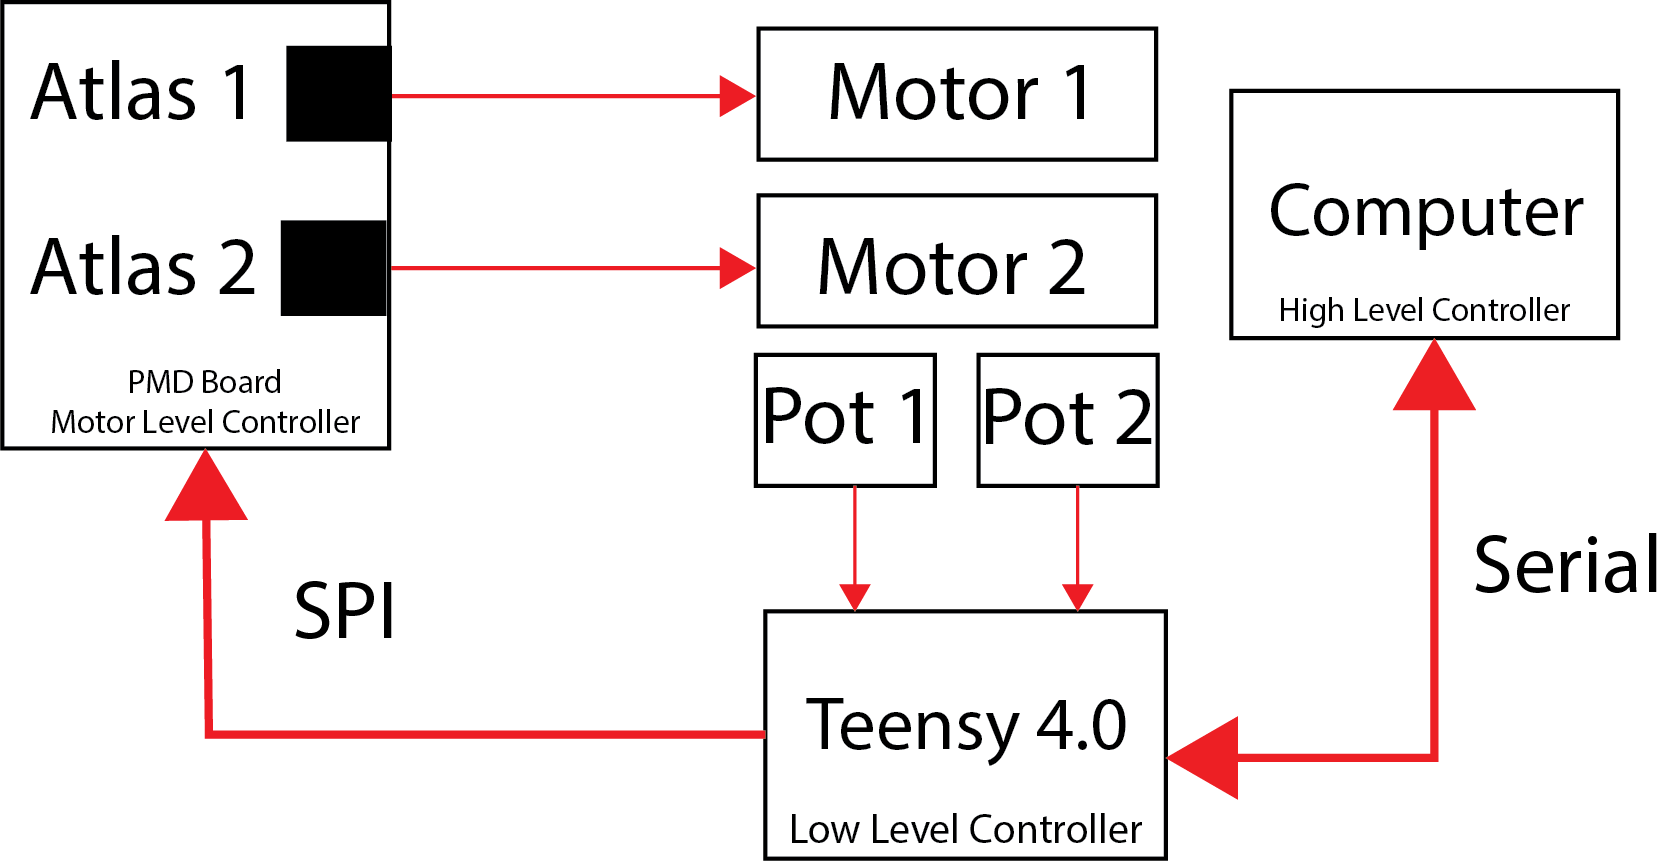
\includegraphics[width=\linewidth]{images/controllers/testing_system_diagam.png}
    \caption[Testing A-SMC System Diagram]{Connection diagram of the testing system. The computer communicates with the Teensy over serial protocol sending shown two torque command and receiving two position. The Teensy uses SPI to communicate with the motor drivers. }
    \label{fig:phyicalTestingDiagram}
\end{figure}



% \subsection{Application of Tuning Methodology}

% The tuning methodology developed for the simplified was applied to tune the cooperative controller for the LARRE. A Simulink model was built with ROS communication to tune the parameters. A model was built to calculate the forward and inverse dynamics on the fly using the \textit{ambf\_control\_system} package. Since this framework uses the same AMBF simulation model, it is a good representation of the dynamics.   



% \subsection{Tuning of LARRE controller}

% The above method was used to tune the controller for LARRE. The model dynamics were calculated using the \textit{ambf\_control\_system} package for both the inverse and forward dynamics, allowing the system's response to be estimated on an identical model to the AMBF model but without the need to run AMBF, which would complicate the learning process. This was accomplished using the built-in ROS-Simulink bridge. 

% The tuning was done on a Ryzen$\texttrademark$ 5900x\footnote{https://www.amd.com/en/products/cpu/amd-ryzen-9-5900x} with $32Gb$ of memory and a Nvidia$\texttrademark$ 2700S GPU\footnote{https://www.nvidia.com/en-us/geforce/graphics-cards/rtx-2070-super/}. Due to many parameters (74 parameters assume that matrix elements off the diagonal are 0), the tuning process had to be done in batches. If too many iterations were attempted, the computer would run out of memory running, causing the computer to crash. To solve this problem, only five iterations were run and restarted the process, with the final parameters of an iteration being the initial parameters of the next run. 




% \autoref{fig:coopCost} Show the converges of the response optimization. For systems with many parameters, upper and lower bound must be defined; this helps bound the search space and reduce optimization time. While the upper bound is hard to determine, the lower bound is known to be greater than 0, the $\beta$ parameter is bound between $0$ and $1$. It is also important to ensure the off-diagonal of the matrix is strictly 0 since only the diagonal elements are required. \autoref{fig:coopParams} shows how the parameters changed over the iterations. Twice the number of iterations is displayed because two resets were allowed in the optimization. They are split into different graphs since the different magnitudes' parameters allow for values to be better displayed. While it is difficult to determine how the parameters affect the overall model, all the parameters are correlated, and the system is highly non-linear. However, we can see that the magnitude of the parameters is critical. While the parameters did vary over time, they did not change magnitude.  


% \begin{figure}[h]
%     \centering
%     \begin{subfigure}{\textwidth}
%         \centering
%         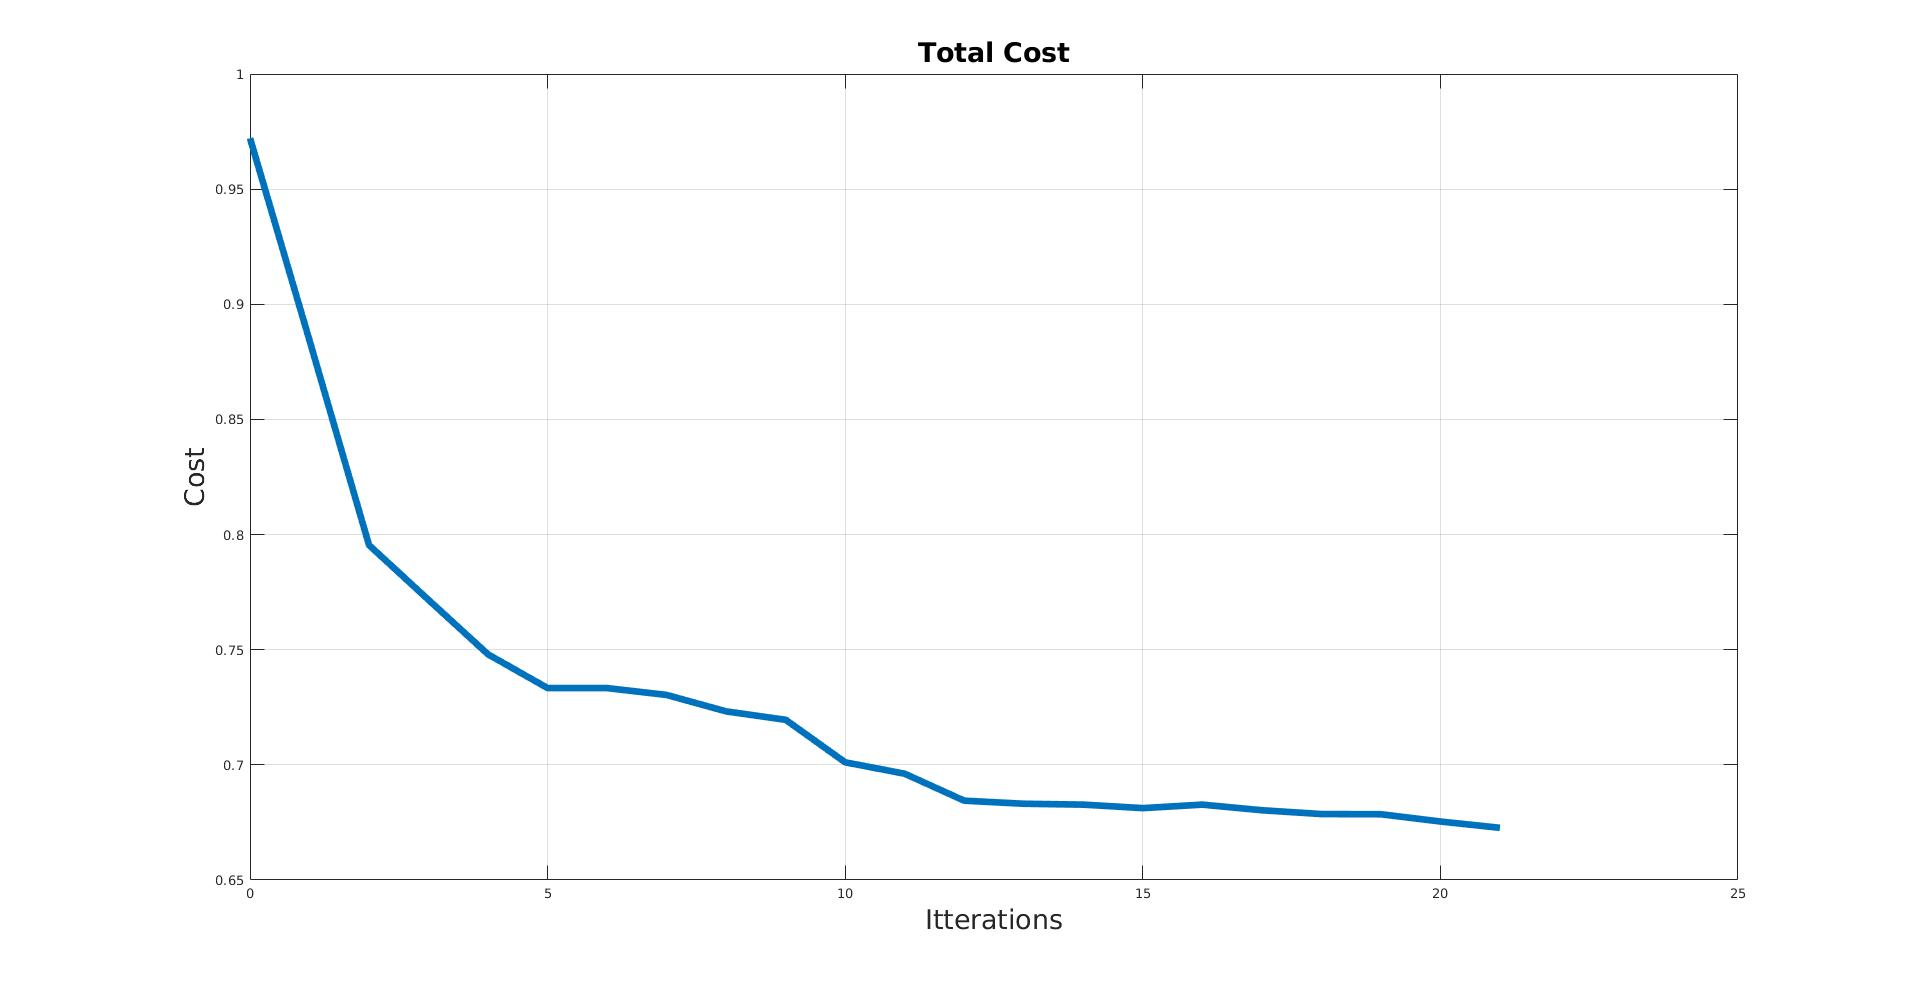
\includegraphics[width=\linewidth]{images/controllers/coop_cost.jpg}
%         \caption[Cost for LARRE Controller]{Cost of tuning the LARRE controller.}
%         \label{fig:coopCost}
%     \end{subfigure}
%     \begin{subfigure}{\textwidth}
%         \centering
%         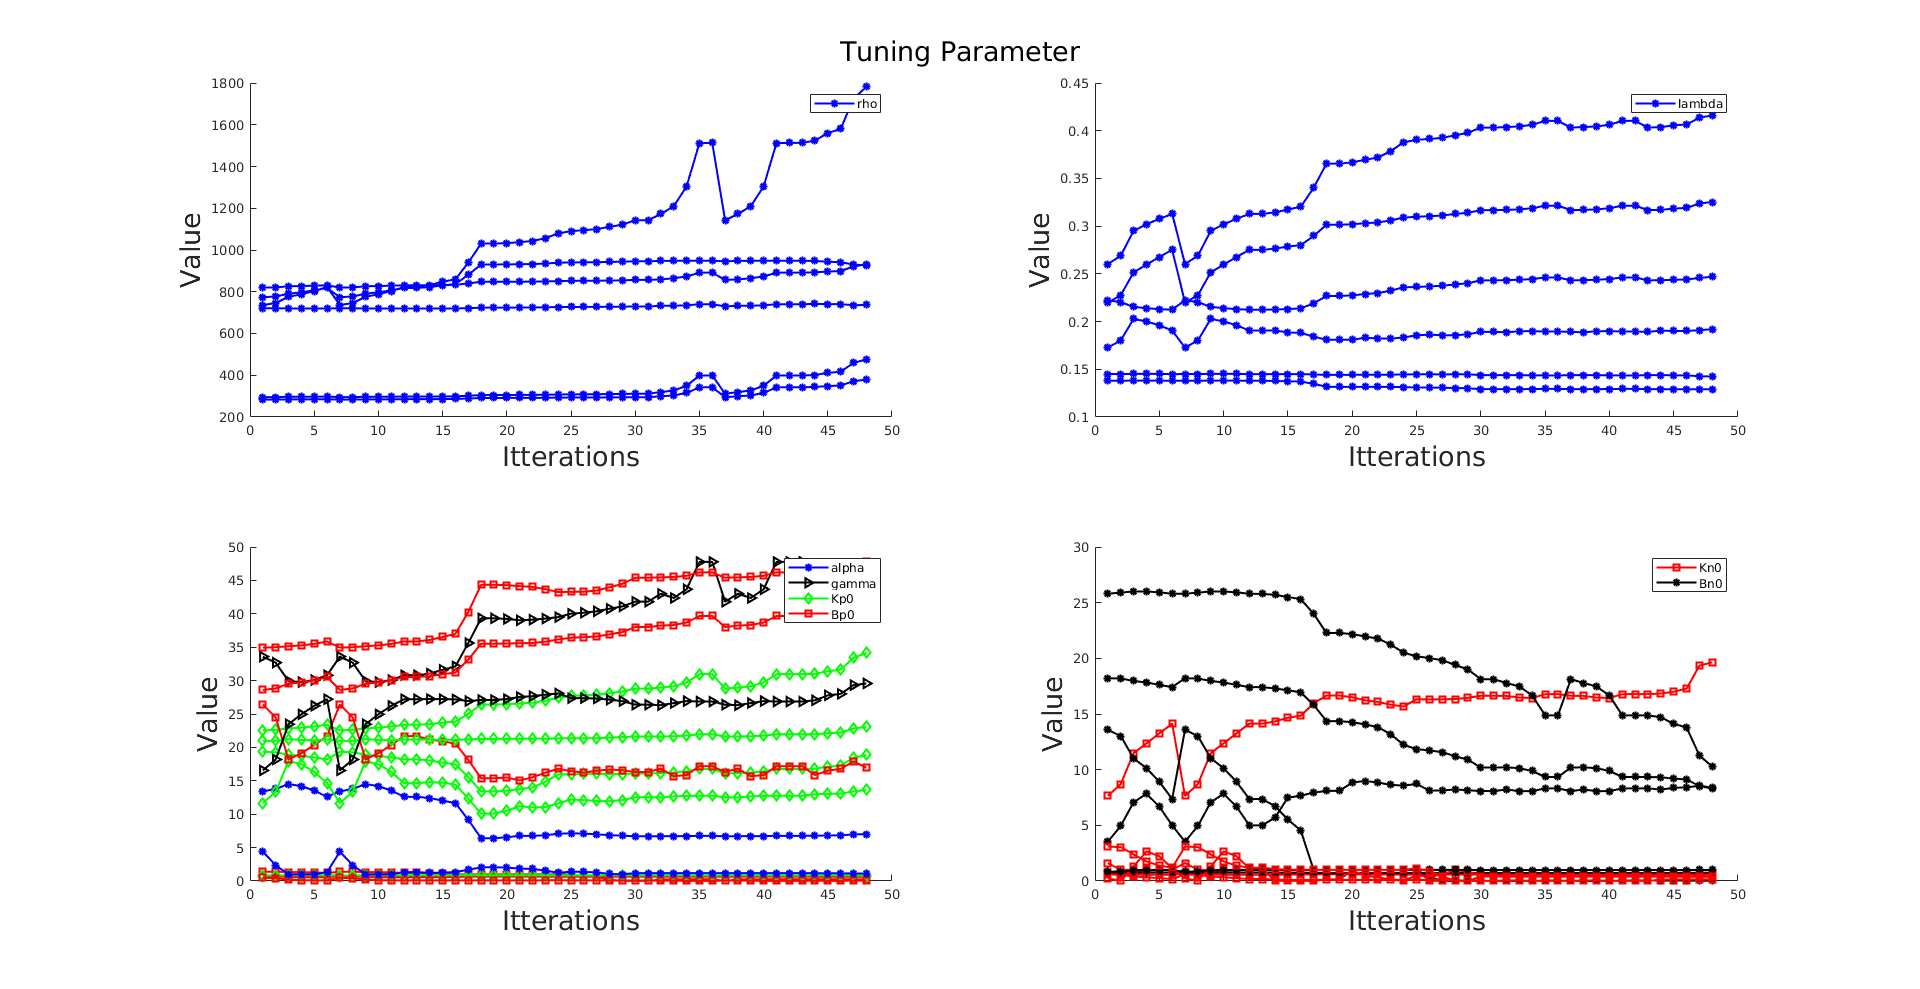
\includegraphics[width=\linewidth]{images/controllers/all_params.png}
%         \caption[Double Pendulum: Positive Alignment-Trajectory]{Trajectories of double pendulum}
%         \label{fig:coopParams}
%     \end{subfigure}
%     \caption[Parameter updates for LARRE Controller]{Parameter updates for LARRE Controller.}
%     \label{fig:coopParams}
% \end{figure}



% \autoref{fig:SMC_connection} shows a high-level overview of the system connections. A virtual machine (VMWare\footnote{https://www.vmware.com/products/workstation-player.html}) was required to run a ROS master due to a bug in the deployment of the Simulink ROS node. The main control system sends set points the Simulink control along with receiving constant state feedback. The Simulink control node calculates the effort and sends it back to the main controller, which sends it down to AMBF. Additionally, the \textit{ambf\_control\_system} is used to calculate the inverse dynamics of the model.   

% \begin{figure}
%     \centering
%     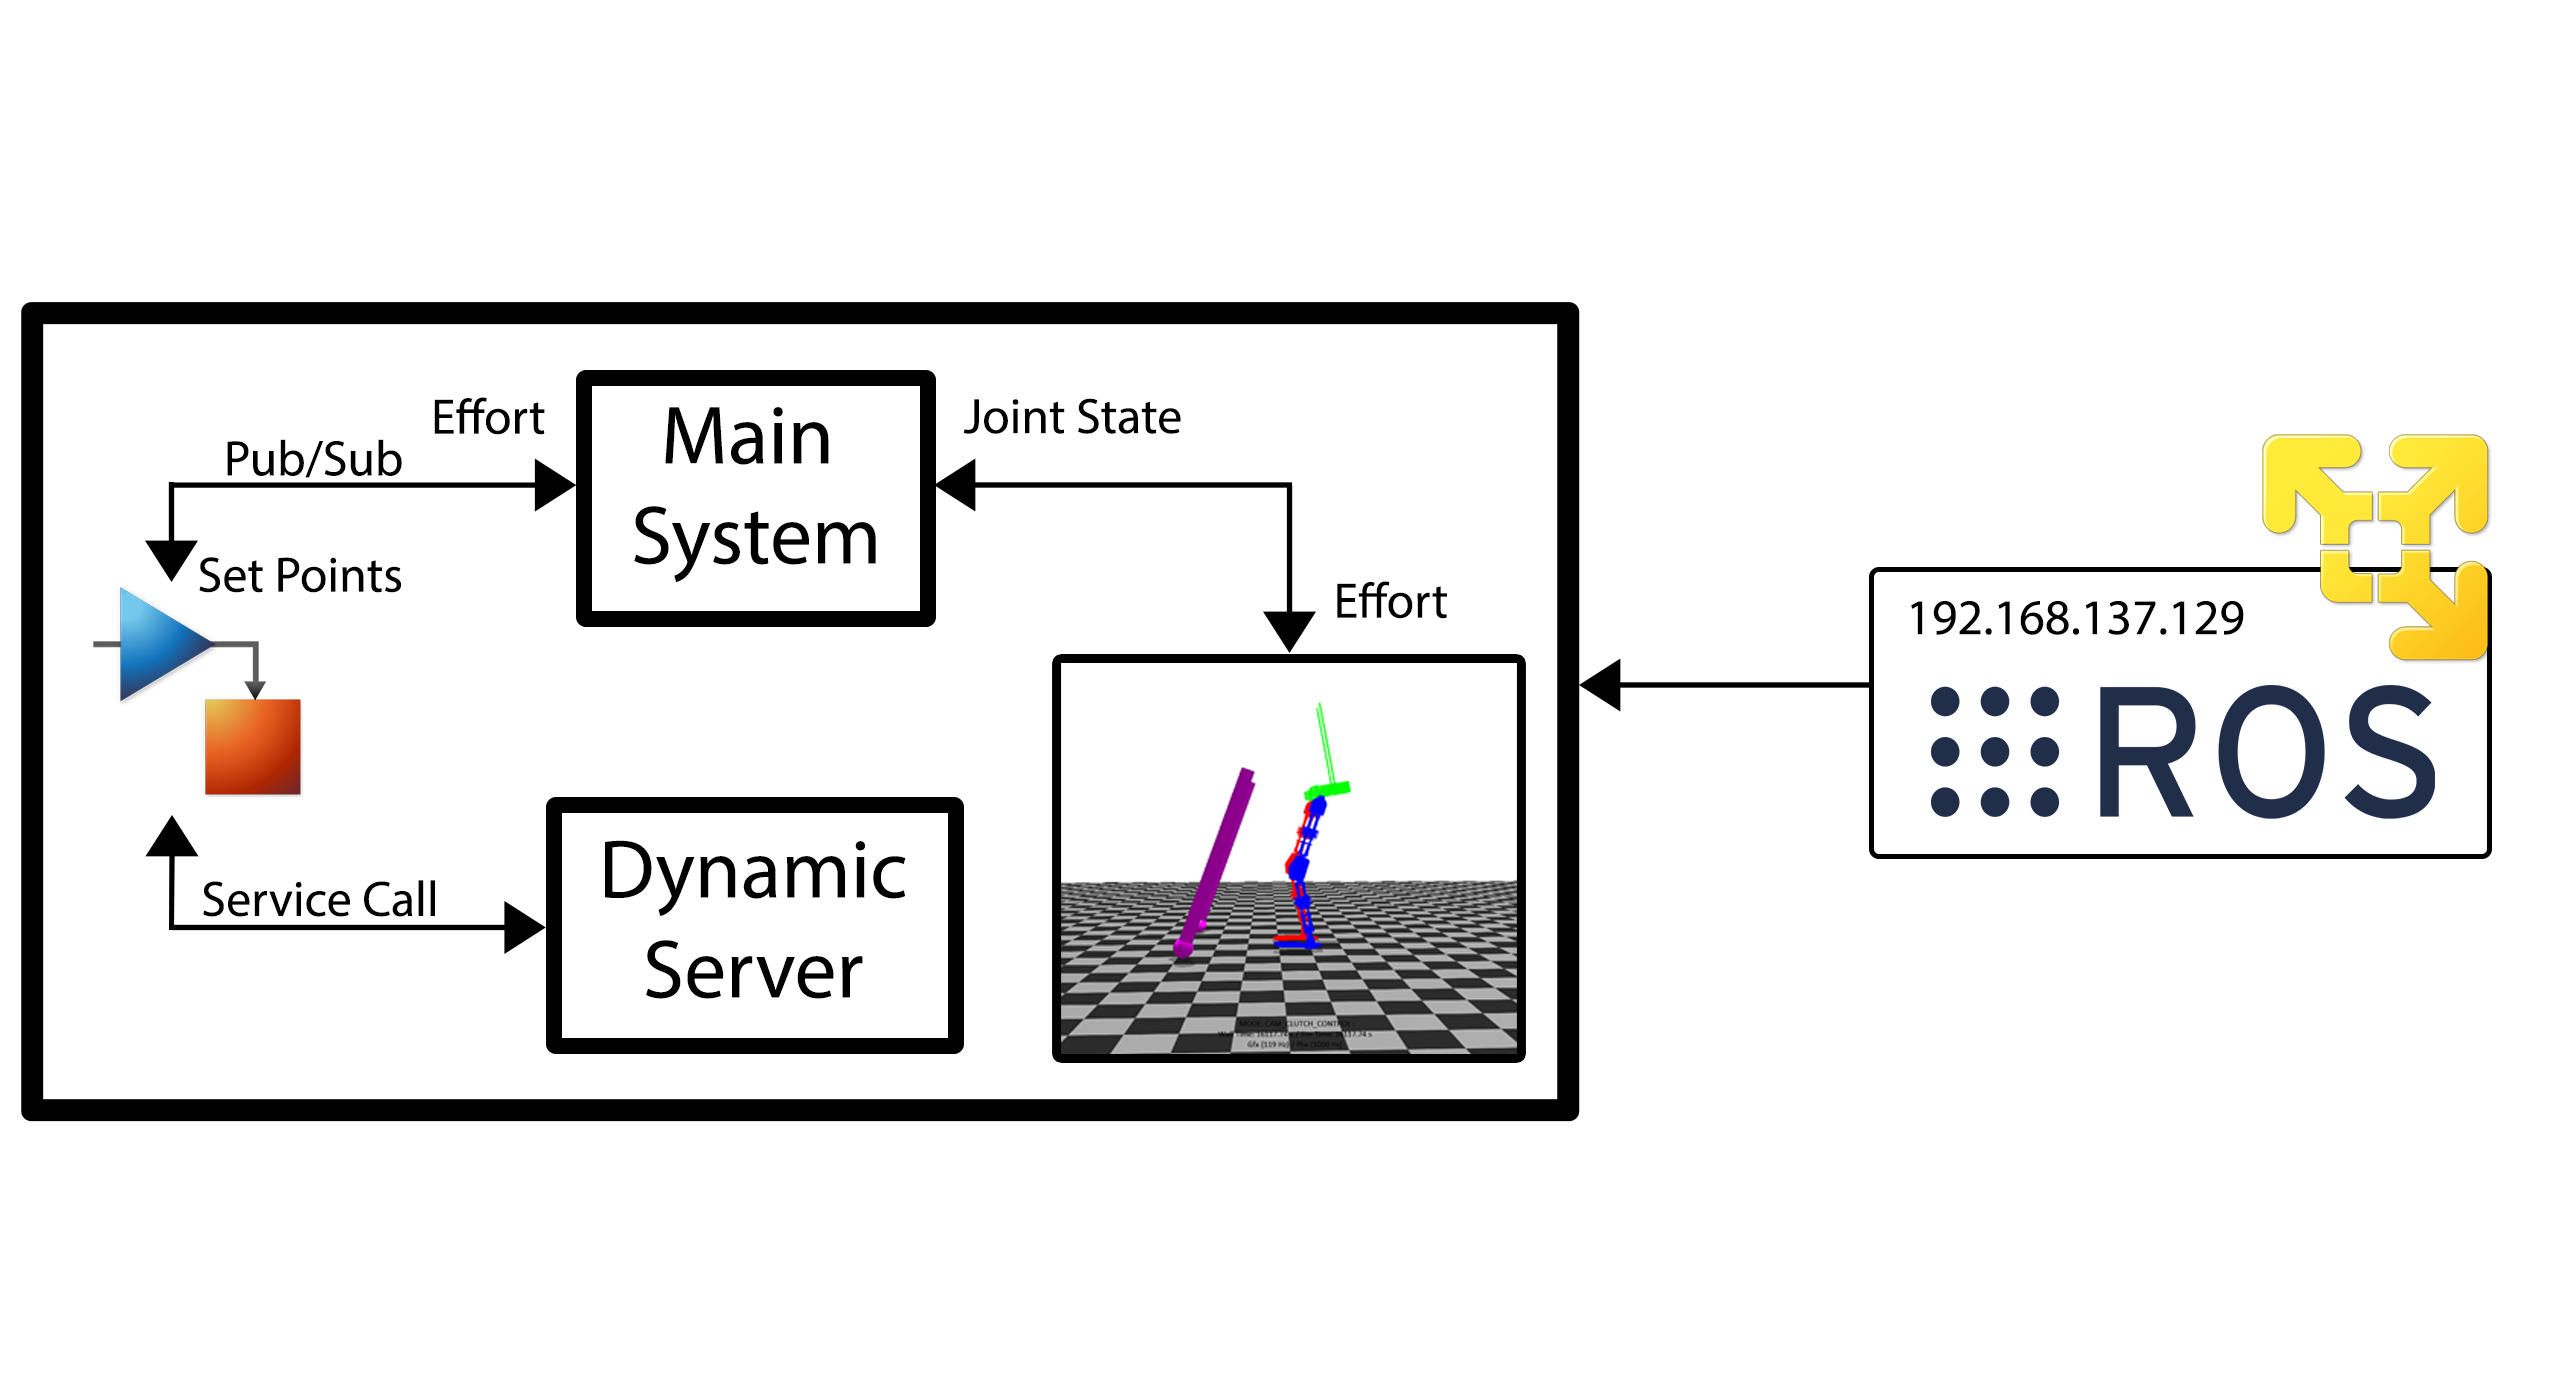
\includegraphics[width=\textwidth]{images/controllers/simulink_connection.png}
%     \caption[SMC Connection Overview]{SMC Connection Overview.}
%     \label{fig:SMC_connection}
% \end{figure}


% The sliding surfaces are shown in \autoref{fig:simple_statespace}. The graphs are shown for the hip, knee, and ankle. The graphs are as smooth as the simple double pendulum model graphs and converge slightly before reaching 0; this can be repeating the optimization method described above until more optimal parameters are calculated; this can also be used to solve the slight bend in all the graphs.  

% \begin{figure}
%     \centering
%     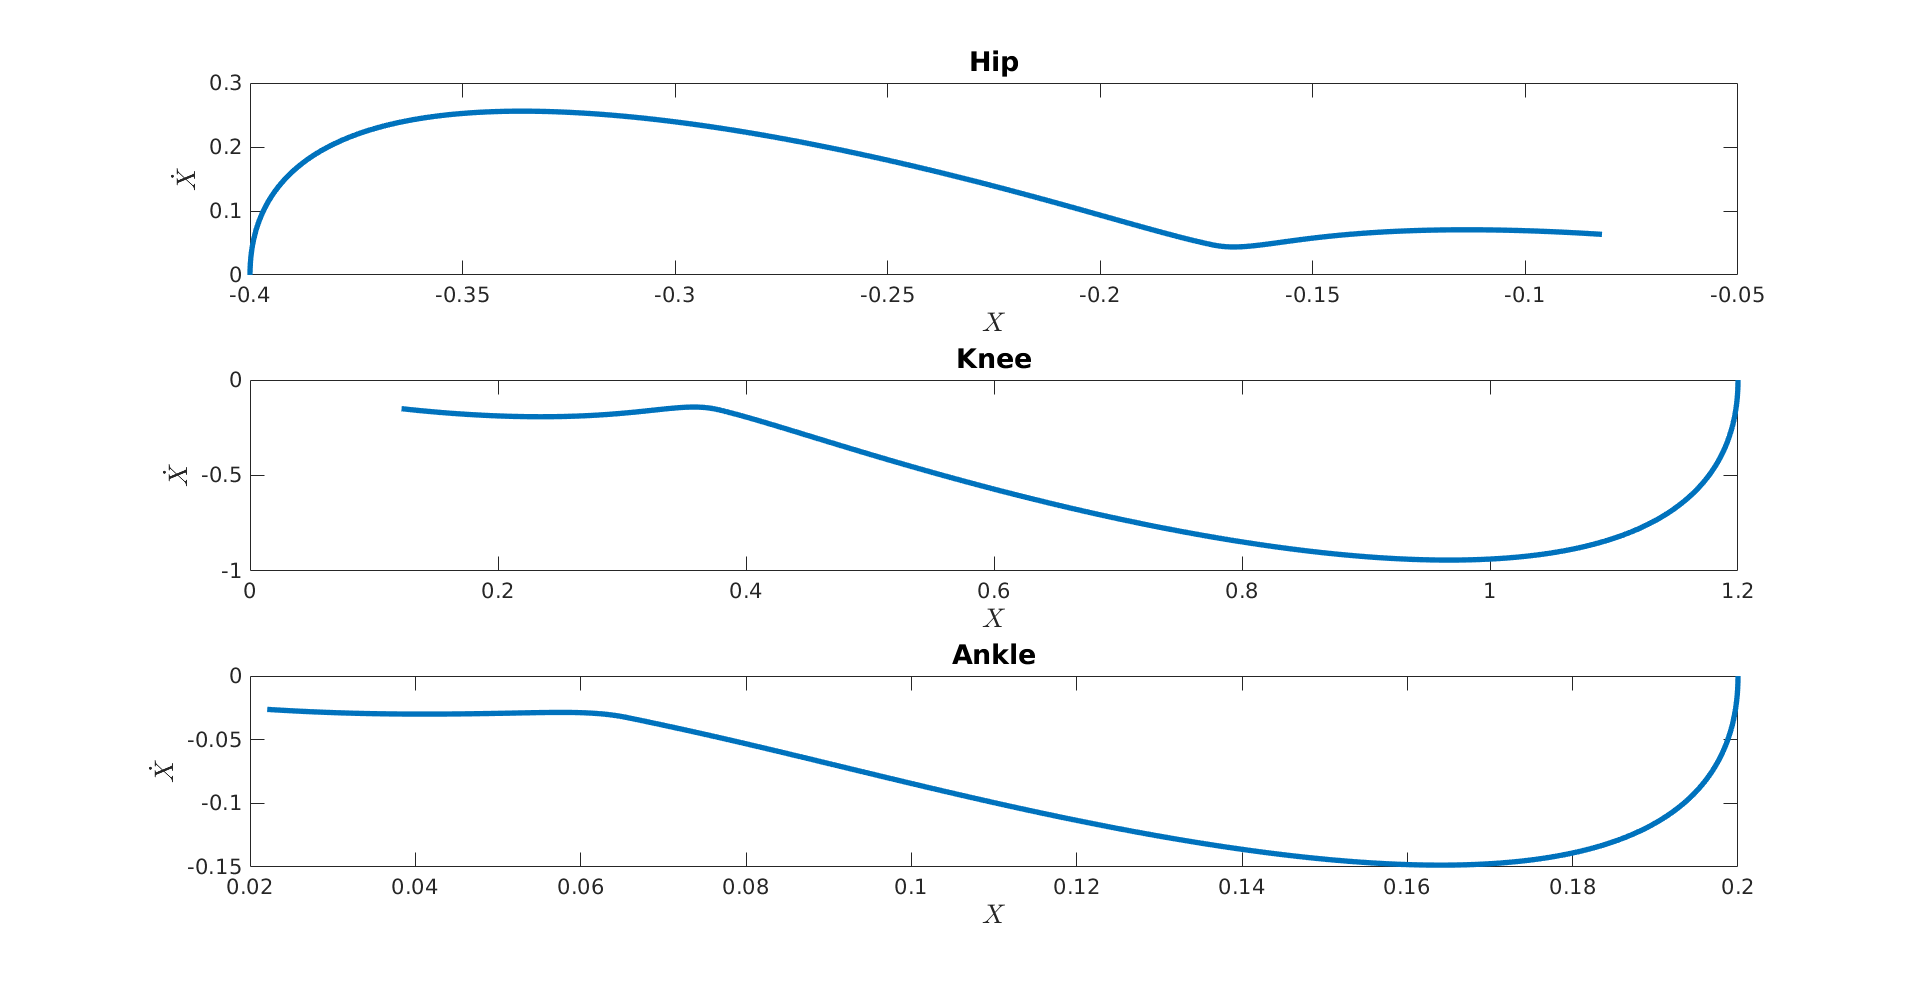
\includegraphics[width=\textwidth]{images/controllers/statespace_simple.png}
%     \caption[Controller State Space]{Controller state space graphs}
%     \label{fig:simple_statespace}
% \end{figure}


% \subsection{Complication of ROS-Simulink Integration}

% The bridge connecting ROS to Simulink seems to be built assuming that a virtual machine (VM) runs Linux with the host computer running either Windows or OSX. There are built-in tools to set a connection and use a remote host for ROS; this allows for connection to deploy the node to a robot or allows for development on a non-Linux OS. When are remote host is selected (i.e., not using a localhost), the Simulink node is compiled to the catkin\_ws on the VM. 

% A bug in the ROS-Simulink framework was discovered during development. While MATLAB has a process of integrating and using custom messages in Simulink, it has a bug that will only build and compile when you set up a VM to be the ROS master and compile to that VM. It does work when you use the \textit{Play} method; however, this is an order of magnitude slower as shown in \autoref{fig:SimulinkTimingComparison}. Building and compiling the controller into a ROS node has a lower mean and variance than playing the model; this is important since if the controller runs too slowly and the timing is inconsistent, the controller will not perform properly; this also means that the VM catkin\_ws needs a full copy of all the relevant packages and decencies. This bug was reported to MathWorks\footnote{https://www.mathworks.com/}, who are now fully aware of the bug and are working on a patch for a future release. 


% \begin{figure}
%     \centering
%     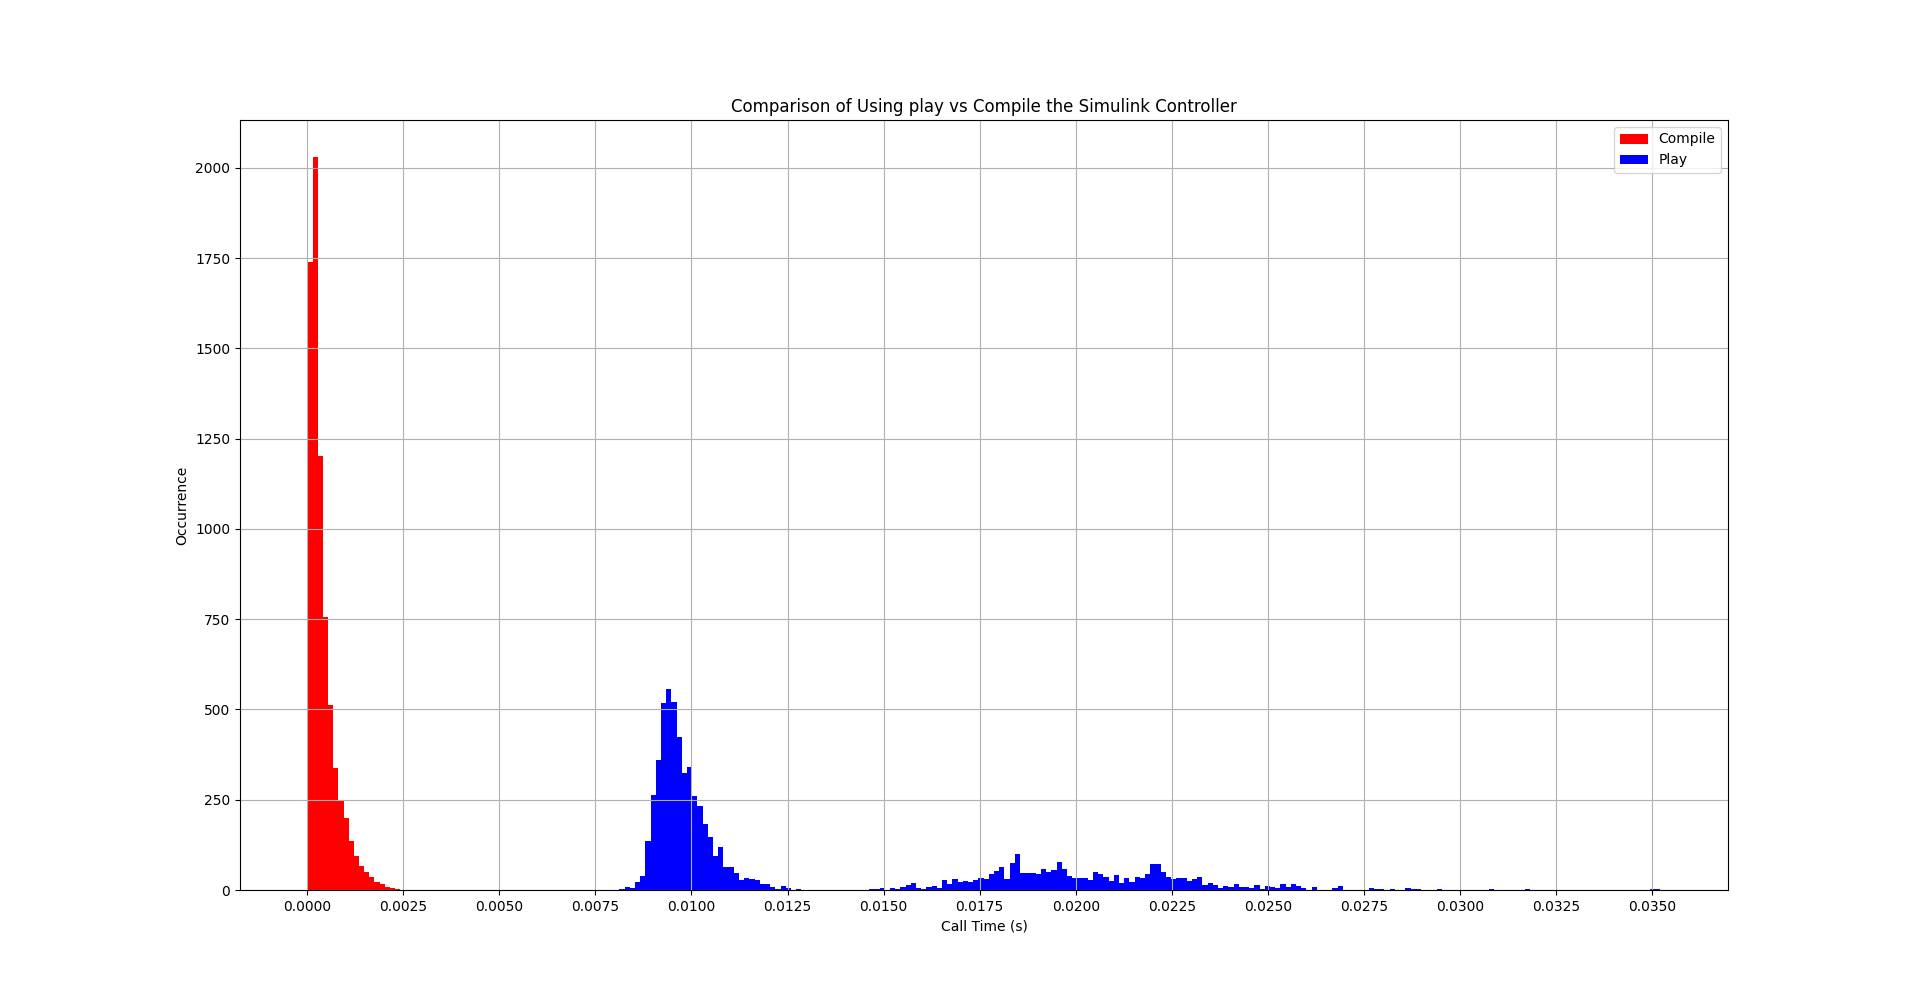
\includegraphics[scale=0.35]{images/controllers/timing_comparison.png}
%     \caption[Simulink Timing Comparison]{Timing Comparison of using the \textit{Build and Run} vs \textit{Play} method}
%     \label{fig:SimulinkTimingComparison}
% \end{figure}

% Additionally, another problem was with the ROS-Simulink communication, which caused the MATLAB to lose track of message definitions and enter an inescapable loop that seized the OS's focus and corrupted the matlabpref file. This problem could only be solved by hard rebooting the computer. Once the computer was rebooted, the \textit{matlabpref} had to be deleted, and all the custom ROS message files had to be re-linked. The cause of this bug is still unknown.





